\documentclass[11pt,]{article}
\usepackage[left=1in,top=1in,right=1in,bottom=1in]{geometry}
\newcommand*{\authorfont}{\fontfamily{phv}\selectfont}
\usepackage[]{mathpazo}


  \usepackage[T1]{fontenc}
  \usepackage[utf8]{inputenc}



\usepackage{abstract}
\renewcommand{\abstractname}{}    % clear the title
\renewcommand{\absnamepos}{empty} % originally center

\renewenvironment{abstract}
 {{%
    \setlength{\leftmargin}{0mm}
    \setlength{\rightmargin}{\leftmargin}%
  }%
  \relax}
 {\endlist}

\makeatletter
\def\@maketitle{%
  \newpage
%  \null
%  \vskip 2em%
%  \begin{center}%
  \let \footnote \thanks
    {\fontsize{18}{20}\selectfont\raggedright  \setlength{\parindent}{0pt} \@title \par}%
}
%\fi
\makeatother




\setcounter{secnumdepth}{3}

\usepackage{longtable,booktabs}

\usepackage{graphicx,grffile}
\makeatletter
\def\maxwidth{\ifdim\Gin@nat@width>\linewidth\linewidth\else\Gin@nat@width\fi}
\def\maxheight{\ifdim\Gin@nat@height>\textheight\textheight\else\Gin@nat@height\fi}
\makeatother
% Scale images if necessary, so that they will not overflow the page
% margins by default, and it is still possible to overwrite the defaults
% using explicit options in \includegraphics[width, height, ...]{}
\setkeys{Gin}{width=\maxwidth,height=\maxheight,keepaspectratio}

\title{Asociación y composición florística de la familia Sapotaceae en la
parcela permanente de 50h, Isla Barro Colorado  }



\author{\Large Merali Rosario\vspace{0.05in} \newline\normalsize\emph{Estudiante, Universidad Autónoma de Santo Domingo (UASD)}  }


\date{}

\usepackage{titlesec}

\titleformat*{\section}{\normalsize\bfseries}
\titleformat*{\subsection}{\normalsize\itshape}
\titleformat*{\subsubsection}{\normalsize\itshape}
\titleformat*{\paragraph}{\normalsize\itshape}
\titleformat*{\subparagraph}{\normalsize\itshape}

\titlespacing{\section}
{0pt}{36pt}{0pt}
\titlespacing{\subsection}
{0pt}{36pt}{0pt}
\titlespacing{\subsubsection}
{0pt}{36pt}{0pt}





\newtheorem{hypothesis}{Hypothesis}
\usepackage{setspace}

\makeatletter
\@ifpackageloaded{hyperref}{}{%
\ifxetex
  \PassOptionsToPackage{hyphens}{url}\usepackage[setpagesize=false, % page size defined by xetex
              unicode=false, % unicode breaks when used with xetex
              xetex]{hyperref}
\else
  \PassOptionsToPackage{hyphens}{url}\usepackage[unicode=true]{hyperref}
\fi
}

\@ifpackageloaded{color}{
    \PassOptionsToPackage{usenames,dvipsnames}{color}
}{%
    \usepackage[usenames,dvipsnames]{color}
}
\makeatother
\hypersetup{breaklinks=true,
            bookmarks=true,
            pdfauthor={Merali Rosario (Estudiante, Universidad Autónoma de Santo Domingo (UASD))},
             pdfkeywords = {Diversidad, Sapotaceae, Riqueza, Abundancia, Asociación},  
            pdftitle={Asociación y composición florística de la familia Sapotaceae en la
parcela permanente de 50h, Isla Barro Colorado},
            colorlinks=true,
            citecolor=blue,
            urlcolor=blue,
            linkcolor=magenta,
            pdfborder={0 0 0}}
\urlstyle{same}  % don't use monospace font for urls

% set default figure placement to htbp
\makeatletter
\def\fps@figure{htbp}
\makeatother

\usepackage{pdflscape} \newcommand{\blandscape}{\begin{landscape}}
\newcommand{\elandscape}{\end{landscape}} \usepackage{float}
\floatplacement{figure}{H}
\newcommand{\beginsupplement}{ \setcounter{table}{0} \renewcommand{\thetable}{S\arabic{table}} \setcounter{figure}{0} \renewcommand{\thefigure}{S\arabic{figure}} }


% add tightlist ----------
\providecommand{\tightlist}{%
\setlength{\itemsep}{0pt}\setlength{\parskip}{0pt}}

\begin{document}
	
% \pagenumbering{arabic}% resets `page` counter to 1 
%
% \maketitle

{% \usefont{T1}{pnc}{m}{n}
\setlength{\parindent}{0pt}
\thispagestyle{plain}
{\fontsize{18}{20}\selectfont\raggedright 
\maketitle  % title \par  

}

{
   \vskip 13.5pt\relax \normalsize\fontsize{11}{12} 
\textbf{\authorfont Merali Rosario} \hskip 15pt \emph{\small Estudiante, Universidad Autónoma de Santo Domingo (UASD)}   

}

}








\begin{abstract}

    \hbox{\vrule height .2pt width 39.14pc}

    \vskip 8.5pt % \small 

\noindent La diversidad y estructura de los bosques miden los recursos y la
abundancia en un área geográfica, por ejemplo, los bosques de la familia
Sapotaceae son importantes para proporcionar alimentos a las especies de
vida silvestre. La Isla Barro Colorado es una reserva natural ubicada en
el lago Gatún del Canal de Panamá. Debido a su capacidad de
investigación, es una de las regiones tropicales más conocidas en
materia de biología y ecología tropical. La distribución actual de la
abundancia de especies en BCI se atribuye principalmente a los
mecanismos que definen comunidades específicas, como la prevalencia de
especies dominantes. Sin embargo, la distribución de la abundancia
relativa se ve afectada por interacciones que aún no se han determinado
plenamente, ni en qué grado inciden en la estructura de la comunidad. El
objetivo de este trabajo es determinar la asociación, composición
florística y distribución de la familia Sapotaceae en la parcela
permanente de 50h de la isla Barro Colorado. Los datos de cada uno de
los cuadrantes de una hectárea que componen BCI fueron procesados en R,
teniendo en cuenta la matriz ambiental y la matriz de comunidad, los
cuales contienen datos de las variables ambientales, tales como
condiciones edáficas, tipo de hábitat, topografía del lugar,
clasificación etaria del bosque, datos demográficos y geoferenciación
espacial de todos los individuos censados. Se adaptaron scripts
reproducibles, utilizando colecciones de paquetes multifuncionales.
Todos los datos fueron examinados utilizando análisis de ecología
númerica. Se registraron un total de 5 especies y 2 géneros distribuidos
en 2029 individuos en toda la parcela. La riqueza por cuadro fue de 4
especies y la mediana de la abundancia por cuadro fue de 39 individuos.
La especie más abundante fue \emph{Pouteria reticulata}, con 1084
individuos, y la menos abundante fue \emph{Pouteria fossicola} con 3
individuos. La riqueza de la familia Sapotaceae presenta correlación con
la presencia de cobre y nitrógeno en el suelo. Las variables
geomorfológicas presentan asociación con la abundancia y riqueza. La
riqueza de la familia Sapotaceae aumenta en función del contenido de
hidrógeno, nitrógeno y cobre, Ademas, aunmenta con la equidad. Los
índices de diversidad alfa arrojaron valores muy bajos. Las especies que
contribuyen de manera significativa a la diversidad beta fueron:
\emph{Chrysophyllum argenteum} , \emph{Chrysophyllum cainito} y
\emph{Pouteria stipitata}, de las cuales la que mas contribuyó a la
diversidad beta fué \emph{Chrysophyllum cainito}. De acuerdo con estos
resultados, se concluye que la riqueza de la familia Sapotaceea no
presenta mucha diversidad en BCI, lo cual se estima que la riqueza
seguiría constante o no aumentaría significativamente aunque se hiciera
un mayor esfuerzo de muestreo


\vskip 8.5pt \noindent \emph{Keywords}: Diversidad, Sapotaceae, Riqueza, Abundancia, Asociación \par

    \hbox{\vrule height .2pt width 39.14pc}



\end{abstract}


\vskip 6.5pt


\noindent  \section{Introducción}\label{introducciuxf3n}

La diversidad y estructura de los bosques miden los recursos y la
abundancia en un área geográfica, y cumplen funciones elementales para
mantener la vida, por ejemplo, los bosques tropicales poseen una gran
diversidad de especies y complejidad ecológica. Además, cubren un 10\%
de la superficie terrestre y son de gran importancia para el planeta,
debido a que capturan y procesan inmensas cantidades de carbono
(Campos-Pineda, Moreno, \& Mendieta, 2017; Martínez-Sovero et al.,
2021).

La familia Sapotaceae está ampliamente distribuida en las zonas
tropicales (Smedmark, 2007). Producen frutas tropicales y algunas
especies producen látex, y madera de alta calidad, siendo una familia de
plantas de importancia ecológica y económica (Martínez-Sovero,
Iglesias-Osores, \& Villena-Velásquez, 2020). Los bosques de la familia
Sapotaceae son importantes para proporcionar alimentos a las especies de
vida silvestre (Martínez-Sovero et al., 2021; Wan, 2020).

La Isla Barro Colorado es una reserva natural ubicada en el lago Gatún
del Canal de Panamá. Debido a su capacidad de investigación, es una de
las regiones tropicales más conocidas en materia de biología y ecología
tropical (``Isla barro colorado y biología tropical,'' 1990). La isla
exhibe características importantes, tres de las cuales son la
estabilidad ambiental, su ubicación geográfica (en un área de
importancia internacional) y la capacidad para investigar grupos
específicos de organismos (Rodríguez-Flores \& Barrios, 2020). Cabe
señalar, que en trabajos anteriores (R. Condit et al., 2002) sobre los
bosques tropicales de Panamá y el grado de diversidad beta entre
especies en diferentes comunidades, indican que la disimilaridad aumenta
con la distancia a la que están separadas en el espacio. Sin embargo,
estos estudios no minimizan la importancia de la variabilidad del
hábitat, y se toma en cuenta en este estudio, ya que un acercamiento
inicial a los datos de abundancia de las diferentes especies de la
familia Sapotaceae en Barro Colorado arrojaron indicaciones de posibles
patrones de su distribución y se plantea la posibilidad de que hay
especies con algún grado de asociación con las variables ambientales que
allí prevalecen. Por otra parte, aunque la distribución actual de la
abundancia de especies se atribuye principalmente a los mecanismos que
definen comunidades específicas, como la prevalencia de especies
dominantes, que son relativamente más abundantes que las especies raras.
La distribución de la abundancia relativa se ve afectada por
interacciones que aún no se han determinado plenamente, ni en qué grado
inciden en la estructura de la comunidad (Horvát, Derzsi, Néda, \&
Balog, 2010).

El objetivo de este trabajo es determinar la asociación, composición
florística y distribución de la familia Sapotaceae en la parcela
permanente de 50h de la isla Barro Colorado. Además, analizar la
organización de las especies en los cuadros de 1 hectárea e identificar
si existe algun patrón con alguna variable ambiental, asi como tambien,
explicar si hay especies indicadoras o con preferencia por determinadas
condiciones ambientales. Por otra parte, evaluar si la familia
Sapotaceae está suficientemente representada segun los análisis de
estimación de riqueza, determinar cuales son las variables ambientales
que presentan asociación con la diversidad alpha y mostrar cuales son
las especies que contribuyen a la diversidad beta. Por ultimo, pero no
menos importante, examinar la autocorrelación espacial de las especies.

\section{Metodología}\label{metodologuxeda}

\subsection{Área de Estudio}\label{uxe1rea-de-estudio}

La isla de Barro Colorado es una colina de 1,500 hectáreas ubicada a 137
msnm en el lago Gatún. La parte superior de la isla es ancha y plana, y
se asienta sobre un lecho de roca de basalto, de la cual irradian
colinas empinadas y valles tallados en rocas sedimentarias que contienen
gran cantidad de restos volcánicos. El suelo es arcilloso y la
profundidad varía de 50 cm a un metro. El clima es típico de las areas
tropicales (Pérez et al., 2005; Windsor et al., 1990).

La parcela permanente de árboles de 50 hectáreas se estableció en 1980
en el bosque húmedo tropical. El sitio es un rectángulo de 1,000 m de
largo por 500 m de ancho, ubicado en la meseta central de la isla. Está
dividido en 1,250 cuadrantes de 20x20 m, en el cual se han contabilizado
todos los arboles con más de 10 mm de diámetro a la altura del pecho
cada cinco años desde 1985 (R. A. y H. Condit Richard y Chisholm, 2012;
R. y L. Condit Richard y Pérez, 2017; Pérez et al., 2005) (ver mapa
\ref{fig:Mapa}).

\begin{figure}
\centering
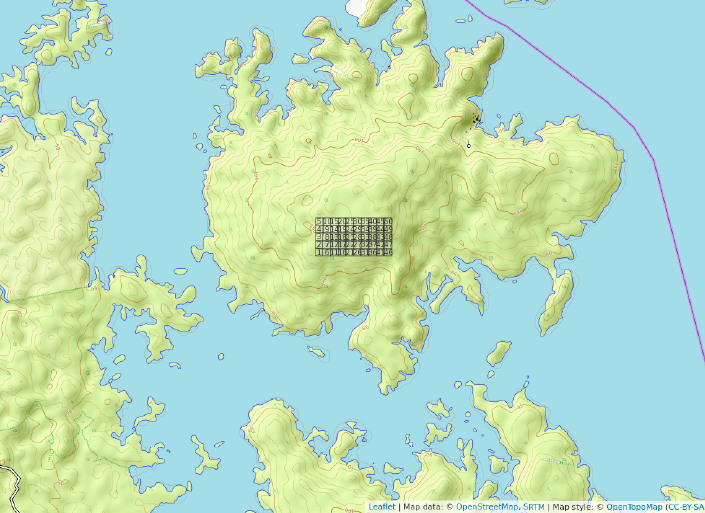
\includegraphics[width=0.50000\textwidth]{Mapa .png}
\caption{Área de estudio, parcela de 50ha, Isla Barro Colorado
\label{fig:Mapa}}
\end{figure}

\subsection{Materiales y Métodos}\label{materiales-y-muxe9todos}

La información de los cuadrantes que componen BCI fue procesada en R (R
Core Team, 2020), teniendo en cuenta la matriz ambiental y la matriz de
comunidad, los cuales contienen datos de las variables ambientales,
tales como condiciones edáficas, tipo de hábitat, topografía del lugar,
clasificación etaria del bosque, y datos demográficos y geoferenciación
espacial de todos los individuos censados. Se adaptaron scripts
reproducibles recuperados de Batlle (2020), utilizando la colección de
paquetes multifuncionales: vegan (Oksanen et al., 2019), Tidyverse
(Wickham, 2017), BiodiversityR (R. Kindt \& Coe, 2005) y indicspecies
(De Caceres \& Legendre, 2009).

Para conocer las características de los datos almacenados de la matriz
de comunidad y ambiental, se realizó un análisis exploratorio que
incluyó visualización de gráficos, tablas, mapas de los cuadrantes de
una hectárea y tablas de correlación lineal entre las dos variables de
la matriz, lo que permitió una vista común y ayudó a determinar
procedimientos más detallados a continuación.

\subsection{Medición de asociación
(ma)}\label{mediciuxf3n-de-asociaciuxf3n-ma}

Para realizar las pruebas de medición de asociación, se calculó la
distancia euclidiana entre los cuadrados considerados objetos. Para
ello, se requierió una transformación de la matriz de comunidad mediante
el método Hellinger, que incluye elevar al cuadrado la abundancia
relativa yij (cociente resultante de cada valor de abundancia entre la
suma de los sitios)(Legendre \& Gallagher, 2001). Además, se evaluó la
distancia euclidiana entre los cuadrantes en términos de ocurrencia de
especies. Se utilizó el índice de disimilitud de Jaccard de la matriz
normalizada para convertir el valor de abundancia en un valor binario
(Brocard, Gillet, \& Legendre, 2018). del mismo modo, se empleó la
métrica de Jaccard para aplicar la transposición de la matriz de la
comunidad y convertir a datos Presencia / ausencia para medir el grado
de asociación entre especies.

Para poder comparar la relación entre especies en función de su
abundancia, se utilizó estandarización \emph{ji}-cuadrado de la matriz
de comunidad transpuesta (Legendre \& Gallagher, 2001). Se examinó la
ocurrencia entre especies y su distribución en BCI por el coeficiente de
correlación entre rangos de Spearman, para medir el grado de correlación
entre las variables riqueza númerica de especies y la abundancia con las
variables ambientales geomorfológicas, y la composición química del
suelo (Brocard et al., 2018).

\subsection{Análisis de agrupamiento}\label{anuxe1lisis-de-agrupamiento}

El método jerárquico aglomerativo de asociación entre pares de
cuadrantes (según la composición de especies) bajo el estándar de enlace
completo, y el método de Ward basado en la varianza mínima, se utilizó
como método preliminar para el análisis de agrupamiento, con el fin de
probar su efectividad en lograr un grupo consistente de importancia
ecológica (Brocard et al., 2018). Luego, estos generaron dendrogramas
que posteriormente son comparados con la matriz de distancia de cuerdas
(Legendre \& Gallagher, 2001). Usando correlación cofenética entre los
dos para determinar el número ideal de grupos. Además, se utilizó
remuestreo bootstrap y boostrap multiescalar para conocer la
probabilidad de éxito de la inferencia del número de grupos y la
identidad de sus componentes (Brocard et al., 2018). Las distribuciones
se basaban en una probabilidad de 91\% o más de acierto para el método
bootstrap y de un 95\% para boostrap multiescalar.

Para conocer las especies distintas o asociadas a cada grupo, se utilizó
el valor del indicador o índice IndVal (``Conjuntos de especies y
especies indicadoras,'' 1997), basado en permutaciones aleatorias de los
sitios según la presencia de especies y la abundancia de estos. De
manera similar, el grado de asociación de una especie con una
preferencia particular por el grupo de cuadrantes considerado grupo en
estudio, expresado como el coeficiente de correlación biserial puntual
(Brocard et al., 2018). Se adoptó un enfoque similar al anterior a lo
largo de las pruebas estadísticas de la hipótesis nula, basada en las
especies presentes en los cuadrantes pertenecientes a un determinado
grupo realizado al azar. Esta prueba se hizo reordenando aleatoriamente
los valores de abundancia y comparando sus distribuciones con las
obtenidas previamente (Cáceres \& Legendre, 2009).

\subsection{Análisis de diversidad
alpha}\label{anuxe1lisis-de-diversidad-alpha}

La diversidad alpha representa la diversidad de especies a lo largo de
todas las subunidades locales relevantes, y por definición abarca dos
variables importantes: (1) la riqueza de especies, y (2) la abundancia
relativa de especies (Carmona-Galindo \& Carmona, 2013). Con el fin de
determinar la diversidad alpha se utilizaron métodos como la Entropia de
Shannon H1, que calcula el grado de desorden en la muestra, el índice de
concentración de Simpson, que calcula la probabilidad de que dos
individuos seleccionados aleatoriamente puedan ser de la misma especie.
Ademas, se empleó la serie de números de diversidad de Hill, la fórmula
de la entropía de Rengi y el índice de equidad de Pielou.

\subsection{Analisis de diversidad
beta}\label{analisis-de-diversidad-beta}

La diversidad beta, de acuerdo con (Whittaker, 1960), se define como el
diferencial entre la diversidad de un hábitat y la diversidad total de
un paisaje de hábitats. Teniendo en cuenta lo anterior, se utilizó el
metodo hellinger para determinar cuales son las especies que contribuyen
a la diversidad beta, es decir, las especies que no se encuentran
compartidas entre los cuadrantes.

\subsection{Análisis de ordenación simple (no restringida) y canónica
(restringida)}\label{anuxe1lisis-de-ordenaciuxf3n-simple-no-restringida-y-canuxf3nica-restringida}

Se aplicaron los análisis de componentes principales o PCA a los datos
de las variables ambientale para determianar la ordenación no
restringida, donde se tomó en cuenta especificamente las variables del
suelo. y para determinar la ordenacion restringida se exploró de manera
explícita las relaciones entre una matriz de respuesta y una matriz
explicativa con los análisis de redundancia o RDA, lo cual combina la
regresión y el análisis de componentes principales (PCA), por ejemplo,
busca tendencias en la matriz de comunidad restringiéndolas a la matriz
ambiental.

\subsection{Ecología espacial}\label{ecologuxeda-espacial}

En ecología espacial se utilizó la matriz transformada de hellinger y la
matriz ambiental para crear un cuadro de vecindad y ver como se
autocorrelacionan los sitios. Se genera un correlograma para la variable
que queremos estudiar mediante la función `sp.correlogram' y para varias
variables como la abundancia de especies y las variables ambientales.
También, se utilizaron otros métodos como la prueba Mantel con matrices
de distancia para autocorrelación espacial con y sin tendencia, y el I
de Moran con una matriz de abundancia de especies transformada sin
tendencia, lo cual se aplica a variables ambientales para obtener los
datos de autocorrelación, distribución de especies y variables en los
sitios de muestreo.

\section{Resultados}\label{resultados}

Se registraron un total de 5 especies y 2 generos distribuidos en 2029
individuos en toda la parcela. La riqueza por cuadro fue de 4 especies y
la mediana de la abundancia por cuadro fue de 39 individuos. La especie
más abundante fue \emph{Pouteria reticulata}, con 1084 individuos, y la
menos abundante fue \emph{Pouteria fossicola} con 3 individuos. La tabla
\ref{tab:abun_sp} y la figura \ref{fig:abun_sp_q} resume estos
resultados. La distribución de la riqueza númerica de especies de la
familia Sapotaceae sigue un patrón homogeneo, lo cual los agregados de
riqueza máxima están distribuidos en casi todo el área (ver Figura
\ref{fig:mapa_cuadros_riq_mi_familia}). Cabe resaltar, que la
distribución de las variables ambientales PH y pendiente media siguen un
patrón relativamente similar a la distribución de la riqueza númerica de
la familia Sapotaceae.

\begin{longtable}[]{@{}lr@{}}
\caption{\label{tab:abun_sp}Abundancia por especie de la familia
Sapotaceae}\tabularnewline
\toprule
Latin & n\tabularnewline
\midrule
\endfirsthead
\toprule
Latin & n\tabularnewline
\midrule
\endhead
Pouteria reticulata & 1084\tabularnewline
Chrysophyllum argenteum & 711\tabularnewline
Chrysophyllum cainito & 171\tabularnewline
Pouteria stipitata & 60\tabularnewline
Pouteria fossicola & 3\tabularnewline
\bottomrule
\end{longtable}

\begin{figure}
\centering
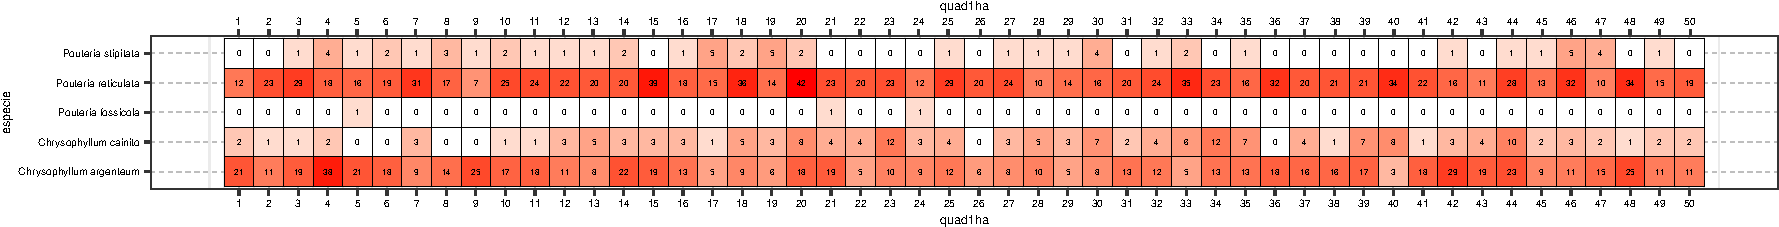
\includegraphics{manuscrito_files/figure-latex/unnamed-chunk-3-1.pdf}
\caption{\label{fig:abun_sp_q}Abundancia por especie por quadrat}
\end{figure}

\begin{figure}
\centering
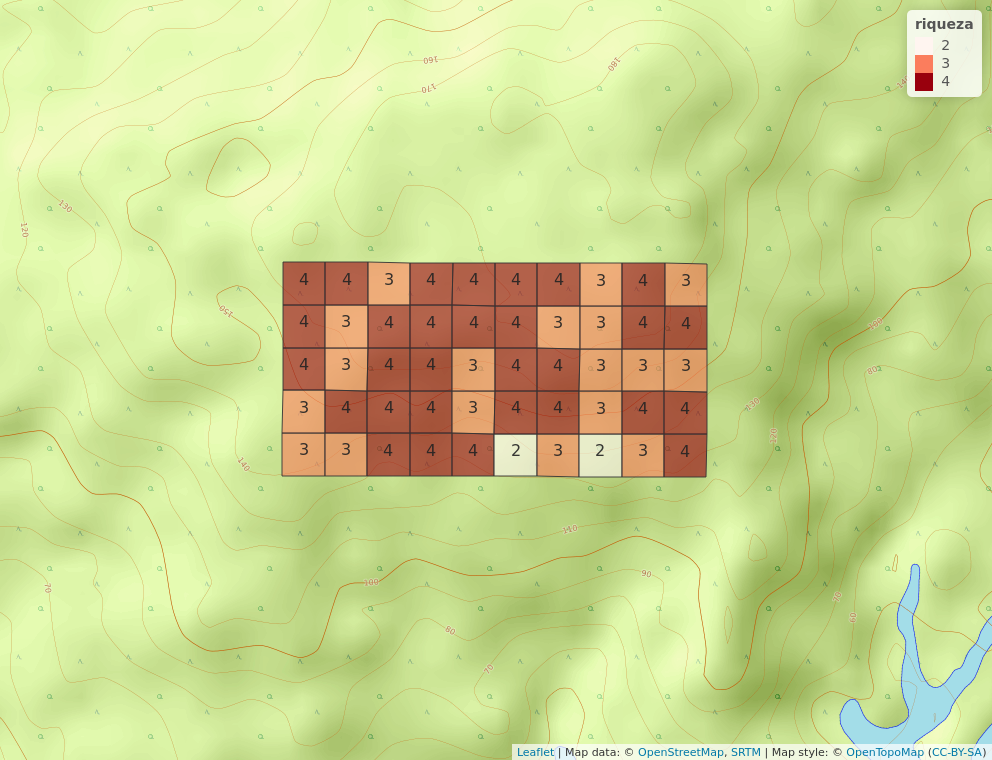
\includegraphics[width=0.50000\textwidth]{mapa_cuadros_riq_mi_familia.png}
\caption{Distribucion de la riqueza de la familia
Sapotaceae\label{fig:mapa_cuadros_riq_mi_familia}}
\end{figure}

Los valores para el coeficiente de Spearman presentados en el panel de
correlación de la figura \ref{fig:p_cor_suelo_ar}, mostraron que la
abundancia de la familia sapotaceae solo presenta correlación con la
abundacia global, mientras que la riqueza tiene correlación con la
presencia de cobre y nitrógeno en el suelo, lo que sugiere que mientras
mas concentración de cobre y nitrógeno hay, mayor será la riqueza de
especies.

\begin{figure}
\centering
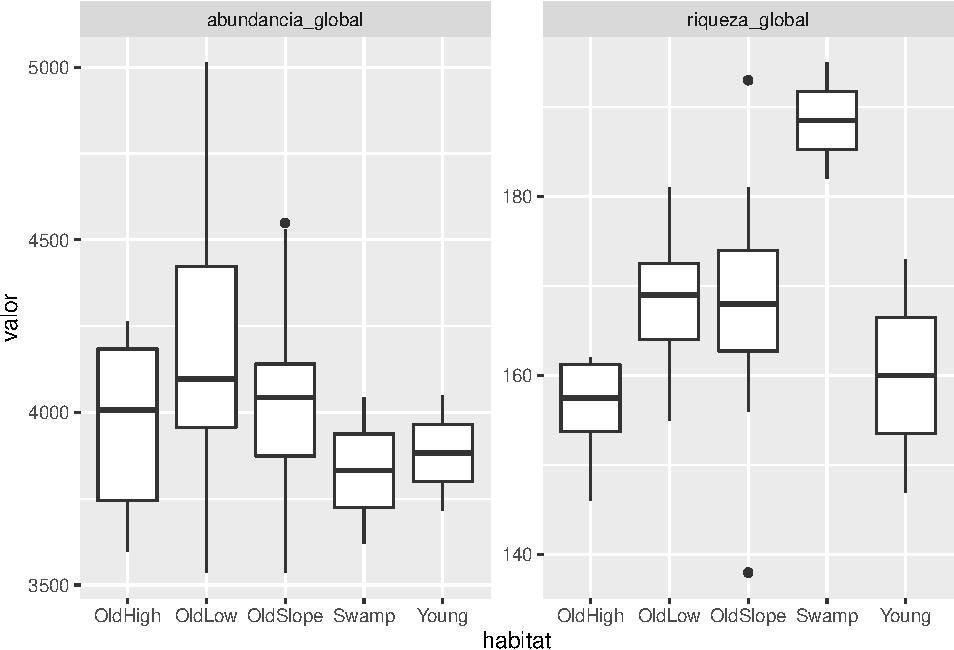
\includegraphics{manuscrito_files/figure-latex/unnamed-chunk-4-1.pdf}
\caption{\label{fig:p_cor_suelo_ar}correlacion de las variables del
suelo}
\end{figure}

El índice de similaridad de Jaccard muestra que el sitio 1 y 2 comparten
un 100\% de sus especies, por lo que ambos sitios comparten 3 especies y
no tienen especies exclusivas (ver figura
\ref{fig:similaridad_jaccard}). Las variables geomorfológicas presentan
asociación con la abundancia y riqueza, lo cual la figura
\ref{fig:matriz_correlacion_geomorf_abun_riq_spearman} muestra que hay
mucha similaridad entre estas variables. Las pruebas de correlación
entre los grupos 1 y 2 formulados por upgma resultaron significativas
respecto a la variable fósforo. Por otro lado, el contenido de cobre y
la abundancia global promedio, es decir, la media correspondiente a
todas las plantas en BCI, son significativamente diferentes entre los
sitios de ambos grupos, para un nivel de significancia de a = 0.1(ver
figura \ref{fig:grupos_upgma}).

El grupo 1 generado por enlace upgm esta conformado por 5 cuadrante y el
grupo 2 por 46 cuadrantes (ver figura \ref{fig:mapa_upgma_k2}). El grupo
2 contiene los sitios con tendencia a presentar valores altos de zinc y
contenido de cobre. Es probable que las especies indicadoras del grupo
con un mayor contenido de cobre estén mostrando preferencia por estas
condiciones ambientales. No obstante, la mayoría de componentes del
suelo en BCI tienen valores bastante homogéneos, y más bien se presentan
pequeños gradientes entre los cuadrantes, lo cual evita que este tipo de
acercamiento sea concluyente. La especie \emph{Chrysophyllum argenteum}
fué la que obtuvo un valor alto de confianza al examinar su potencial
como especies indicadoras del grupo 1. Para el caso del grupo 2, la
especie indicadora fué \emph{Pouteria reticulata}.

\begin{figure}
\centering
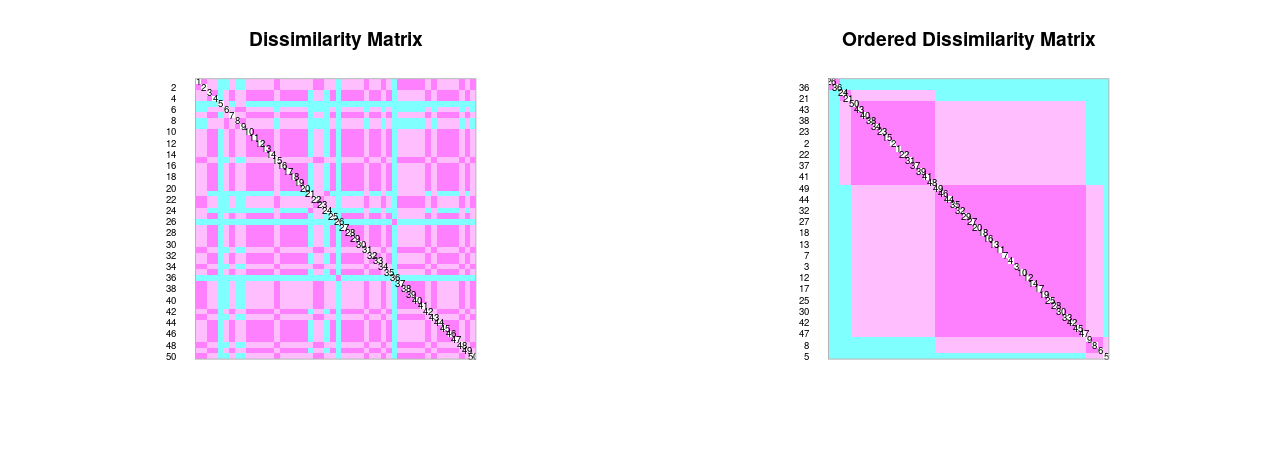
\includegraphics[width=1.00000\textwidth]{Similaridad.png}
\caption{Similaridad de Jaccard (color fucsia (magenta, rosa) significa
``corta distancia=muy similares'', y cian (celeste) significa ``gran
distancia=poco similares'')\label{fig:similaridad_jaccard}}
\end{figure}

\begin{figure}
\centering
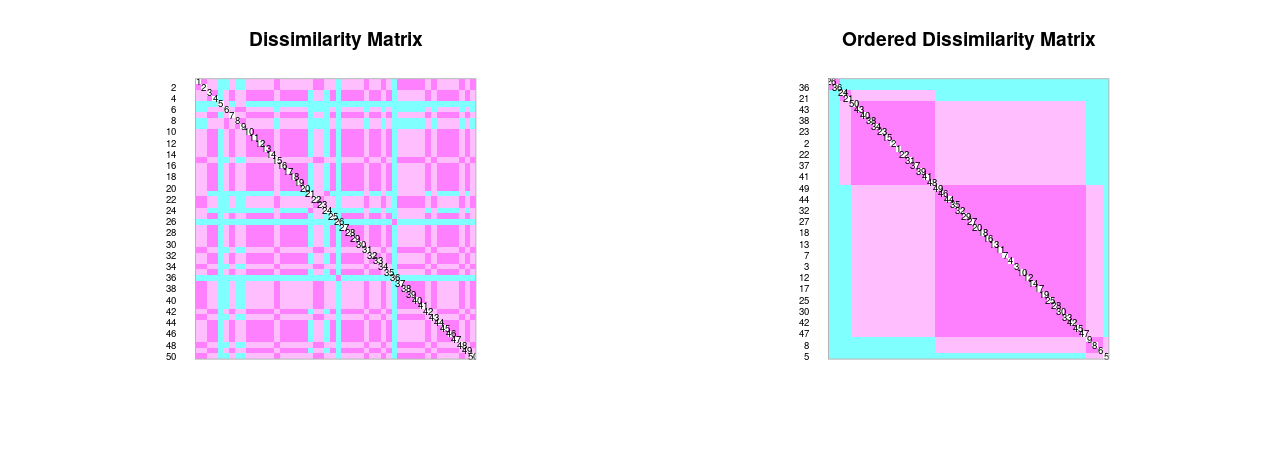
\includegraphics[width=1.00000\textwidth]{Similaridad.png}
\caption{Panel de correlacion de Spearman entre los datos de la
comunidad y las variables geomorfologicas (color fucsia (magenta, rosa)
significa ``corta distancia=muy similares'', y cian (celeste) significa
``gran distancia=poco
similares'')\label{fig:matriz_correlacion_geomorf_abun_riq_spearman}}
\end{figure}

\begin{figure}
\centering
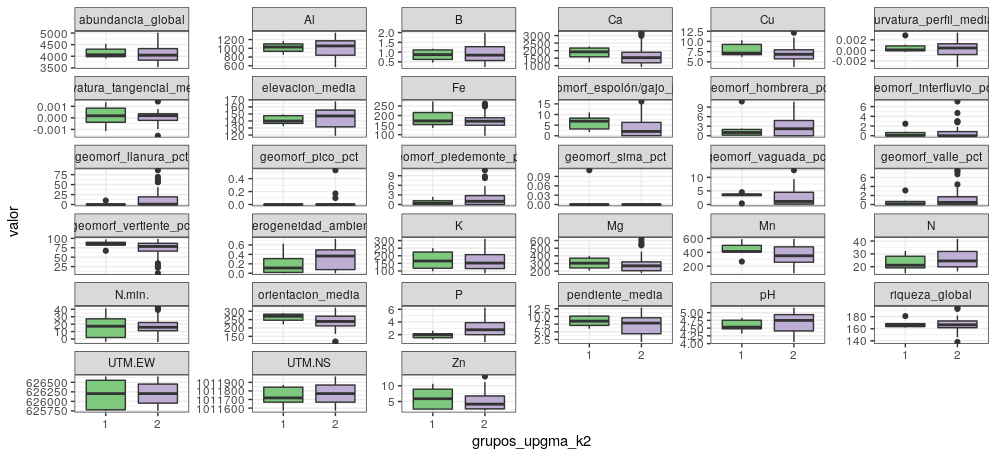
\includegraphics[width=1.00000\textwidth]{actualizacion2_grupos_upgma.png}
\caption{Diagramas de caja de las variables que tuvieron un efecto,
segun las pruebas de igualdad de medias\label{fig:grupos_upgma}}
\end{figure}

\begin{figure}
\centering
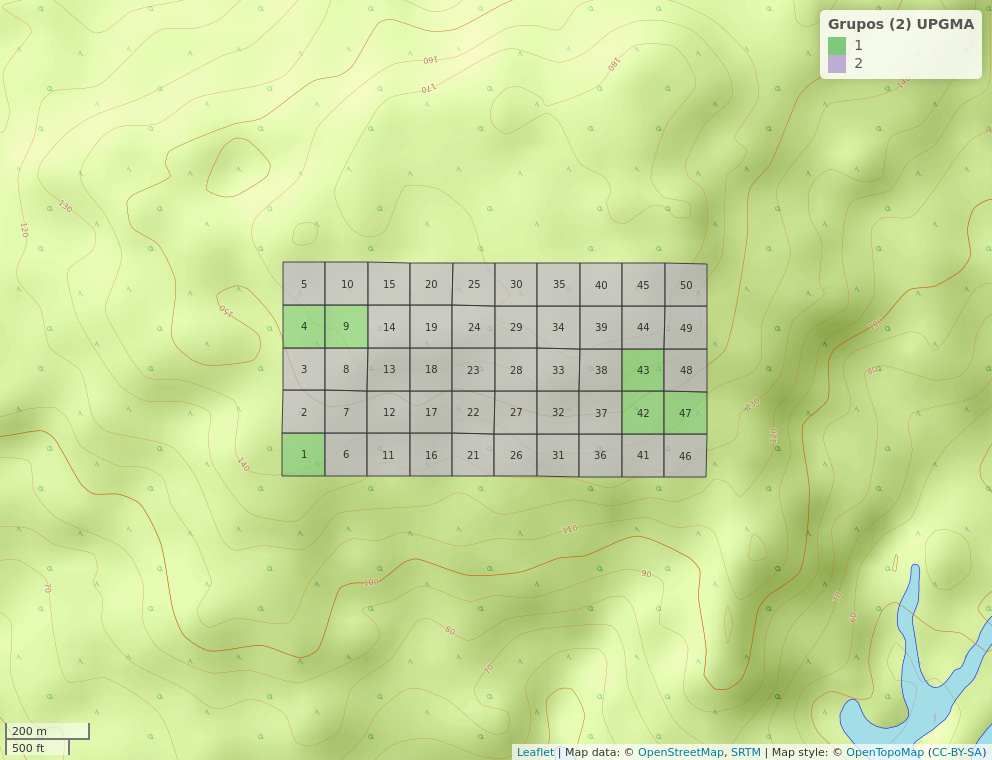
\includegraphics[width=0.50000\textwidth]{mapa_upgma_k2.png}
\caption{Mapa en el que se presenta la distribución de sitios en los
grupos formulados por enlace upgma\label{fig:mapa_upgma_k2}}
\end{figure}

La riqueza de la familia Sapotaceae aumenta en función del contenido de
hidrógeno, nitrógeno y cobre, ademas, aunmenta con la equidad. Cabe
destacar, que algunos sitios de BCI tienen valores altos de equidad (ver
figura \ref{fig:grafico_niveles_equidad}). La Curva de rarefacción de
los sitios, muestra como va aumentando la cantidad de individuos y de
especies de los cuadrantes (ver figura \ref{fig:Curva_rarefaccion}),
donde la mayor concentración de individuos está entre los 20 a 50
individuos y la abundancia maxima es de 70 individuos. Los valores de
los indices de diversidad alfa fueron: Riqueza de especies (0.22),
Shannon (0.05) y Simpson (0.04).

\begin{figure}
\centering
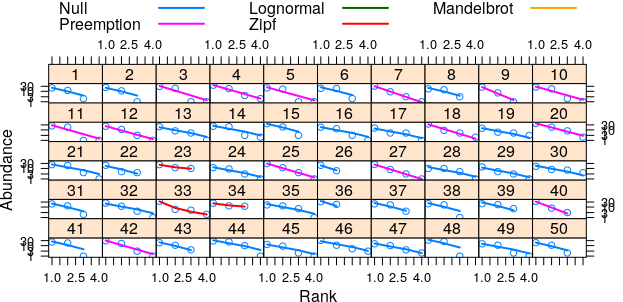
\includegraphics{grafico_niveles_equidad.png}
\caption{Grafico dque presenta los valores de equidad por sitos
\label{fig:grafico_niveles_equidad}}
\end{figure}

\begin{figure}
\centering
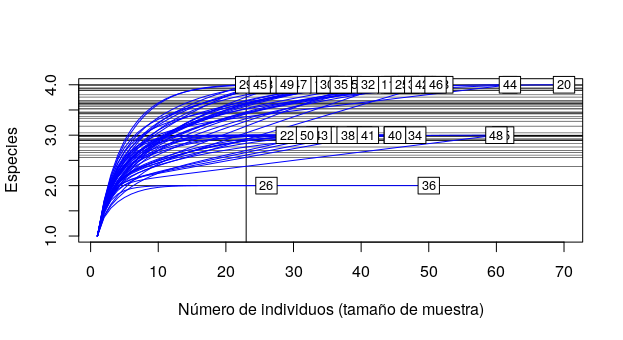
\includegraphics{Curva_rarefaccion.png}
\caption{Curva de rarefaccion de los sitios
\label{fig:Curva_rarefaccion}}
\end{figure}

Las especies que contribuyen de manera significativa a la diversidad
beta fueron: \emph{Chrysophyllum argenteum} (0.25), \emph{Chrysophyllum
cainito} (0.31) y \emph{Pouteria stipitata} (0.27), de las cuales la que
mas contribuyó fué \emph{Chrysophyllum cainito}. No obstante, los sitios
que contribuyen a la diversidad beta son los cuadrantes 9 y 40, lo cual
presentan contribución debido a la incidencia de algunas variables
ambientales.

El gráfico \ref{fig:env_suelo_pca} incluye el comportamiento de los
componentes principales de la varianza en las variables suelo y
geomorfología en BCI, predecido por el modelo de barra quebrada,
representado por la línea roja formando la curva (La escala denominada
``Inertia'' representa la suma de los cuadrados de toda la varianza). En
el diagrama rotulado como escalamiento 1 de la figura
\ref{fig:Biplot_PCA_escalamiento}, se observan tres grupos de cuadrantes
diferenciados entre sí. Un grupo de sitios con un alto grado de acidez y
contenido en aluminio, otro grupo caracterizado por la presencia de
elementos metálicos, y un tercero, con una cantidad de fósforo,
nitrógeno y valor de pH mayor. Las variables nitrógeno, fósforo y pH
aportan la mayor parte de la varianza explicada. La relación entre las
variables se encuentra debidamente representada en el recuadro del
escalamiento 2, por medio de los ángulos que forman sus vectores (ver
figura \ref{fig:Biplot_PCA_escalamiento}). Los resultados del PCA de los
datos de la matriz de comunidad se encuentran resumidos en los diagramas
de la figura \ref{fig:PCA_comunidad}. El escalamiento 1, muestra muchos
de los cuadrantes dispuestos alrededor del origen formado por los ejes,
lo que indica una contribución a la varianza relativamente equitativa
por parte de las especies.

\begin{figure}
\centering
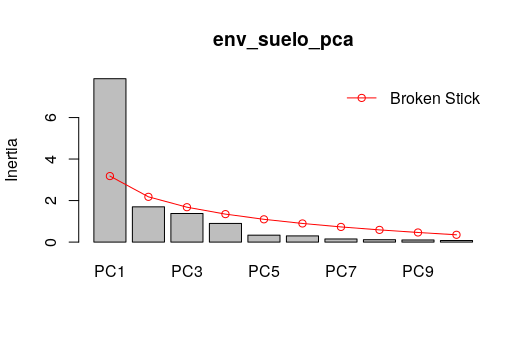
\includegraphics{env_suelo_pca.png}
\caption{grafico de los componentes principales de la varianza en las
variables suelo y geomorfologia en BCI \label{fig:env_suelo_pca}}
\end{figure}

\begin{figure}
\centering
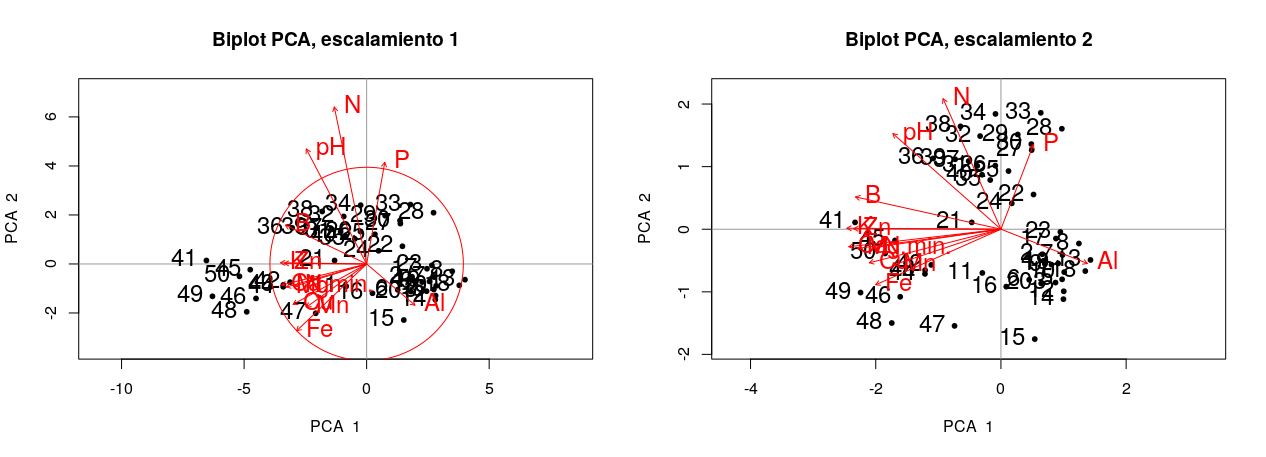
\includegraphics[width=1.00000\textwidth]{Biplot_PCA_escalamiento_actualizado.png}
\caption{Biplots generados en el PCA de las viariables de suelo
\label{fig:Biplot_PCA_escalamiento}}
\end{figure}

\begin{figure}
\centering
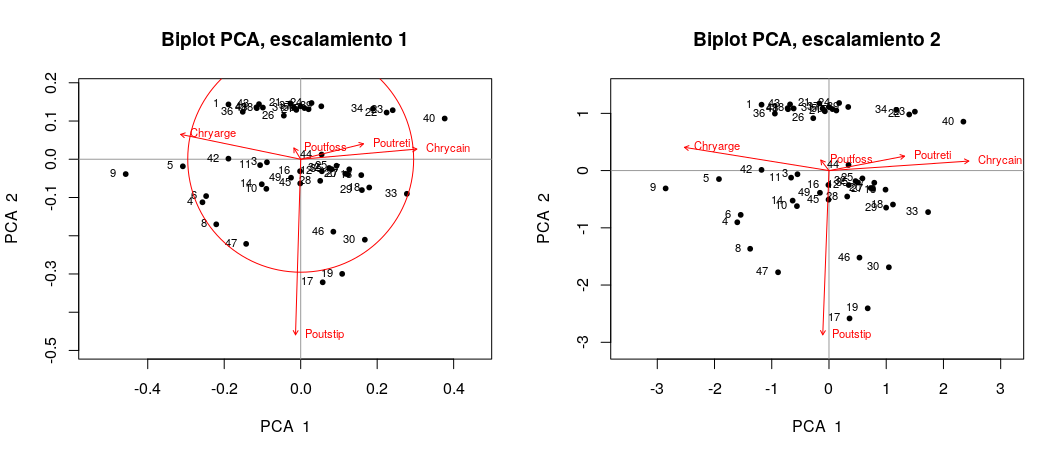
\includegraphics[width=1.00000\textwidth]{PCA_comunidad_actualizado.png}
\caption{Biplots generados en el PCA de las viariables de suelo
\label{fig:PCA_comunidad}}
\end{figure}

El escalamiento 2 de la figura \ref{fig:Analisis_de_correspondencia} en
el análisis de correspondencia mostró que las especies \emph{Pouteria
reticulata}, \emph{Chrysophyllum argenteum} y \emph{Chrysophyllum
cainito} se encuentran asociadas. Las especies restantes tienen una
abundancia reducida, y en consecuencia, aparecen cercanas a los pocos
cuadrantes en los que se encuentran representadas. La disparidad en la
incidencia de las especies se refleja en su disposición en el diagrama.
Sin embargo, estos resultados no coinciden del todo con los arrojados
por el PCA de la matriz de distancias.

Los primero ordenes de \emph{Chrysophyllum argenteum} y
\emph{Chrysophyllum cainito} presentan valores de autocorrelación alta o
positiva, mientras que los ordenes de las demas especies presentan
mayormente valores de autocorrelación negativa (Ver figura
\ref{fig:Abundancia_matriz}).

\begin{figure}
\centering
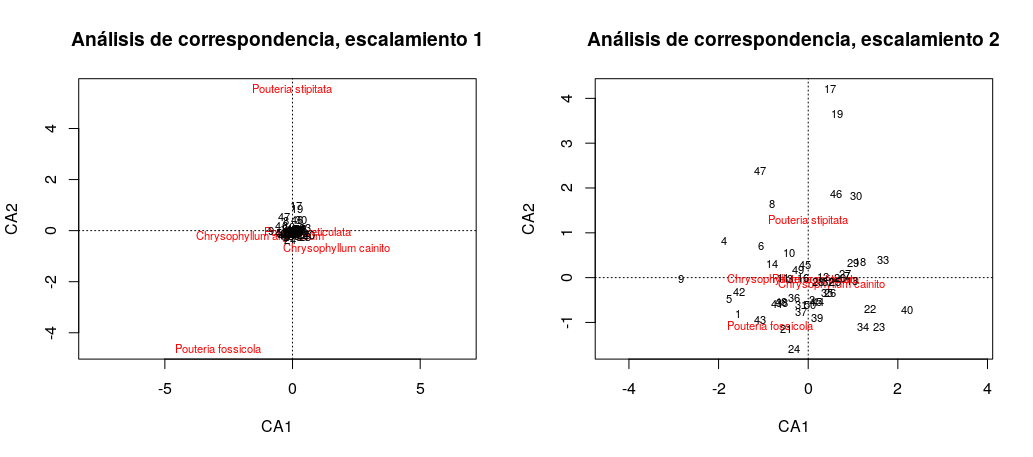
\includegraphics[width=1.00000\textwidth]{analisis_de_correspondencia_actualizado.png}
\caption{Biplot del analisis de correspondencia de los datos de
abundancia de las especies de Sapotaceae
\label{fig:Analisis_de_correspondencia}}
\end{figure}

\begin{figure}
\centering
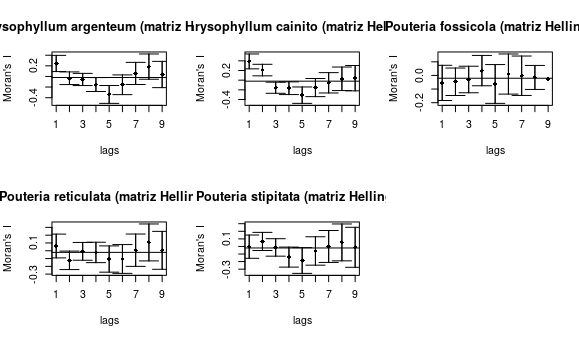
\includegraphics[width=1.00000\textwidth]{Abundancia_matriz.png}
\caption{Autocorrelación espacial de las especies
\label{fig:Abundancia_matriz}}
\end{figure}

\section{Discusión}\label{discusiuxf3n}

Estudios de la familia Sapotaceae también reportan que \emph{Pouteria}
es un género que parece siempre presentar una cantidad significativa de
individuos (Martínez-Sovero et al., 2021). La riqueza de la familia
Sapotaceae aumenta en función del contenido de hidrógeno, nitrógeno y
cobre, los cuales son algunos de los nutrientes que más se correlacionan
con la diversidad de especies de plantas en el neotrópico (Doblado
Amador, 2011). Ademas, la riqueza aunmenta con la equidad, debido a que
las especies estan distribuidas en casi todos los cuadrantes.

Los valores de los indices de diversidad alfa fueron muy bajos, por
consiguiente, la familia Sapotaceae no presenta mucha diversidad en BCI.
Se estima que la riqueza seguiría constante o no aumentaría
significativamente aunque se hiciera mayor esfuerzo de muestreo (ver
figura \ref{fig:acumulacion_especies_individuos}).

\begin{figure}
\centering
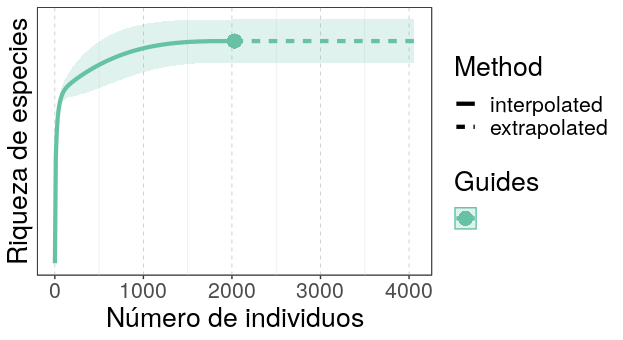
\includegraphics{acumulacion_especies_individuos.png}
\caption{Grafico de acumulacion de especies en funcion de numeros de
individuos \label{fig:acumulacion_especies_individuos}}
\end{figure}

Las especies que contribuyen de manera significativa a la diversidad
beta fueron: \emph{Chrysophyllum argenteum}, \emph{Chrysophyllum
cainito} y \emph{Pouteria stipitata}, las cuales fueron las que
obtuvieron valores intermedios de individuos. No obstante, los sitios
que contribuyen a la diversidad beta son los cuadrantes 9 y 40, ya
presentan contribución por la incidencia de algunas variables
ambientales, tales como PH, aluminio, boro, manganeso, etc. Lo anterior
coincide con (Horvát et al., 2010), lo cual explica que la distribución
de la abundancia relativa se ve afectada por interacciones, que en este
caso se debe a la incidencia de algunas variables ambientales. Además,
(R. Condit et al., 2002) señala que la diversidad beta aumenta
dependiendo la distancia que estan separadas las especies o los sitios
donde se encuentran estas.

Las especies \emph{Pouteria reticulata}, \emph{Chrysophyllum argenteum}
y \emph{Chrysophyllum cainito} se encuentran asociadas, debido a que
tienen los valores mas altos de abundancia dentro de la comunidad (1084,
711 y 171 individuos, respectivamente). Finalmente, los primeros ordenes
de \emph{Chrysophyllum argenteum} y \emph{Chrysophyllum cainito}
presentan valores de autocorrelación positiva, mientras que los ordenes
de las demás especies presentan mayormente valores de autocorrelación
negativa, teniendo en cuenta que el orden 5 de todas las especies
presenta autocorrelacion negativa, lo que sugiere que el orden 5 de las
especies está autocorrelacionado espacialmente negativo.

\section{Agradecimientos}\label{agradecimientos}

Agradezco al maestro José Ramón Martinez, por su motivación y ayuda en
todos los aspectos para que este trabajo salga bien.

\section{Información de soporte}\label{informaciuxf3n-de-soporte}

\ldots

\section{\texorpdfstring{\emph{Script}
reproducible}{Script reproducible}}\label{script-reproducible}

\subsection{Análisis de riqueza y
abundancia}\label{anuxe1lisis-de-riqueza-y-abundancia}

\begin{verbatim}

#' ---
#' title: "Análisis exploratorio de datos. Riqueza y abundancia"
#' author: "JR"
#' date: "13 de octubre, 2020"
#' output: github_document
#' ---

#' ### Área de cargar paquetes
library(vegan)
library(tidyverse)
library(sf)
source('biodata/funciones.R')

#' ### Área de cargar datos
#' Censo (el objeto se carga con prefijo "censo") y matriz de comunidad (prefijo "mc")
load('biodata/Sapotaceae.Rdata')
load('biodata/matriz_ambiental.Rdata') #Matriz ambiental, se carga como "bci_env_grid"

#' ### Imprimir datos en pantalla (impresiones parciales con head)
head(censo_saptc)
head(mc_saptc)
bci_env_grid # No necesita imprimirse parcialmente

#' ### También podemos usar
#' Requiere que se haya cargado ya la colección tidyverse
censo_saptc %>% tibble
mc_saptc %>% tibble

#' ### Lista de especies
sort(colnames(mc_saptc))

#' ### Número de sitios, tanto en matriz de comunidad como en ambiental
#' Verifica que coinciden
nrow(mc_saptc) #En la matriz de comunidad
nrow(bci_env_grid) #En la matriz ambiental

#' ### Riqueza numérica de especies (usando matriz de comunidad) por quadrat
#' Nota: cargar paquete vegan arriba, en el área de paquetes
specnumber(mc_saptc)
sort(specnumber(mc_saptc)) # Ordenados ascendentemente
summary(specnumber(mc_saptc)) # Resumen estadístico

#' ### Abundancia de especies por quadrat
sort(rowSums(mc_saptc))
summary(rowSums(mc_saptc)) # Resumen estadístico

#' ### Abundancia por especie
sort(colSums(mc_saptc))
summary(colSums(mc_saptc)) # Resumen estadístico

#' ### Riqueza numérica de toda la "comunidad"
specnumber(colSums(mc_saptc))

#' ### Abundancia de toda la comunidad
sum(colSums(mc_saptc))

#' ### Una tabla para el manuscrito, es necesario asignarle nombre
#' Para esto, usaré la colección "tidyverse"
abun_sp <- censo_saptc %>%
  group_by(Latin) %>% 
  count() %>% 
  arrange(desc(n))
abun_sp

#' ### Un gráfico para el manuscrito
#' Gráfico de mosaicos de la abundancia por especie por cuadros
abun_sp_q <- crear_grafico_mosaico_de_mc(mc_saptc, tam_rotulo = 12)
abun_sp_q
\end{verbatim}

\subsection{Análisis con la colección
tidyverse}\label{anuxe1lisis-con-la-colecciuxf3n-tidyverse}

\begin{verbatim}

#' ---
#' title: "Análisis exploratorio de datos. Colección tidyverse"
#' author: "JR"
#' date: "18 de octubre, 2020"
#' output: github_document
#' ---

#' # ¿Qué es tidyverse?
#' 
#' Es una colección de paquetes con los que podrás importar, transformar, visualizar, modelar y presentar datos. La colección se compone de 8 paquetes, de los cuales verás sobre todo 3: `dplyr`, `tidyr` y `ggplot2`.
#' 
#' Todos estos paquetes comparten estructuras comunes. Una de las herramientas que incorpora la colección es la pipa `%>%` (**SHORTCUT: `CTRL+SHIFT+M`**), la cual importa desde el paquete `magrittr`. Usarás la pipa para construir "tuberías" de procesamiento sin necesidad de crear objetos intermedios. En una tubería, puedes interpretar la pipa como **"luego"**, y verás más adelante por qué. La función principal de la pipa (tiene muchas, pero esta es la más importante) es pasar el resultado del objeto a su izquierda como primer argumento de la función a su derecha. El siguiente ejemplo explica su uso:
#' 
#' `objeto1 %>% funcion1()` es equivalente a `funcion1(argumento1 = objeto1)`
#' 
#' > La idea del *pipe* pertenece a la tradición de sistemas tipo Unix y, en origen, su función era comunicar distintos procesos, usando la salida estándar de uno (*stdout*) como entrada estándar (*stdin*) del siguiente.
#' 
#' Su ventaja radica en que, si necesitaras continuar procesando los datos, no tendrás que anidar ni crear objetos intermedios. En el siguiente ejemplo, asigno el resultado de una cadena al objeto nombrado `resultado`:
#' 
#' `resultado <- objeto1 %>% funcion1() %>% funcion2() %>% funcion3()`
#' 
#' Puedes leer lo anterior como *"objeto1 pasa como primer argumento de funcion1, **luego** el resultado de funcion1 pasa como primer argumento de funcion2, **luego** el resultado de funcion2 pasa como primer argumento de funcion3*.
#' 
#' Para replicar esta operación sin la pipa, podrías realizarlo de, por ejemplo, dos maneras distintas:
#' 
#' * Opción 1, anidar:
#' 
#' `resultado <- funcion3(funcion2(funcion1(objeto1)))`
#' 
#' Opción 2, crear objetos intermedios:
#' 
#' `tmp1 <- funcion1(objeto1)`
#' `tmp2 <- funcion2(tmp1)`
#' `resultado <- funcion3(tmp2)`
#' 
#' Notarás que, comparada con estas dos últimas opciones, la tubería es más limpia que estas dos últimas opciones. La tubería puedes leerla de forma encandenada, a diferencia del estilo anidado y de creación de objetos intermedios, que añade una cierta complejidad de lectura para el usuario/a, sobre todo para personas sin conocimientos de programación. Precisamente por esta razón fue que decidí introducir la colección tidyverse, para así mostrarte algunas ideas que podrás aplicar a tus datos y, en principio, para facilitarte la vida ("*no me ayude' tali*"). Ahora bien, si decides programar en R más adelante, deberás aprender las capacidades de programación orientada a objetos y programación funcional de R.
#' 
#' ¡Comencemos!
#' 
#' ## Paquetes
#' 
library(tidyverse)
library(sf)
#' 
#' > `sf` te ayudará a leer el objeto `bci_env_grid` como un *simple feature*, el cual se encuentra dentro del archivo `biodata/matriz_ambiental.Rdata`. Esto extenderá las capacidades espaciales del objeto.
#' 
#' ## Cargar datos
#' 
load('biodata/matriz_ambiental.Rdata')
load('biodata/Sapotaceae.Rdata')
#'  
#' ## Paquete `dplyr`
#' 
#' Te servirá para manipular datos mediante verbos. Los verbos de `dplyr` que conocerás son (hay muchos otros): `select()`, `filter()`, `arrange()`, `mutate()`, `group_by()`, `summarise()` y `join`.
#' 
#' ### Verbo `select`
#' 
#' Comúnmente, necesitas seleccionar una o varias columnas de una tabla. Para esto existe el verbo `select`. Te muestro un ejemplo aplicado a la matriz de comunidad (que por ahora la verás como `simple feature`), seleccionando las columnas `id` (número identificador de quadrat) y `pH` (pH del suelo):
bci_env_grid %>%
  select(id, pH)
#' > Importante: el objeto `bci_env_grid` permanece intacto, a menos que se use dicho nombre para reasignarlo a otro objeto. Mientras no se use el asignador `<-`, sólo verás que manipulo y visualizo copias del objeto original.
#' Fíjate en la clase del objeto `bci_env_grid`. Para ello usaré la función de R `class`. No sólo se admiten verbos `dplyr`, cualquier función puede usarse:
bci_env_grid %>%
  class
#' El objeto `bci_env_grid` es a la vez de clase `sf` (*simple feature*) y `data.frame`, es decir, es tanto tabla como objeto espacial, por lo que se puede representar en un mapa. Este objeto no pierde la clase `sf`, por lo que verás que aparece información geométrica y geoespacial en el encabezado, y luego un extracto de la tabla de datos (como máximo, las 10 primeras filas). Para convertirlo a un simple `data.frame`, hay que "tumbar" su geometría con `st_drop_geometry`:
bci_env_grid %>%
  select(id, pH) %>%
  st_drop_geometry
#' Fíjate ahora en la clase de `bci_env_grid %>% select(id, pH) %>% st_drop_geometry`, que en este caso es sólo `data.frame`:
bci_env_grid %>%
  select(id, pH) %>%
  st_drop_geometry %>%
  class
#' > Al introducir un `<enter>` después de la pipa, el código puede continuar en la línea siguiente. Esto se hace para evitar que la línea de código sea legible sin necesidad de desplazarse hacia la derecha (es aconsejable no superar los 80 caracteres en una misma línea de código, según recomiendan en la [Google’s R Style Guide](https://google.github.io/styleguide/Rguide.html)). Como convención, escribiré un `<enter>` después de cada operador pipa.
#' 
#' Seleccionaré, y a la vez renombraré, dos columnas con `select` (recuerda: no estoy modificando el objeto original, simplemente trabajo en copias no asignadas). De paso, sólo mostraré las 6 primeras filas al aplicar `head` al final de la tubería (no sólo se admiten verbos `dplyr`, cualquier función de R puede entrar en la tubería):
bci_env_grid %>%
  select(id_de_quadrat = id, pH_del_suelo = pH) %>%
  st_drop_geometry %>%
  head
#' 
#' Otra funcionalidad de `select` es poder seleccionar columnas según patrones. Por ejemplo, si quisera seleccionar únicamente las variables sobre geomorfología (todas las columnas que comienzan por `geomorf`), podría hacerlo con relativa facilidad usando la función de ayuda `contains`
#' 
bci_env_grid %>%
  select(contains('geomorf')) %>%
  st_drop_geometry
#' ...y también usando expresiones regulares con `matches`, usando por ejemplo dos cadenas de caracteres...
bci_env_grid %>%
  select(matches('geomorf|habit', ignore.case = F)) %>%
  st_drop_geometry
#' ...o pidiendo todas las columnas que comienzan por mayúsculas, excepto las que comienzan por "U", lo cual excluye las coordenadas (e.g. `UTM.NS`), y deja sólo los elementos de análisis de suelo.
bci_env_grid %>%
  select(matches('^[A-T,Z]', ignore.case = F)) %>%
  st_drop_geometry
#' ### Verbo `filter`
#' 
#' Ahora mostraré sólo los elementos con `pH` mayor que 5, usando el verbo `filter`
bci_env_grid %>%
  select(id, pH) %>%
  st_drop_geometry %>%
  filter(pH>5)
#' O filtro por aquellos con `id` 31 y 50:
bci_env_grid %>%
  select(id, pH) %>%
  st_drop_geometry %>%
  filter(id == c(31, 50))
#' 
#' ### Verbo `arrange`
#' 
#' Pruebo también con la matriz de comunidad. Por ejemplo, introduzco en la tubería la función `colSums`, que devuelve un vector cuyos elementos están nombrados (tienen un atributo, en este caso, el nombre de especie), donde cada elemento representa la abundancia por especie.
mc_saptc %>%
  colSums
#' Y también obtengo la abundancia por quadrat.
mc_saptc %>%
  rowSums
#' Uso a continuación el verbo `arrange` para mostrar los registros de la matriz ambiental ordenados ascendentemente por pH.
bci_env_grid %>%
  select(id, pH) %>%
  st_drop_geometry %>%
  arrange(pH)
#' Ahora usaré `arrange` para mostrar los registros de la matriz ambiental ordenados DESCendentemente por pH.
bci_env_grid %>%
  select(id, pH) %>%
  st_drop_geometry %>%
  arrange(desc(pH))
#' 
#' ### Verbo `mutate`
#' 
#' Usaré el verbo `mutate` para crear una nueva columna. Por ejemplo, creo una columna que contenga `habitat` y `quebrada` separadas por una coma:
bci_env_grid %>%
  st_drop_geometry %>%
  select(habitat, quebrada) %>% 
  mutate(habitat_quebrada = paste(habitat, quebrada, sep = ', '))
#' Ahora `mutate`, pero con números: creo una columna de área de cada cuadro (necesitas también la función `st_area`, del paquete `sf`):
bci_env_grid %>%
  mutate(area = st_area(geometry)) %>%
  select(id, area) %>%
  st_drop_geometry %>%
  head
#' ...y ahora más complejo: obtengo la densidad de individuos por metro cuadrado, ordenados descendentemente por dicha densidad, y conservando sólo los 6 registros con mayores densidades.
bci_env_grid %>%
  mutate(area = st_area(geometry), densidad_indiv = abundancia_global/area) %>% 
  select(id, densidad_indiv) %>% 
  st_drop_geometry %>% 
  arrange(desc(densidad_indiv)) %>% 
  head
#' 
#' ### Verbos `group_by` y `summarise`
#' 
#' Los verbos `group_by` y `summarise` son útiles para producir resúmenes por grupos.
#' 
#' Agruparé la matriz ambiental por la columna `habitat`, dejando sólo las variables numericas que hagan sentido (por ejemplo, excluyo `id`, `UTM.EW`, `UTM.NS`), y lo asignaré a `agrupado_por_habitat` para luego reutilizarlo:
agrupado_por_habitat <- bci_env_grid %>%
  st_drop_geometry %>%
  group_by(habitat) %>% 
  select_if(is.numeric) %>%
  select(-id, -UTM.EW, -UTM.NS)
agrupado_por_habitat
#' Observa el encabezado: el objeto es `A tibble: 50 x 32` y hay 5 grupos (`Groups:   habitat [5]`). Calculo cuántos elementos (filas) hay por grupo:
agrupado_por_habitat %>% summarise(n = n())
#' ...y también algunos estadísticos de las columnas `pH`, `abundancia_global` y `riqueza_global` por ejemplo:
agrupado_por_habitat %>%
  summarise(
    n = n(),
    media_pH = mean(pH),
    media_abundancia = mean(abundancia_global),
    media_riqueza = mean(riqueza_global)
  )
#' ...o la media de todas las variables numéricas
agrupado_por_habitat %>%
  summarise_all(mean)
#' ...no caben, mejor por partes
agrupado_por_habitat %>%
  summarise_all(mean) %>% 
  select(1:6) %>% 
  print(width=300)
agrupado_por_habitat %>%
  summarise_all(mean) %>% 
  select(1,7:12) %>% 
  print(width=300)
agrupado_por_habitat %>%
  summarise_all(mean) %>% 
  select(1, 13:25) %>% 
  print(width=300)
agrupado_por_habitat %>%
  summarise_all(mean) %>% 
  select(1, 26:32) %>%
  print(width=300)
#' ...y no sólo un estadístico, sino varios:
agrupado_por_habitat %>%
  summarise_all(
    list(
      media = mean,
      mediana = median,
      varianza = var,
      minimo = min,
      maximo = max
    )
  )
#' Ejecuto también un ANOVA de una vía, de la `riqueza_global` respecto de `habitat` de tipo `Old*` (e.g. `OldHigh`, `OldLow`, `OldSlope`)
agrupado_por_habitat %>%
  filter(str_detect(habitat, 'Old*')) %>%
  oneway.test(formula = riqueza_global ~ habitat)
#' El resultado sugiere que "existen 'diferencias significativas' de `riqueza_global` entre `habitat` de tipo `Old*`". Esta expresión, "diferencias significativas", resuena mucho en ciencia hoy en día, y más bien "chirría". De ella hablaré más adelante, por lo pronto, donde quiera que la veas, levanta una ceja.
#' 
#' Finalmente, te muestro `join`. Más que una función, `join` es una función genérica con varios métodos para unir tablas que comparten al menos un atributo en común, siendo `inner_join` el más usado. Imagina un caso de uso: calculas abundancia de tu familia de plantas por cada quadrat de 1 ha. Ahora necesitas unir dicha información a la matriz ambiental. Aunque hay múltiples soluciones, `inner_join` es la que con mayor consistencia resuelve este problema.
#' 
#' Obtendré una tabla con dos columnas: código identificador de quadrat de 1 ha (le llamaré `id`), y abundancia de todas las plantas de mi familia por quadrat (le llamaré `abundancia_mi_familia`)
id_abundancia_fam <- mc_saptc %>%
  mutate(abundancia_mi_familia = rowSums(.)) %>% 
  rownames_to_column(var = 'id') %>%
  mutate(id = as.numeric(id)) %>% #Numérico, garantiza compatibilidad con id de bci_env_grid
  select(id, abundancia_mi_familia)
id_abundancia_fam %>% tibble
#' Dado que `id_abundancia_fam` y `bci_env_grid` comparten el campo `id`, a través de éste se puede realizar la unión. Primero escribiré `bci_env_grid`, luego la función `inner_join`, que tiene como argumentos la tabla `x` y la tabla `y`. La tabla `x`, primer argumento, será `bci_env_grid`, y la tabla `y` será `id_abundancia_fam`. El campo de unión será `id`, el cual es compartido.
bci_env_grid %>%
  inner_join(y = id_abundancia_fam, by = 'id')
#' El resultado muestra la `bci_env_grid`, ahora con los datos de mi familia como parte de la matriz. Nótese que no asigné el objeto, por lo que la matriz ambiental original sigue intacta.
#' 
#' ## `tidyr`
#' 
#' Te ayudará a reordenar datos, mediante transformación de su estructura, para organizarlos de forma "tidy". Los verbos de `tidyr` que conocerás son (también cuenta con muchas otras): `pivot_longer()` (antiguamente `gather()`) y `pivot_wider()` (antiguamente `spread()`).
#' 
#' ### Verbo `pivot_longer`
#' 
#' Cuando necesitas reunir varias columnas, o lo que es lo mismo, hacerlas que pivoten a lo largo en la tabla, utilizas este verbo. Pasas de tener una tabla organizada a lo ancho a tenerla organizada a lo largo.
#' 
#' ![](https://uc-r.github.io/public/images/dataWrangling/gather1.png)
#' *Tomado de: UC Business Analytics R Programming Guide. Reshaping Your Data with tidyr. https://uc-r.github.io/tidyr*
#' 
#' Es común realizar "reunión" columnas cuando nos interesa aplicar análisis masivos a múltiples variables utilizando un criterio de agrupamiento. 
#' 
#' Pongo un ejemplo. Por tipo de hábitat, ¿cuánto es el promedio de los porcentajes de cada uno de los 10 tipos de unidades geomorfológicas? `pivot_longer` lo hará al final, pero primero, hay que seleccionar solo las columnas de porcentajes de unidades geomorfológicas y la de habitat...
pivotpaso1 <- bci_env_grid %>%
  st_drop_geometry %>% 
  select(matches('geomorf|habitat'))
pivotpaso1 %>% tibble
#' ...luego reunir todas las columnas de geomorfología pivotando en torno a la columna `habitat`...
pivotpaso2 <- pivotpaso1 %>%
  pivot_longer(
    cols = contains('geomorf'),
    names_to = 'variable',
    values_to = 'valor')
pivotpaso2 %>% tibble
#' ...y finalmente obtener las medias de porcentajes de geomorfología por cada grupo de habitat, presentando en orden alfabético los tipos de hábitat y luego, dentro de cada tipo de hábitat, descendentemente por media.
pivotpaso3 <- pivotpaso2 %>%
  group_by(habitat, variable) %>% 
  summarise(media = mean(valor))
pivotpaso3 %>% arrange(habitat, desc(media)) %>% print(n=Inf)
#' `pivot_longer` también es útil para realizar paneles de gráficos de muchas variables, como verás en la siguiente sección.
#' 
#' La operación contraria a `pivot_longer` se realiza con `pivot_wider`. Supongamos que ahora necesitamos que la tabla anterior se muestre a lo ancho, pivtoando igualmente `habitat`, expandiendo la columna `variable` y utilizando como relleno de las celdas, los valores de la columna media. Esto se consigue así:
#' 
pivotpaso3 %>%
  ungroup() %>%
  pivot_wider(
    id_cols = habitat,
    names_from = variable,
    values_from = media)
#' 
#' ## `ggplot2`
#' 
#' Te ayudará en la visualización de tus datos, utilizando gramática de gráficos.
#'
#' Un gráfico `ggplot` utiliza capas para mostrar la información. Los objetos fuente son `data.frame`. Puedes combinar varias fuentes de datos y, de una fuente de datos, puedes estilizar cada elemento a graficar mediante las denominadas capas "estéticas" (`aes`). Igualmente, puedes combinar distintas geometrías mediante las funciones `geom_* `. La estructura `ggplot` utiliza el símbolo `+` para agregar capas.
#' 
#' Explicaré su uso con ejemplos, descomponiendo las partes de una sentencia `ggplot` para fines didácticos, aunque se pueden generar gráficos escribiendo todas las partes en una sola sentencia.
#' 
#' Primero incluiré la función `ggplot`, para crear un espacio de coordenadas según los datos disponibles en `bci_env_grid`. Lo escribo como primera parte de la estructura y, lógicamente, como no especifico datos más detalles, sólo se creará un espacio (sin coordenadas) a rellenar.
p0 <- ggplot(bci_env_grid)
p0
#' A continuación, definiré las variables estéticas sobre las que construiré la simbología, añadiéndolas al objeto anterior mediante el operador `+`. Utilizaré las variables `riqueza_global` y `abundancia_global` para hacer un gráfico de dispersión.
p1 <- p0 + aes(x = abundancia_global, y = riqueza_global)
p1
#' El espacio de coordenadas ya está creado, y `ggplot2` está preparado para aceptar geometrías. Le añadiré una capa de puntos mediante `geom_point`, a la cual no tendré que definirle coordenadas de mapeo `x` e `y`, porque las tomará de la definición global realizada en `p1`:
p2 <- p1 + geom_point()
p2
#' Dado que en `p1` definí las coordenadas de mapeo `aes(x = abundancia_global, y = riqueza_global)`, puedo añadir, además de `geom_point`, más capas que reaprovechen dicha definición. Por ejemplo, añadiré una capa de resumen a `p2` basada en modelo (`geom_smoot`), por ejemplo usando un modelo lineal `lm`.
p3 <- p2 + geom_smooth(formula = y ~ x, method = 'lm')
p3
#' En `p3`, tanto `geom_point` como `geom_smooth` aprovechan las coordenadas del mapeo definido en `p1`.
#' 
#' Una forma alterna permite definir la capa estética dentro de la geometría con resultado idéntico. Por ejemplo:
p4 <- p0 +
  geom_point(mapping = aes(x = abundancia_global, y = riqueza_global))
p4
#' Esta forma tiene la ventaja de ser más corta, pero tiene la desventaja de que impide reutilizar las coordenadas de mapeo para otras geometrías, como vimos con `geom_point` y `geom_smooth` en `p3`, que aprovechaban el mismo mapeo de coordenadas simultáneamente.
#' 
#' También definiré propiedades globales del gráfico mediante temas.
p5 <- p3 + theme_bw()
p5
p6 <- p3 + theme_classic()
p6
p7 <- p3 + theme_minimal()
p7
#' Con una variable categórica, se pueden estilizar los elementos del gráfico. Por ejemplo, haré que los puntos se coloreen en función de `habitat`.
p8 <- p0 +
  geom_point(
    mapping = aes(
      x = abundancia_global,
      y = riqueza_global,
      color = habitat))
p8
#' 
#' Ahora mostraré cómo construir el último gráfico con una sentencia de conjunto, sin reaprovechar objetos anteriores:
p9 <- ggplot(bci_env_grid) +
  geom_point(
    mapping = aes(
      x = abundancia_global,
      y = riqueza_global,
      color = habitat))
p9
#' Las posibilidades de personalización de gráficos de `ggplot2` son enormes y superan el cometido de esta introducción. Sin embargo, te mostraré algunas funcionalidades adicionales que usarás en la asignatura. Un gráfico muy usado en estadística es el diagrama de cajas (*box-plot*). Este gráfico resume, a golpe de vista, los principales estadísticos descriptivos de un conjunto de datos (cuartiles, extremos, *outliers*, dispersión). Visita [la entrada de Wikipedia sobre *box-plot](https://es.wikipedia.org/wiki/Diagrama_de_caja) para aprender más sobre este útil gráficos. Es común que el *box-plot* se use para comparar una variable entre distintos tratamientos. En el siguiente ejemplo, muestro la variable `abundancia_global` considerando a `habitat` como tratamiento:
p10 <- p0 +
  geom_boxplot(mapping = aes(x = habitat, y = abundancia_global))
p10
#' Y ejemplifico también `riqueza_global`:
p11 <- p0 +
  geom_boxplot(mapping = aes(x = habitat, y = riqueza_global))
p11
#' ...la cual muestra efectos más marcados que `abundancia_global`.
#' 
#' Los dos gráficos anteriores son muy informativos, pero tienen la desventaja de que para poder compararlos, debo moverme a lo largo de la hoja. Una solución ideal sería verlos a ambos en un panel de gráficos. Esto es posible utilizando `facet_*`, reordenando los datos previamente con `pivot_longer` de `tidyr`
#' 
#' Necesitamos tres columnas, una con los nombres de los hábitats, otra con los nombres de las variables, y otra con los valores, algo tal que...
habitat_riqueza_abundancia <- bci_env_grid %>% st_drop_geometry %>% 
  select(habitat, abundancia_global, riqueza_global) %>% 
  pivot_longer(
    cols = c(abundancia_global, riqueza_global),
    names_to = 'variable',
    values_to = 'valor')
habitat_riqueza_abundancia
#' Construiré el gráfico definiendo a `habitat` en el eje `x`, y valor en `y`, mientras que usaré `variable` para establecer facetas del panel, donde el eje `y`, que es el valor, quedará libre para cada variable, puesto que la abundancia y la riqueza tienen escalas de medición muy diferentes. Quedará algo tal que esto...
p13<-habitat_riqueza_abundancia %>% 
  ggplot() + 
  aes(x = habitat, y = valor) + 
  geom_boxplot() + 
  facet_wrap( ~ variable, scal = 'free_y')
p13
#' En resumen, usa `tidyverse` para sacar el máximo provecho de tus datos. El paquete `dplyr` te ayuda a manipular eficientemente; `tidyr` te servirá para reordenar los datos, ya sea para obtener resúmenes estadísticos eficientemente, como para generar gráficos de resumen; `ggplot2` te ayudará con la parte gráfica, que es siempre importante en tu manuscrito.
\end{verbatim}

\subsection{Mapas de riqueza y abundancia global y de mi
familia}\label{mapas-de-riqueza-y-abundancia-global-y-de-mi-familia}

\begin{verbatim}

#' ---
#' title: "Análisis exploratorio de datos. Mapas de riqueza y abundancia global y de mi familia"
#' author: "JR"
#' date: "25 de octubre, 2020"
#' output: github_document
#' ---

#' ### Cargar paquetes
library(mapview)
library(tidyverse)
library(vegan)
library(sf)
library(RColorBrewer)

#' ### Cargar datos
load('biodata/matriz_ambiental.Rdata')
load('biodata/Sapotaceae.Rdata')

#' ### Explorar el objeto de matriz ambiental
bci_env_grid

#' ### Generar mapa de cuadros sin simbología
mapa_cuadros <- mapView(
  bci_env_grid,
  col.regions = 'grey80',
  alpha.regions = 0.3,
  map.types = 'OpenTopoMap',
  legend = F, zoom = 14,
  zcol = 'id') %>% addStaticLabels() %>%
  leaflet::setView(
    lng = -79.85136,
    lat = 9.15097,
    zoom = 15)
mapa_cuadros
mapa_cuadros %>% mapshot(file = 'mapa_cuadros.png') #Genera archivo

#' ### Paletas
azul <- colorRampPalette(brewer.pal(8, "Blues"))
rojo <- colorRampPalette(brewer.pal(8, "Reds"))

#' ### Mapa de cuadros, simbología por abundancia global
mapa_cuadros_abun_global <- mapView(
  bci_env_grid,
  layer.name = 'abundancia',
  alpha.regions = 0.6,
  map.types = 'OpenTopoMap',
  legend = T, zoom = 14,
  col.regions = azul,
  zcol = 'abundancia_global') %>%
  addStaticLabels(label = bci_env_grid$abundancia_global, textsize = "7pt") %>%
  leaflet::setView(
    lng = -79.85136,
    lat = 9.15097,
    zoom = 15)
mapa_cuadros_abun_global
mapa_cuadros_abun_global %>% mapshot(file = 'mapa_cuadros_abun_global.png') 

#' ### Mapa de cuadros, simbología por riqueza global
mapa_cuadros_riq_global <- mapView(
  bci_env_grid,
  layer.name = 'riqueza',
  alpha.regions = 0.6,
  map.types = 'OpenTopoMap',
  legend = T, zoom = 14,
  col.regions = rojo,
  zcol = 'riqueza_global') %>%
  addStaticLabels(label = bci_env_grid$riqueza_global, textsize = "7pt") %>%
  leaflet::setView(
    lng = -79.85136,
    lat = 9.15097,
    zoom = 15)
mapa_cuadros_riq_global
mapa_cuadros_riq_global %>% mapshot(file = 'mapa_cuadros_riq_global.png')

#' ### Mapa de cuadros, simbología por abundancia de mi familia
mapa_cuadros_abun_mi_familia <- mapView(
  bci_env_grid %>% mutate(abun = rowSums(mc_saptc)),
  layer.name = 'abundancia',
  alpha.regions = 0.6,
  map.types = 'OpenTopoMap',
  legend = T, zoom = 14,
  col.regions = azul,
  zcol = 'abun') %>%
  addStaticLabels(label = rowSums(mc_saptc)) %>%
  leaflet::setView(
    lng = -79.85136,
    lat = 9.15097,
    zoom = 15)
mapa_cuadros_abun_mi_familia
mapa_cuadros_abun_mi_familia %>% mapshot(file = 'mapa_cuadros_abun_mi_familia.png')

#' ### Mapa de cuadros, simbología por riqueza de mi familia
mapa_cuadros_riq_mi_familia <- mapView(
  bci_env_grid %>% mutate(riq = specnumber(mc_saptc)),
  layer.name = 'riqueza',
  alpha.regions = 0.6,
  map.types = 'OpenTopoMap',
  legend = T, zoom = 14,
  col.regions = rojo,
  zcol = 'riq') %>%
  addStaticLabels(label = specnumber(mc_saptc), textsize = "12pt") %>%
  leaflet::setView(
    lng = -79.85136,
    lat = 9.15097,
    zoom = 16)
mapa_cuadros_riq_mi_familia
mapa_cuadros_riq_mi_familia %>% mapshot(file = 'mapa_cuadros_riq_mi_familia.png')
\end{verbatim}

\subsection{Mapas de variables
ambientales}\label{mapas-de-variables-ambientales}

\begin{verbatim}

#' ---
#' title: "Análisis exploratorio de datos. Mapas de variables ambientales"
#' author: "JR"
#' date: "25 de octubre, 2020"
#' output: github_document
#' ---

#' ### Cargar paquetes
library(mapview)
library(tidyverse)
library(sf)
library(RColorBrewer)

#' ### Cargar datos
load('biodata/matriz_ambiental.Rdata')

#' ### Paletas
azul <- colorRampPalette(brewer.pal(8, "Blues"))
rojo <- colorRampPalette(brewer.pal(8, "Reds"))
rojo_inv <- colorRampPalette(rev(brewer.pal(8, "Reds")))

#' ### Mapa de cuadros, simbología por pendiente
mapa_cuadros_pendiente <- mapView(
  bci_env_grid,
  layer.name = 'pendiente',
  alpha.regions = 0.4,
  map.types = 'OpenTopoMap',
  legend = T, zoom = 16,
  col.regions = rojo,
  zcol = 'pendiente_media') %>%
  addStaticLabels(label = round(bci_env_grid$pendiente_media, 1), textsize = '10pt') %>%
  leaflet::setView(
    lng = -79.85136,
    lat = 9.15097,
    zoom = 16)
mapa_cuadros_pendiente
mapa_cuadros_pendiente %>% mapshot(file = 'mapa_cuadros_pendiente.png') #Genera archivo

#' ### Mapa de cuadros, simbología por Nitrógeno
mapa_cuadros_nit <- mapView(
  bci_env_grid,
  layer.name = 'N (mg/kg)',
  alpha.regions = 0.4,
  map.types = 'OpenTopoMap',
  legend = T, zoom = 14,
  col.regions = rojo,
  zcol = 'N') %>%
  addStaticLabels(label = round(bci_env_grid$N, 1)) %>%
  leaflet::setView(
    lng = -79.85136,
    lat = 9.15097,
    zoom = 15)
mapa_cuadros_nit
mapa_cuadros_nit %>% mapshot(file = 'mapa_cuadros_nit.png')

#' ### Mapa de cuadros, simbología por pH
mapa_cuadros_ph <- mapView(
  bci_env_grid,
  layer.name = 'pH',
  alpha.regions = 0.4,
  map.types = 'OpenTopoMap',
  legend = T, zoom = 16,
  col.regions = rojo_inv,
  zcol = 'pH') %>%
  addStaticLabels(label = round(bci_env_grid$pH, 1), textsize = '10pt') %>%
  leaflet::setView(
    lng = -79.85136,
    lat = 9.15097,
    zoom = 16)
mapa_cuadros_ph
mapa_cuadros_ph %>% mapshot(file = 'mapa_cuadros_ph.png')
\end{verbatim}

\subsection{Correlaciones entre variables
ambientales}\label{correlaciones-entre-variables-ambientales}

\begin{verbatim}

#' ---
#' title: "Análisis exploratorio de datos. Correlaciones entre variables ambientales"
#' author: "JR"
#' date: "25 de octubre, 2020"
#' output: github_document
#' ---

knitr::opts_chunk$set(fig.width=12, fig.height=8)

#' ### Cargar paquetes
library(tidyverse)
library(sf)
library(ez)
library(psych)
library(vegan)

#' ### Cargar datos
load('biodata/matriz_ambiental.Rdata')
load('biodata/Sapotaceae.Rdata')

#' ### Una correlación simple
cor(bci_env_grid$pendiente_media, bci_env_grid$geomorf_vertiente_pct)
plot(bci_env_grid$pendiente_media, bci_env_grid$geomorf_vertiente_pct)
cor.test(bci_env_grid$pendiente_media, bci_env_grid$geomorf_vertiente_pct)

#' ### Generar objeto de columnas numéricas
#' El objeto que generaré, denominado `env_num`, no tendrá las columnas `id` y las de coordenadas UTM, y añadiré la abundancia y riqueza de mi familia. Al mismo tiempo, insertaré un enter (`\n`) en nombres largos de variables, para acomodar los nombres de variables al panel de correlaciones; por ejemplo, el nombre `riqueza_global` se renombra a `riqueza\nglobal`.
env_num <- bci_env_grid %>%
  dplyr::select_if(is.numeric) %>%
  dplyr::select(-id, -matches('^U.*')) %>% 
  st_drop_geometry %>% 
  mutate(
    riqueza_mifam = specnumber(mc_saptc),
    abundancia_mifam = rowSums(mc_saptc)) %>% 
  rename_all(gsub, pattern = '_pct$', replacement = '') %>% 
  rename_all(gsub, pattern = '_| ', replacement = '\n')
env_num %>% tibble

#' ### Panel de correlaciones con herramientas del paquete `graphics` y `psych`
cor(env_num)
ncol(env_num)
pairs(env_num[,sample(1:33, 15)]) # paquete graphics
env_num[,sample(1:33, 15)] %>% pairs.panels #paquete psych

#' ### Panel de correlaciones con `ez`
#' 
#' #### Todas las variables (se empasta). Comentado, sólo mostrado para fines didácticos
# p_cor_todos <- env_num %>%
#   ezCor(r_size_lims = c(4,8), label_size = 4)
# p_cor_todos

#' #### Sólo suelo (elementos y pH), abundancia/riqueza
p_cor_suelo_ar <- env_num %>%
  dplyr::select(matches('^[A-T,Z]|abundancia|riqueza|^pH$', ignore.case = F)) %>%
  ezCor(r_size_lims = c(4,8), label_size = 3)
p_cor_suelo_ar


#' #### Sólo heterogeneidad, geomorfologia, abundancia/riqueza
p_cor_geomorf_ar <- env_num %>%
  dplyr::select(-matches('^[A-T,Z]|pH', ignore.case = F)) %>%
  ezCor(r_size_lims = c(4,8), label_size = 3)
p_cor_geomorf_ar

#' #### Matriz de comunidad
p_cor_mc <- mc_saptc %>%
  rename_all(gsub, pattern = '_| ', replacement = '\n') %>% 
  ezCor(r_size_lims = c(4,8), label_size = 3)
p_cor_mc
\end{verbatim}

\subsection{Mapas de variables ambientales por
lotes}\label{mapas-de-variables-ambientales-por-lotes}

\begin{verbatim}

#' ---
#' title: "Análisis exploratorio de datos. Mapas de variables ambientales por lotes"
#' author: "JR"
#' date: "3 de diciembre, 2020"
#' output: github_document
#' ---

knitr::opts_chunk$set(fig.width=12, fig.height=8)

#' ## Preámbulo
#' 
#' ### Cargar paquetes
#' 
library(tmap)
library(sf)
library(tidyverse)
library(RColorBrewer)
#' 
#' ### Cargar datos
#' 
load('biodata/matriz_ambiental.Rdata')
#' 
#' ## Convertir a KML
#' 
st_write(
  bci_env_grid %>% rename(Name = id),
  driver = 'KML',
  dsn = 'matriz_ambiental.kml')
st_write(
  bci_env_grid %>% rename(Name = id) %>% st_centroid(),
  driver = 'KML',
  dsn = 'matriz_ambiental_puntos.kml')
#' 
#' Uní los dos archivos anteriores en un único KML nombrado como `mapa_cuadros_1ha_para_google_earth.kml`, el cual muestra los puntos como rótulos identificadores de cada cuadro de 1 Ha dentro de sus correspondientes polígonos. Visualizar dicho archivo en GoogleEarth para un "recorrido virtual" por BCI.
#' 
#' ## Generar mapas por lotes
#' 
#' ### Variables ambientales numéricas con `ggplot2`
#' 
mapas_var_amb_num_gg <- bci_env_grid %>%
  select_if(is.numeric) %>% 
  gather(variable, valor, -geometry) %>% 
  group_by(variable) %>% 
  mutate(
    valor = scales::rescale(valor, to = c(0, 1)),
    id = rep(1:50)) %>% 
  ggplot +
  aes(geometry = geometry, fill = valor) +
  theme(axis.text = element_blank()) +
  geom_sf(lwd = 0.1, color = 'grey50', alpha = 0.8) + coord_sf() +
  scale_fill_gradientn(colours = brewer.pal(11, 'BrBG')) +
  geom_sf_text(aes(label = id, color = between(valor, 0.3, 0.7)), size = 1.75) +
  scale_color_manual(guide = FALSE, values = c("white", "black")) +
  facet_wrap(~ variable, ncol = 6) + 
  ggtitle('Cuadros de 1 Ha de BCI. Variables ambientales numéricas escaladas de 0 a 1')
mapas_var_amb_num_gg
#'
#' PNG
#'
png(
  filename = 'mapas_variables_ambientales_numericas.png',
  width = 1700, height = 1080, res = 150)
mapas_var_amb_num_gg
dev.off()
#' 
#' ### Variables ambientales numéricas con `tmap`
#' 
mapas_var_amb_num_tmap <- bci_env_grid %>%
  select_if(is.numeric) %>% 
  gather(variable, valor, -geometry) %>% 
  group_by(variable) %>% 
  mutate(
    valor = scales::rescale(valor, to = c(0, 1)),
    id = rep(1:50)) %>% 
  tm_shape() +
  tm_polygons(col = 'valor',
              palette = brewer.pal(11, 'BrBG'),
              style ='cont',
              legend.is.portrait = FALSE) +
  tm_facets(by = 'variable', ncol = 6, nrow = 6) +
  tm_layout(main.title="Cuadros de 1 Ha de BCI. Variables ambientales numéricas escaladas de 0 a 1",
            main.title.size = 0.7,
            legend.outside.position="bottom",
            legend.outside=TRUE,
            legend.width = 0.2,
            legend.text.size = 0.5,
            legend.stack="horizontal", 
            outer.margins=0)
mapas_var_amb_num_tmap
#'
#' PNG
#' 
png(
  filename = 'mapas_variables_ambientales_numericas_tmap.png',
  width = 1800, height = 1400, res = 350, pointsize = 12)
mapas_var_amb_num_tmap
dev.off()
#' 
#' ### Variables ambientales nominales con `tmap`
#' 
mapas_var_amb_nom_tmap <- bci_env_grid %>%
  select_if(negate(is.numeric)) %>% 
  gather(variable, valor, -geometry) %>% 
  tm_shape() +
  tm_polygons(col = 'valor',
              palette = brewer.pal(8, 'Set1'),
              legend.show = T) +
  tm_facets(by = 'variable', ncol = 2, free.scales = T, free.coords = T) +
  tm_layout(main.title="Cuadros de 1 Ha de BCI. Variables ambientales nominales",
            main.title.size = 0.7,
            asp = 3.5,
            legend.text.size = 0.7)
mapas_var_amb_nom_tmap
#'
#' PNG
#' 
png(
  filename = 'mapas_variables_ambientales_nominales_tmap.png',
  width = 2000, height = 1200, res = 350, pointsize = 12)
mapas_var_amb_nom_tmap
dev.off()
\end{verbatim}

\subsection{Modo Q aplicado a la paradoja de
Orlóci}\label{modo-q-aplicado-a-la-paradoja-de-orluxf3ci}

\begin{verbatim}

#' ---
#' title: "Medición de asociación. Introducción a los modos de análisis Q y R. Modo Q aplicado a la paradoja de Orlóci"
#' author: "JR"
#' date: "3 de noviembre, 2020"
#' output: github_document
#' ---
#'
knitr::opts_chunk$set(fig.width=8, fig.height=5)
#'
#'  ## Preámbulo
#'  
#' ### Cargar paquetes
library(vegan)
library(adespatial)
library(tidyverse)
library(gridExtra)
source('biodata/funciones.R')
#' 
#' ## Modos Q y R
#' 
#' En modo Q mides asociación entre pares de objetos, como por ejemplo, entre dos sitios de muestreo. En este modo, mides la asociación por medio de **la disimilaridad y la similaridad** entre pares de objetos, usando métricas como la **distancia euclídea o la similaridad de Jaccard**.
#' 
#' En modo R mides asociación entre pares de descriptores, como por ejemplo, entre dos variables, o dos especies. En este caso mides la asociación por medio de **la dependencia entre variables**, usando por ejemplo la **covarianza o el índice de correlación**.
#' 
#' ## Modo Q: matrices de disimilaridad entre objetos
#' 
#' ### Modo Q para datos cuantitativos de especies (abundancia). La paradoja de Orlóci
#' 
#' La paradoja de Orlóci (1978) plantea que la distancia euclidea es más pequeña entre dos sitios que no comparten especies que entre sitios que sí las comparten.
#' 
#' Esta paradoja se explica por la presencia de "ceros" (especies ausentes) en la matriz de comunidad, los cuales contribuyen a aumentar la similaridad de forma ficticia. Esto se comprueba de manera directa en la matriz de disimilaridad (=distancia). __La matriz de disimilaridad es simplemente una matriz de distancia__. La disimilaridad (D) también la puedes obtener a partir de la similaridad (S), aplicando la fórmula D = 1 - S, y viceversa, S = 1 - D.
#'
#' Te muestro la paradoja con un ejemplo y, posteriormente, te explico cómo solucionar el problema de los ceros. Sea una matriz de comunidad `mc_orloci` de 2 especies y tres sitios...
#' 
(mc_orloci <- tibble(
  sp1 = c(1, 0, 4),
  sp2 = c(1, 0, 8),
  sitio = paste0('sit', 1:3)) %>% 
    column_to_rownames('sitio'))
#' 
#' ...donde ambas especies están ausentes en `sit2`, en `sit1` presentes con poca abundancia y en `sit3` con valores relativamente extremos.
#' 
#' En modo Q, calcularé la "distancia" o "disimilaridad" entre sitios según las especies que los caracterizan. En el lenguaje R, es común usar la función `dist` para calcular la matriz de distancias, pero en ecología se usa también `dist.ldc` del paquete `adespatial`. Las matrices de distancia normalmente se muestran de la siguiente manera (por defecto, sólo el triángulo inferior):
#' 
(dist.ldc(mc_orloci, "euclidean", silent = T))
#' 
#' Te muestro un gráfico de dispersión de los sitios según la abundancia de especies (los ejes representan la abundancia de cada especie). Puedes comprobar que la distancia entre `sit1` y `sit2` es pequeña, mientras que entre `sit1` y `sit3` es grande.
#' 
mc_orloci %>% rownames_to_column('id') %>% 
  ggplot() +
  aes(x = sp1, y = sp2, label = id) +
  geom_point(size = 3) +
  geom_text(vjust="inward",hjust="inward", size = 5, color = 'grey40') +
  coord_equal() +
  theme_bw() +
  theme(text = element_text(size = 16))
#'
#' Para facilitar la lectura de las distancias, en esta explicación ordeneré las matrices de distancia en columnas, usando la función de ayuda `organizar_matriz_distancia`. La primera que generaré es la de distancias euclideas a partir de datos brutos:
#' 
(d_euc <- dist.ldc(mc_orloci, "euclidean", silent = T) %>%
    organizar_matriz_distancia(func_dist = 'Euclidean'))
#' 
#' Siendo los sitios 1 y 2 tan diferentes en cuanto a las especies que los componen (de hecho, no comparten especies), ¿por qué están tan próximos? Asimismo, los sitios 1 y 3 comparten especies, entonces, ¿por qué están tan distantes (=disímiles)? La explicación se atribuye a los ceros y a los valores de abundancia extremos. El hecho de que un par de sitios registren varias ausencias (o pseudo-ausencias), hace que "aparezcan" muy próximos (similares) en el espacio euclídeo. Esta paradoja sugiere que es necesario evitar la distancia euclídea a partir de datos brutos como métrica para comparar sitios.
#' 
#' Existen distintas maneras de solucionar el problema planteado en la paradoja, normalmente recurriendo a métodos de estandarización de las abundancia brutas, y luego calculando distancia euclídea. Es decir, se obtiene una matriz de comunidad transformada y, a partir de ella, se obtienen distancias. Los métodos de transformación más comunes son el de cuerdas (*chord*), *ji*-cuadrado y *Hellinger*. La función `dist.ldc` del paquete `adespatial` provee una solución en un único paso para cada caso (transformar + calcular distancias).
#' 
#' - *Chord*:
#' 
d_cho <- dist.ldc(mc_orloci, "chord", silent = T) %>%
  organizar_matriz_distancia(func_dist = 'Chord')
#' 
#' - *Ji*-cuadrado:
#' 
d_chi <- dist.ldc(mc_orloci, "chisquare", silent = T) %>%
  organizar_matriz_distancia(func_dist = 'chi-square distance')
#' 
#' - *Hellinger* (valores primero divididos por abundancia total > sqrt)
#' 
d_hel <- dist.ldc(mc_orloci, "hellinger", silent = T) %>%
  organizar_matriz_distancia(func_dist = 'Hellinger')
#' 
#' - Uniendo y comparando
(d_todas <- bind_rows(d_euc, d_cho, d_chi, d_hel))
#' 
#' Verás que el par `sit1|sit3` tiene corta distancia, es decir, son muy parecidos (0.17 en *Hellinger*, e igualmente, corta distancia relativa en *ji*-cuadrado y en *chord*). Esto se debe a la transformación, basada en estandarización. Es lógico que este par sea muy similar, puesto que comparten las únicas dos especies de la comunidad. Por lo tanto, las tres transformaciones empleadas corrigen el problema planteado en la paradoja de Orlóci.
#' 
#' Nota igualmente que, tanto los pares `sit1`|`sit2` y `sit2|sit3` están distantes (distancia 1), lo cual también es deseable. Por tal razón, snos interesa explorar las matrices de comunidad original y la transformada. La función `dist.ldc` realiza dos pasos: primero genera una matriz de comunidad transformada y luego calcula la distancia. Para replicar el proceso que realiza `dist.ldc`, es necesario generar primero la matriz transformada y luego pasar directamente a calcular distancia. Repasa primero la matriz de comunidad original:
#' 
mc_orloci
#' 
#' A continuación, generaré la matriz transformada según el método *chord*. Esta matriz se calcula obteniendo primero el cuadrado de cada valor de abundancia y luego dividiéndolo (estandarizando) por la suma de los cuadrados de toda la fila o sitio (vector unitario). El resultado final, es decir, la matriz con valores transformados, se obtiene a partir de la raíz cuadrada de cada valor.
#' 
mc_orloci_norm <- sqrt(mc_orloci^2/rowSums(mc_orloci^2)) %>%
  replace(is.na(.), 0)
mc_orloci_norm
#' 
#' La matriz de comunidad se dice que está "normalizada". Lo anterior se puede hacer más fácilmente con `decostand` de `vegan` (resultado idéntico):
#' 
(mc_orloci_norm <- decostand(mc_orloci, "normalize"))
#' 
#' Al graficar los sitios sobre un espacio bidimensional, cada eje representando una especie, se obtienen resultados diferentes a los que se obtuvieron con la matriz original:
#' 
p1 <- mc_orloci %>%
  rownames_to_column('id') %>% 
  ggplot() +
  aes(x = sp1, y = sp2, label = id) +
  geom_point(size = 3) +
  geom_text(vjust="inward",hjust="inward", size = 5, color = 'grey40') +
  coord_equal() +
  theme_bw() +
  theme(text = element_text(size = 16)) +
  ggtitle('mc original')
p2 <- mc_orloci_norm %>%
  rownames_to_column('id') %>% 
  ggplot() +
  aes(x = sp1, y = sp2, label = id) +
  geom_point(size = 3) +
  geom_text(vjust="inward",hjust="inward", size = 5, color = 'grey40') +
  coord_equal() +
  theme_bw() +
  theme(text = element_text(size = 16)) +
  ggtitle('mc transformada')
grid.arrange(p1, p2, nrow = 1)
#'   
#' - Por último, para completar el proceso realizado por `dist.ldc`, debes calcular la distancia euclidea a partir de esta matriz. Verás que obtienes el mismo resultado que con la función `dist.ldc`:
#' 
(d_cho_2_pasos <- dist(mc_orloci_norm, method = 'euclidean')) %>% 
  organizar_matriz_distancia(func_dist = 'Chord en dos pasos')
#'
#'  Compara la matriz anterior con la generada por `dist.ldc`, objeto `d_cho`:
d_cho
#' 
\end{verbatim}

\subsection{Modo Q aplicado a la paradoja de
Orlóci}\label{modo-q-aplicado-a-la-paradoja-de-orluxf3ci-1}

\begin{verbatim}

#' ---
#' title: "Medición de asociación. Introducción a los modos de análisis Q y R. Modo Q aplicado a la paradoja de Orlóci"
#' author: "JR"
#' date: "3 de noviembre, 2020"
#' output: github_document
#' ---
#'
knitr::opts_chunk$set(fig.width=8, fig.height=5)
#'
#'  ## Preámbulo
#'  
#' ### Cargar paquetes
library(vegan)
library(adespatial)
library(tidyverse)
library(gridExtra)
source('biodata/funciones.R')
#' 
#' ## Modos Q y R
#' 
#' En modo Q mides asociación entre pares de objetos, como por ejemplo, entre dos sitios de muestreo. En este modo, mides la asociación por medio de **la disimilaridad y la similaridad** entre pares de objetos, usando métricas como la **distancia euclídea o la similaridad de Jaccard**.
#' 
#' En modo R mides asociación entre pares de descriptores, como por ejemplo, entre dos variables, o dos especies. En este caso mides la asociación por medio de **la dependencia entre variables**, usando por ejemplo la **covarianza o el índice de correlación**.
#' 
#' ## Modo Q: matrices de disimilaridad entre objetos
#' 
#' ### Modo Q para datos cuantitativos de especies (abundancia). La paradoja de Orlóci
#' 
#' La paradoja de Orlóci (1978) plantea que la distancia euclidea es más pequeña entre dos sitios que no comparten especies que entre sitios que sí las comparten.
#' 
#' Esta paradoja se explica por la presencia de "ceros" (especies ausentes) en la matriz de comunidad, los cuales contribuyen a aumentar la similaridad de forma ficticia. Esto se comprueba de manera directa en la matriz de disimilaridad (=distancia). __La matriz de disimilaridad es simplemente una matriz de distancia__. La disimilaridad (D) también la puedes obtener a partir de la similaridad (S), aplicando la fórmula D = 1 - S, y viceversa, S = 1 - D.
#'
#' Te muestro la paradoja con un ejemplo y, posteriormente, te explico cómo solucionar el problema de los ceros. Sea una matriz de comunidad `mc_orloci` de 2 especies y tres sitios...
#' 
(mc_orloci <- tibble(
  sp1 = c(1, 0, 4),
  sp2 = c(1, 0, 8),
  sitio = paste0('sit', 1:3)) %>% 
    column_to_rownames('sitio'))
#' 
#' ...donde ambas especies están ausentes en `sit2`, en `sit1` presentes con poca abundancia y en `sit3` con valores relativamente extremos.
#' 
#' En modo Q, calcularé la "distancia" o "disimilaridad" entre sitios según las especies que los caracterizan. En el lenguaje R, es común usar la función `dist` para calcular la matriz de distancias, pero en ecología se usa también `dist.ldc` del paquete `adespatial`. Las matrices de distancia normalmente se muestran de la siguiente manera (por defecto, sólo el triángulo inferior):
#' 
(dist.ldc(mc_orloci, "euclidean", silent = T))
#' 
#' Te muestro un gráfico de dispersión de los sitios según la abundancia de especies (los ejes representan la abundancia de cada especie). Puedes comprobar que la distancia entre `sit1` y `sit2` es pequeña, mientras que entre `sit1` y `sit3` es grande.
#' 
mc_orloci %>% rownames_to_column('id') %>% 
  ggplot() +
  aes(x = sp1, y = sp2, label = id) +
  geom_point(size = 3) +
  geom_text(vjust="inward",hjust="inward", size = 5, color = 'grey40') +
  coord_equal() +
  theme_bw() +
  theme(text = element_text(size = 16))
#'
#' Para facilitar la lectura de las distancias, en esta explicación ordeneré las matrices de distancia en columnas, usando la función de ayuda `organizar_matriz_distancia`. La primera que generaré es la de distancias euclideas a partir de datos brutos:
#' 
(d_euc <- dist.ldc(mc_orloci, "euclidean", silent = T) %>%
    organizar_matriz_distancia(func_dist = 'Euclidean'))
#' 
#' Siendo los sitios 1 y 2 tan diferentes en cuanto a las especies que los componen (de hecho, no comparten especies), ¿por qué están tan próximos? Asimismo, los sitios 1 y 3 comparten especies, entonces, ¿por qué están tan distantes (=disímiles)? La explicación se atribuye a los ceros y a los valores de abundancia extremos. El hecho de que un par de sitios registren varias ausencias (o pseudo-ausencias), hace que "aparezcan" muy próximos (similares) en el espacio euclídeo. Esta paradoja sugiere que es necesario evitar la distancia euclídea a partir de datos brutos como métrica para comparar sitios.
#' 
#' Existen distintas maneras de solucionar el problema planteado en la paradoja, normalmente recurriendo a métodos de estandarización de las abundancia brutas, y luego calculando distancia euclídea. Es decir, se obtiene una matriz de comunidad transformada y, a partir de ella, se obtienen distancias. Los métodos de transformación más comunes son el de cuerdas (*chord*), *ji*-cuadrado y *Hellinger*. La función `dist.ldc` del paquete `adespatial` provee una solución en un único paso para cada caso (transformar + calcular distancias).
#' 
#' - *Chord*:
#' 
d_cho <- dist.ldc(mc_orloci, "chord", silent = T) %>%
  organizar_matriz_distancia(func_dist = 'Chord')
#' 
#' - *Ji*-cuadrado:
#' 
d_chi <- dist.ldc(mc_orloci, "chisquare", silent = T) %>%
  organizar_matriz_distancia(func_dist = 'chi-square distance')
#' 
#' - *Hellinger* (valores primero divididos por abundancia total > sqrt)
#' 
d_hel <- dist.ldc(mc_orloci, "hellinger", silent = T) %>%
  organizar_matriz_distancia(func_dist = 'Hellinger')
#' 
#' - Uniendo y comparando
(d_todas <- bind_rows(d_euc, d_cho, d_chi, d_hel))
#' 
#' Verás que el par `sit1|sit3` tiene corta distancia, es decir, son muy parecidos (0.17 en *Hellinger*, e igualmente, corta distancia relativa en *ji*-cuadrado y en *chord*). Esto se debe a la transformación, basada en estandarización. Es lógico que este par sea muy similar, puesto que comparten las únicas dos especies de la comunidad. Por lo tanto, las tres transformaciones empleadas corrigen el problema planteado en la paradoja de Orlóci.
#' 
#' Nota igualmente que, tanto los pares `sit1`|`sit2` y `sit2|sit3` están distantes (distancia 1), lo cual también es deseable. Por tal razón, snos interesa explorar las matrices de comunidad original y la transformada. La función `dist.ldc` realiza dos pasos: primero genera una matriz de comunidad transformada y luego calcula la distancia. Para replicar el proceso que realiza `dist.ldc`, es necesario generar primero la matriz transformada y luego pasar directamente a calcular distancia. Repasa primero la matriz de comunidad original:
#' 
mc_orloci
#' 
#' A continuación, generaré la matriz transformada según el método *chord*. Esta matriz se calcula obteniendo primero el cuadrado de cada valor de abundancia y luego dividiéndolo (estandarizando) por la suma de los cuadrados de toda la fila o sitio (vector unitario). El resultado final, es decir, la matriz con valores transformados, se obtiene a partir de la raíz cuadrada de cada valor.
#' 
mc_orloci_norm <- sqrt(mc_orloci^2/rowSums(mc_orloci^2)) %>%
  replace(is.na(.), 0)
mc_orloci_norm
#' 
#' La matriz de comunidad se dice que está "normalizada". Lo anterior se puede hacer más fácilmente con `decostand` de `vegan` (resultado idéntico):
#' 
(mc_orloci_norm <- decostand(mc_orloci, "normalize"))
#' 
#' Al graficar los sitios sobre un espacio bidimensional, cada eje representando una especie, se obtienen resultados diferentes a los que se obtuvieron con la matriz original:
#' 
p1 <- mc_orloci %>%
  rownames_to_column('id') %>% 
  ggplot() +
  aes(x = sp1, y = sp2, label = id) +
  geom_point(size = 3) +
  geom_text(vjust="inward",hjust="inward", size = 5, color = 'grey40') +
  coord_equal() +
  theme_bw() +
  theme(text = element_text(size = 16)) +
  ggtitle('mc original')
p2 <- mc_orloci_norm %>%
  rownames_to_column('id') %>% 
  ggplot() +
  aes(x = sp1, y = sp2, label = id) +
  geom_point(size = 3) +
  geom_text(vjust="inward",hjust="inward", size = 5, color = 'grey40') +
  coord_equal() +
  theme_bw() +
  theme(text = element_text(size = 16)) +
  ggtitle('mc transformada')
grid.arrange(p1, p2, nrow = 1)
#'   
#' - Por último, para completar el proceso realizado por `dist.ldc`, debes calcular la distancia euclidea a partir de esta matriz. Verás que obtienes el mismo resultado que con la función `dist.ldc`:
#' 
(d_cho_2_pasos <- dist(mc_orloci_norm, method = 'euclidean')) %>% 
  organizar_matriz_distancia(func_dist = 'Chord en dos pasos')
#'
#'  Compara la matriz anterior con la generada por `dist.ldc`, objeto `d_cho`:
d_cho
#' 
\end{verbatim}

\subsection{Modo Q aplicado a mi
familia}\label{modo-q-aplicado-a-mi-familia}

\begin{verbatim}

#' ---
#' title: "Medición de asociación. Modo Q aplicado a mi familia asignada"
#' author: "JR"
#' date: "9 de noviembre, 2020"
#' output: github_document
#' ---

knitr::opts_chunk$set(fig.width=12, fig.height=8)

#' ## Preámbulo

#' ### Cargar paquetes
library(vegan)
library(adespatial)
library(broom)
library(tidyverse)
library(sf)
library(cluster)
library(gclus)
source('biodata/funciones.R')

#' ### Cargar datos
#' 
load('biodata/matriz_ambiental.Rdata')
load('biodata/Sapotaceae.Rdata')
#' 
#' ## Modo Q: matrices de disimilaridad entre objetos
#' 
#' ### Modo Q para datos cuantitativos de especies (abundancia). Datos de mi familia asignada
#' 
#' Aplicado a mi familia asignada de BCI, en la forma de matriz de distancia euclídea, utilizando la transformación *Hellinger*:
#' 
mi_fam_d_hel <- dist.ldc(mc_saptc, "hellinger", silent = T)
mi_fam_d_hel %>% tidy # Para evitar desbordar la consola
#' 
#' Para interpretar esta matriz, es necesario representarla gráficamente. En la representación elegida a continuación, color fucsia (magenta, rosa) significa "corta distancia=muy similares", y cian (celeste) significa "gran distancia=poco similares":
#' 
coldiss(mi_fam_d_hel, diag = T)
#' 
#' Mejorable el gráfico, quizá este es más explícito:
#' 
coldissgg(mi_fam_d_hel, ordered = T, nc = 4, fsz = 0)
#' 
#' Con valores de distancia sobreimpresos (se empastan un poco)
#' 
coldissgg(mi_fam_d_hel, ordered = T, nc = 4, fsz = 1.5)
#' 
#' Puedes guardar el gráfico usando el botón `Export` de la pestaña `Plots`
#' 
#' Una forma alterna de guardar el gráfico es mediante funciones de R. La calidad de gráficos exigida en revistas, suele requerir usar dichas funciones específicas, porque permiten más control. A continuación uso una de ellas, la función `png`, con la cual "abro un dispositivo gráfico. Luego, imprimo el gráfico que deseo guardar y finalmente cierro el dispositivo mediante `dev.off` Por ejemplo:
#' 
png(
  filename = 'matriz_disimilaridad_hellinger.png',
  width = 2400, height = 1200, pointsize = 32
)
coldiss(mi_fam_d_hel, diag = T)
dev.off()
#' 
#' MUY IMPORTANTE. La última función, `dev.off()`, es necesaria para cerrar el dispositivo. Si no la ejecutas, no se generarán gráficos en el dispositivo estándar (e.g. pestaña `Plots`)
#' 
#' ### Modo Q para datos binarios (presencia/ausencia)
#' 
#' Habitualmente, sólo dispones de datos de presencia/ausencia. En tales casos, existe un conjunto de herramientas basadas en métricas de disimilaridad o de similaridad, con las que podrás analizar patrones de asociación. En la bibliografía, encontrarás muchos ejemplos de las métricas (de disimilaridad o similaridad) de Jaccard o de Sorensen (esta última equivalente a "Bray-Curtis").
#' 
#' Un error común consiste en referirse a los índices de Jaccard y de Sorensen "a secas", sin especificar si se trata de disimilaridad (distancia) o de similaridad. Toda métrica de disimilaridad tiene un complemento a 1 que la convierte en métrica de similaridad, y viceversa; por lo tanto, se trata de mediciones claramente opuestas. Cuando el/la autor/a no declara qué está midiendo, la interpretación podría resultar ambigua e incluso contradictoria. Por esta razón, es necesario especificar si se trata de un índice de disimilaridad o de similaridad.
#' 
#' Si alguna vez te enfrentas a textos donde no se especifica qué tipo de métrica se usa, te sugiero preguntarte ¿qué mide este índice? Si comparas varios sitios por pares, y notas que a mayor valor del índice en cuestión observas mayor similitud o parecido entre los sitios (e.g. mayor proporción de especies compartidas), entonces se trata de un índice de similaridad. Si por el contrario, a mayor valor se evidencia mayor disimilitud o diferencia entre pares de sitios (e.g. mayor proporción de especies NO compartidas), entonces se trata de un índice de distancia o disimilaridad.
#' 
#' Recalco: **es imprescindible declarar qué tipo de métrica estás usando**. Ejemplos de redacción:
#' 
#' - Correcto: "índice de **disimilaridad** de Jaccard", "índice de **similaridad** de Sorensen", o simplemente "**similaridad** de Jaccard", "**distancia** de Jaccard".
#' 
#' - Incorrecto: "índice de Jaccard", "índice de Sorensen".
#' 
#' A continuación, muestro cómo calcular la **distancia de Jaccard** (**D<sub>J</sub>**) en un único paso usando la función `vegdist`.
#' 
mi_fam_jac <- vegdist(mc_saptc, method = 'jac', binary = T)
mi_fam_jac %>% tidy # Mostrando sólo las primeras 10 combinaciones en modo data.frame
#' 
#' El argumento `binary=T` en `vegdist` "ordena" que se realice primero `decostand(mc_apcyn_melic_saptc, method = 'pa')`, lo cual convierte la matriz de comunidad en una de presencia/ausencia, con la que posteriormente se calculará la matriz de distancia.
#' 
#' En esta matriz de disimilaridad, al igual que en la anterior, un valor pequeño (rosa) significa que los sitios comparados son muy parecidos. Por ejemplo, en el gráfico no ordenado (izquierda), verás que, por ejemplo, los sitios 1 y 2, y los sitios 3 y 4 son muy similares; en el gráfico ordenado por valor de distancia (derecha), notarás por ejemplo que 35 y 19 son muy similares.
#'  
coldiss(mi_fam_jac, diag = T)
#' 
#' La distancia de Jaccard (**D<sub>J</sub>**) se puede expresar como "la proporción de especies no compartidas". En este caso, para la comparación entre los sitios 1 y 2, dicho valor es de 8.33%, que equivale a decir "hay sólo un 8.33% de exclusividad" (por lo tanto, hay mucha similaridad). Si se tratara de la similaridad de Jaccard (**S<sub>J</sub>**) obtendríamos el complemento a 1, que equivale de hecho a "la proporción de especies compartidas", es decir, 91.67%.
#' 
#' Como la distancia de Jaccard (**D<sub>J</sub>**) es el complemento a 1 de la similaridad de Jaccard (**S<sub>J</sub>**), es decir, **D<sub>J</sub>=1-S<sub>J</sub>**, y dado que arriba calculamos la distancia, para obtener la similaridad, sólo hay que restarle el valor de distancia a 1 (**S<sub>J</sub>=1-D<sub>J</sub>**).
#' 
(1 - mi_fam_jac) %>% tidy %>% rename(similaridad=distance) #Similaridad
#'
#' Dado que este resultado muestra la similaridad, podemos leerlo como "el sitio 1 y el 2 comparten un 91.67% de sus especies".
#' 
#' La fórmula de la similaridad de Jaccard es **S<sub>J</sub>=a/(a+b+c)**, donde **a** es el número de especies compartidas (presentes en ambos sitios comparados), **b** el número de especies exclusivas del sitio 2, y **c** el número de especies exclusivas del sitio 1.
#' 
#' Para obtener las variables **a**, **b** y **c**, usaré La función `betadiver` del paquete `vegan`:
#' 
mi_fam_abc <- betadiver(mc_saptc) 
mi_fam_abc %>%
  map(tidy) %>%
  map(slice, 1) %>%
  map_df(I, .id = 'tipo') %>% 
  dplyr::select(tipo, n_especies=distance)
#' 
#' Puedes notar que ambos sitios comparten 11 especies (**a**), que el sitio 2 no tiene especies exclusivas (**b**) y que el sitio 1 tiene 1 especie exclusiva (**c**). Es decir, de 12 especies en total en ambos sitios, hay 11 compartidas, por lo tanto:
#' 
round(3/3*100,2) #Porcentaje de especies compartidas = similaridad
#' 
#' Con `betadiver` también puedes calcular índices de similaridad. Por ejemplo, el Jaccard se calcula así:
#' 
betadiver(mc_saptc, method = 'j') %>% tidy
#' 
#' No obstante, usaremos esta función en los análisis de diversidad beta más adelante.
#' 
#' Además de la distancia de Jaccard, otra distancia muy utilizada es la de Sorensen o Bray-Curtis. Se calcula fácilmente con la función `vegdist`:
#' 
mi_fam_sor <- vegdist(mc_saptc, method = 'bray', binary = T)
mi_fam_sor %>% tidy
coldiss(mi_fam_sor, diag = T)
#' 
#' ### Modo Q para datos cuantitativos, NO de abundancia de especies (variables ambientales)
#' 
#' En este ejemplo, usaré sólo variables de suelo, todas cuantitativas, puedes combinar con otras variables que hayas detectado como relevantes en el análisis de correlación. Nota que convertiré cada variable en puntuaciones *z* mediante la función `scale`. Dado que cada variable tiene su propia escala de medición, si se compararan sin transformación, se obtendrían resultados inconsistentes.
#' 
env_suelo_punt_z <- bci_env_grid %>%
  st_drop_geometry() %>% 
  dplyr::select(matches('^[A-T,Z]|^pH$', ignore.case = F)) %>% 
  scale()
env_suelo_punt_z_d <- dist(env_suelo_punt_z)
env_suelo_punt_z_d %>% tidy
coldiss(env_suelo_punt_z_d, diag = T)
#'
#' ### Modo Q para datos cualitativos y cuantitativos (mixtos), NO de abundancia de especies (variables ambientales)
#' 
#' En este ejemplo, usaré las siguientes variables mixtas (funciona igualmente para datos cualitativos solamente):
#' 
#' - `hetereogeneidad_ambiental`. Índice cuantitativo calculado como la diversidad de Simpson a partir de frecuencias de tipos de micro-hábitats.
#' 
#' - `habitat`. Tipo de hábitat. Asume los siguientes valores posibles: *OldHigh*, *OldLow* y *OldSlope* (bosque viejo en relieve alto, en vertientes y relieve bajo, respectivamente), *Swamp* (bosque en área encharcable) *Young* (bosque joven).
#' 
#' - `quebrada`. Informa sobre si hay o no quebrada. Los valores posibles son *Yes* o *No*.
#' 
env_mix <- bci_env_grid %>%
  st_drop_geometry() %>%
  dplyr::select(heterogeneidad_ambiental, habitat, quebrada)
env_mix_d <- daisy(x = env_mix, metric = 'gower')
env_mix_d %>% as.dist %>% tidy
env_mix_d %>% coldiss(diag = T)
#'
\end{verbatim}

\subsection{Análisis de agrupamiento
jerárquico}\label{anuxe1lisis-de-agrupamiento-jeruxe1rquico}

\begin{verbatim}

#' ---
#' title: "Análisis de agrupamiento (cluster analysis). <br> Parte 1: agrupamiento jerárquico"
#' author: "JR"
#' date: "11 de noviembre, 2020"
#' output: github_document
#' ---

knitr::opts_chunk$set(fig.width=12, fig.height=8)

#' ## Preámbulo

#' ### Cargar paquetes
library(vegan)
library(magrittr)
library(broom)
source('biodata/funciones.R')

#' ### Cargar datos
#' 
load('biodata/-Sapotaceae.Rdata')
mi_fam <- mc_saptc
#'
#' ## Características de las técnicas de agrupamiento
#' 
#' Las técnicas de agrupamiento se clasifican según los algoritmos que emplean y el orden de ejecución, así como según el tipo de enfoque inferencial. Los algoritmos de agrupamiento pueden ser:
#' 
#' - Secuenciales o simultáneos.
#' - Por aglomeración o por división. En referencias en español encontrarás "aglomerativos" y "divisivos", pero ten presente que la primera grafía no está en el Diccionario.
#' - Monotéticos o politéticos.
#' - Jerárquicos o no jerárquicos.
#' - Probabilísticos o no probabilísticos.
#' - Restringidos o no restringidos.
#' 
#' ## Agrupamiento jerárquico
#' 
#' El agrupamiento jerárquico (AJ) es una técnica de agrupamiento secuencial que consiste en la repetición de un procedimiento dado para agrupar objetos hasta que todos encuentran un lugar. **Los resultados del AJ comúnmente se muestran en dendrogramas**.
#' 
#' Dentro del AJ es frecuente usar un enfoque aglomerativo, lo cual implica aplicar algoritmos secuenciales desde abajo hacia arriba. Bajo este enfoque, se comienza con una colección discontinua de objetos que son subsecuentemente agrupados en grupos (clusters) cada vez más grandes, hasta alcanzar un único grupo que engloba a todos los subgrupos.
#' 
#' El AJ aglomerativo dispone de varios algoritmos de resolución del agrupamiento por pares, que son los denominados **"criterios de enlace"**. Los más usados son: "de enlace simple", "de enlace completo" y "de enlace promedio".
#' 
#' Normalmente, en el análisis de agrupamiento nos interesa agrupar sitios en función de sus descriptores que, en una matriz de comunidad, son sus especies, y en una matriz ambiental son las variables que caracterizan los microhábitats. En mi caso y en el de ustedes, los sitios son los 50 cuadros de 1 Ha (quadrats); el resultado de este primer script serán dendrogramas con los que podremos explorar, de manera visual y analítica, cuántos grupos hacen sentido y, con suerte, determinar a qué grupo parece pertenecer cada sitio (siguiente script).
#' 
#' Dado que los cuadros en BCI están autocorrelacionados espacialmente, violamos el supuesto de independencia de las observaciones. Esto limita el alcance de nuestros resultados, pero no los invalida, y al mismo tiempo nos ofrecen una oportunidad estupenda para evaluar las técnicas mostradas a continuación.
#' 
#' ### Agrupamiento "aglomerativo" por enlace simple
#' 
#' Este método utiliza, como criterio de enlace para agrupar sucesivamente pares de objetos, la mayor similaridad ("mínima distancia" o "vecino más próximo"). Comúnmente, los dendrogramas muestran un encadenamiento de objetos, a modo de escaleras.
#' 
#' Para aplicar este método, debes transformar la matriz de comunidad utilizando alguno de los métodos explicados en medición de la asociación. En este caso, utilizaré el método de normalización y luego obtendré la distancia euclidea (distancia de cuerdas o *chord*).
#' 
mi_fam_norm <- decostand(mi_fam, "normalize")
mi_fam_norm_d <- vegdist(mi_fam_norm, "euc")
mi_fam_norm_d %>% tidy
#'
#' Es importante, para garantizar consistencia a lo largo del agrupamiento, asignar los nombres de sitios al atributo `labels` del objeto de distancias.
#' 
attr(mi_fam_norm_d, "labels") <- rownames(mi_fam)
#' 
#' Posteriormente, el agrupamiento jerárquico lo realizaré con la función `hclust` del paquete `stats` (se carga por defecto al abrir R), especificando el argumento `method = 'single'`:
#' 
(cl_single <- hclust(mi_fam_norm_d, method = 'single'))
#' 
#' Finalmente, el dendrograma a continuación:
plot(cl_single, labels = rownames(mi_fam), hang = -1,
     main = "Sitios de BCI según composición de especies de Sapotaceae\nEnlace simple a partir de matriz de distancia de cuerdas",
     xlab = 'Sitios', ylab = 'Altura')
#' 
#' ### Agrupamiento "aglomerativo" por enlace completo
#' 
#' En este caso, el criterio de enlace para agrupar sucesivamente pares de objetos es la menor similaridad ("máxima distancia" o "vecino más lejano"). Crearé el dendrograma a partir de la misma matriz de distancia de cuerdas empleada en el dendrograma anterior.
#' 
(cl_complete <- hclust(mi_fam_norm_d, method = 'complete'))
plot(cl_complete, labels = rownames(mi_fam), hang = -1,
     main = "Sitios de BCI según composición de especies de Sapotaceae\nEnlace completo a partir de matriz de distancia de cuerdas",
     xlab = 'Sitios', ylab = 'Altura')
#' 
#' ### Agrupamiento "aglomerativo" por enlace promedio
#' 
#' En este caso, el criterio de enlace para agrupar sucesivamente pares de objetos es el promedio entre grupos, el cual a su vez puede ser de dos tipos: media o centroide. Este método es más bien una familia de submétodos, clasificados en función del tipo de promedio empleado y el peso asignado a las distancias originales (número de elementos de los clusters que se agrupan progresivamente).
#' 
#' Así, dependiendo de si se media o centroide, o si se ponderan o no las distancias originales, se producen cuatro combinaciones de submétodos: grupos de pares no ponderados con media aritmética (unweighted pair-group method using arithmetic averages, UPGMA), grupos de pares ponderados con media aritmética (WPGMA), grupos de pares no ponderados con centroide (UPGMC) y grupos de pares ponderados con centroide (WPGMC). El más usado es UPGMA, porque máximiza la correlación entre la distancia cofenética (ver siguiente script) y la matriz de distancia original.
#' 
#' Sólo crearé el dendrograma del método UPGMA.
#' 
(cl_upgma <- hclust(mi_fam_norm_d, method = 'average'))
plot(cl_upgma, labels = rownames(mi_fam), hang = -1,
     main = "Sitios de BCI según composición de especies de Sapotaceae\nUPGMA a partir de matriz de distancia de cuerdas",
     xlab = 'Sitios', ylab = 'Altura')
#' 
#' ### Agrupamiento por el método de Ward de varianza mínima
#' 
#' Se basa en los mismos supuestos y criterios de la regresión lineal por mínimos cuadrados, similar a lo establecido para el ANOVA, que a fin de cuentas es un caso particular de regresión lineal. El objetivo es definir grupos de manera que la suma de cuadrados se minimice dentro de cada uno de ellos.
#' 
(cl_ward <- hclust(mi_fam_norm_d, method = 'ward.D2'))
plot(cl_ward, labels = rownames(mi_fam), hang = -1,
     main = "Sitios de BCI según composición de especies de Sapotaceae\nMétodo de Ward a partir de matriz de distancia de cuerdas",
     xlab = 'Sitios', ylab = 'Altura')
\end{verbatim}

\subsection{Análisis de agrupamiento (Interpretación y comparación de
resultados)}\label{anuxe1lisis-de-agrupamiento-interpretaciuxf3n-y-comparaciuxf3n-de-resultados}

\begin{verbatim}

#' ---
#' title: "Análisis de agrupamiento (cluster analysis). <br> Parte 2: Interpretación y comparación de resultados"
#' author: "JR"
#' date: "11 de noviembre, 2020"
#' output: github_document
#' ---

knitr::opts_chunk$set(fig.width=12, fig.height=8)

#' ## Preámbulo
#' 
#' ### Cargar paquetes
#' 
library(vegan)
library(tidyverse)
library(broom)
library(cluster)
library(gclus)
library(pvclust)
library(sf)
source('biodata/funciones.R')
#' 
#' ### Cargar datos
#' 
load('biodata/Sapotaceae.Rdata')
mi_fam <- mc_saptc
load('biodata/matriz_ambiental.Rdata')
mi_fam %>% tibble
bci_env_grid %>% tibble
#' 
#' ### Generar matriz de distancias de cuerdas
#' 
mi_fam_norm <- decostand(mi_fam, "normalize")
mi_fam_norm_d <- vegdist(mi_fam_norm, "euc")
mi_fam_norm_d %>% tidy
#' 
#' ## Interpretación visual de dendrogramas
#' 
#' [En el script anterior](aa_analisis_de_agrupamiento_1_jerarquico.md) realicé los dendrogramas a partir de una matriz de cuerdas aplicando distintos métodos. El objetivo de este script es mostrarte cómo explorar, de manera visual y analítica, cuál o cuáles métodos de agrupamiento son idóneos para sintetizar tus resultados, cuántos grupos hacen sentido en un análisis de agrupamiento y, con suerte, determinar a qué grupo parece pertenecer cada sitio.
#' 
#' La primera evaluación de los dendrogramas NO debe venir de la mano de sofisticados análisis ni de procedimientos mecánicos. Te recomiendo que los explores visualmente, con la intención de identificar grupos (clústers) consistentes, es decir, aquellos que se repiten entre dendrogramas. Asimismo, identifica aquellos elementos que, de manera consistente entre dendrogramas, no parezcan agruparse con otros.
#' 
#' Evita concentrar tu vista en grupos extremadamente pequeños; comienza analizando el árbol desde arriba hacia abajo, prefiere encontrar grupos grandes y consistentes entre dendrogramas (si los hay). No atomices el dendrograma a menos que sea estrictamente necesario. Observar muchos grupos pequeños te impedirá ver los posibles patrones globales. Ahora bien, si hubiere grupos pequeños reiteradamente, entonces considéralos. No obstante, los cuadros de 1 Ha de la parcela de BCI están autocorrelacionados espacialmente, por lo que normalmente encontrarás grupos grandes.
#' 
#' Anota tus impresiones, para que las compares con los resultados que posteriormente obtendrás; si confirmas patrones detectados visualmente, la evidencia se irá acumulando en una dirección. Si por el contrario, detectas inconsistencia, es el momento de revisar los scripts de generación de dendrogramas; si luego de revisar ves que todo está correcto, entonces debes seguir explorando patrones con otras técnicas o utilizando distintos criterios de agrupamiento. Cuando termines la exploración visual, entonces continúa aplicando otras técnicas analíticas.
#'
#' Para la exploración visual, generaré los objetos de cluster dentro de una lista:
#' 
lista_cl <- list(
  cl_single = hclust(mi_fam_norm_d, method = 'single'),
  cl_complete = hclust(mi_fam_norm_d, method = 'complete'),
  cl_upgma = hclust(mi_fam_norm_d, method = 'average'),
  cl_ward = hclust(mi_fam_norm_d, method = 'ward.D2')
)
#' 
#' Un plot en panel 2x2 ayuda a visualizarlos todos de manera conjunta. En tu caso, observa y compara todos los dendrogramas:
#' 
par(mfrow = c(2,2))
invisible(map(names(lista_cl), function(x) plot(lista_cl[[x]], main = x, hang = -1)))
par(mfrow = c(1,1))
#' 
#' En mi caso, exceptuando el dendrograma generado por medio del enlace simple, detecto al menos 2 grupos consistentes (integrados por múltiples posibles subgrupos), los cuales mencionaré usando los identificadores de sitios:
#' 
#' - Un grupo pequeño, compuesto por los sitios 1, 42, 12, 21, 11, 2 y 16.
#' - Un "grupo" heterogéneo y grande, conformado por 25, 31,..., 26,..., 35,..., 34,...,32, 17,..., 30, que también parece incluir a 44, 49, 47, 48, 50.
#' 
#' Además de los grupos anteriores, detecto elementos que no forman grupos, es decir, sitios que aparecen aislados del resto, como por ejemplo el 46 y, en algunos métodos, también el 9.
#' 
#' ## Elegir método y número de clústers
#' 
#' Existen varios criterios para elegir un dendrograma idóneo, como por ejemplo, los gráficos tipo-Shepard y la correlación cofenética. Centraré mi atención en esta última. Igualmente, una vez elijas el método de agrupamiento idóneo, existen varios métodos para decidir cuántos clústers son óptimos, como la anchura de silueta (*silhouette width*, que explicaré) y los niveles de fusión (*fusion levels*, este último te lo dejo para autoapredizaje).
#' 
#' ### Seleccionar método de agrupamiento por correlación cofenética
#' 
#' La correlación cofenética impica conocer la distancia cofenética, y esta última se entiende mejor con un ejemplo: elige un objeto (e.g. sitio, cuadro de 1 ha) cualquiera, "escala" por el árbol hasta llegar a un nodo, luego desciende hasta el objeto más cercano. El recorrido que acabas de realizar se denomina distancia cofenética. Ahora, hipotéticamente, construye una matriz de distancias cofenéticas entre todos los objetos (a pares), y calcula la correlación de ésta con la matriz de distancias original. Esto último se denomina "correlación cofenética". El método con el valor más alto de correlación cofenética es el que mejor sintetiza la distancia original y, por lo tanto, será el preferido. Normalmente, la mayor correlación cofenética la brindan UPGMA y enlace completo, pero no elijas un método de agrupamiento mecánicamente basándote sólo en este criterio (ver notas más adelante al respecto).
#' 
#' Usando la lista de objetos de clústers, calcularé la correlación cofenética dentro de un `map` (una función del paquete `purrr`, perteneciente a la colección `tidyverse`), para así repetir el mismo proceso con los cuatro objetos de clusters en una sentencia:
#'
map_df(lista_cl, function(x) {
  coph_d <- cophenetic(x)
  corr <- cor(mi_fam_norm_d, coph_d)
  return(corr)
})
#' 
#' Habrás notado que, tanto UPGMA como enlace completo, tienen valores altos de correlación cofenética. Un método complementario para explorar la correlación cofenética es el diagrama tipo-Shepard, el cual te recomiendo aprender a usar por tu cuenta si deseas profundizar.
#' 
#' ### Elegir número de clústers
#' 
#' Elegiré UPGMA como método de agrupamiento y determinaré cuántos grupos son idóneos de acuerdo a su anchura de silueta (*silhouette width*). Sin embargo, no lo haré sólo para UPGMA, también contrastaré con Ward. ¿Por qué? De entrada, se sabe que UPGMA tendrá una buena correlación cofenética, dado que dicho método está diseñado para maximizarla. Sin embargo, me interesa explorar patrones con sentido ecológico, no sólo seguir procedimientos mecánicos y, al menos en mi caso, el método de Ward podría hacer más sentido ecológico que UPGMA.
#' 
#' El objetivo de la función `calcular_anchuras_siluetas` está implícito en su nombre, y requiere de tres argumentos: matriz de comunidad original, matriz de distancias, y objeto de clúster. Devuelve como resultado una lista con dos objetos (los explico más abajo):
#' 
#' 1. Las anchuras promedio para cada partición, excepto para las particiones `i=1` y `i=50`, por ser irrelevantes (se les asigna 0);
#' 
#' 2. Número óptimo de grupos. Haré los cálculos para UPGMA y Ward, y luego explico en qué consisten los resultados.
#' 
#' Para UPGMA:
#' 
anch_sil_upgma <- calcular_anchuras_siluetas(
  mc_orig = mi_fam, 
  distancias = mi_fam_norm_d, 
  cluster = lista_cl$cl_upgma)
anch_sil_upgma
#' 
#' El objeto `anchuras_siluetas` de la lista `anch_sil_upgma` te muestra un vector con los promedios de anchuras de siluetas para todas las posibles particiones con sentido. Al ser promedios, lo que reflejan es el valor de las siluetas de manera general. Si para una partición dada, se registran promedios de siluetas grandes, se interpreta entonces que habrá muchos casos de grupos claramente aislados para dicha partición.
#' 
#' Igualmente, el objeto `n_grupos_optimo` te indica cuál es el número óptimo de clústers a crear, es decir, en cuántos grupos cortar el árbol. Esto se determina programáticamente por medio de la posición que ocupa el promedio más alto, que en este caso es la posición dos. Sin embargo, te recomiendo NO usar este número a ciegas. Verifica si el valor máximo, que en este caso ocupa la posición dos, se diferencia o se parece mucho a los de su entorno, por ejemplo, al valor de la posición 3. En mi caso, el valor de anchura promedio de la posición 2 se diferencia, por mucho, del de la posición 3. Por lo tanto, puedo elegir con seguridad 2 como número de clústers óptimo.
#' 
#' Haré el gráfico de dendrograma, aunque nota que en este caso primero reordenaré los sitios con la función `reorder.hclust`, de tal suerte que los sitios más próximos en términos de distancias aparecerán próximos también en el dendrograma.
#' 
u_dend_reord <- reorder.hclust(lista_cl$cl_upgma, mi_fam_norm_d)
plot(u_dend_reord, hang = -1)
rect.hclust(
  tree = u_dend_reord,
  k = anch_sil_upgma$n_grupos_optimo)
#' 
#' Ahora compararé el dendrograma con el mapa de calor en un mismo gráfico, colocando los dendrogramas en los márgenes del gráfico. Verificaré si el número de grupos hace sentido, recordando los grupos que inicialmente identifiqué.
#' 
heatmap(
  as.matrix(mi_fam_norm_d),
  Rowv = as.dendrogram(u_dend_reord),
  symm = TRUE,
  margin = c(3, 3),
  col = rev(cm.colors(4))
)
#' 
#' En general, hay dos grupos, uno grande y otro pequeño, y parece haber un tercero en el mapa de calor. El grupo grande ocupa la mancha rosa central que se extiende hasta el borde inferior derecho, y el grupo pequeño ocupa la posición superior derecha. Aunque los promedios de anchura de siluetas sugerían usar 2 grupos, el mapa de calor parece sugerir que existe un tercer grupo entre los dos anteriores, representado por los sitios 18, 8,..., 7,..., 19.
#' 
#' Mostraré el resultado para Ward:
#' 
anch_sil_ward <- calcular_anchuras_siluetas(
  mc_orig = mi_fam, 
  distancias = mi_fam_norm_d, 
  cluster = lista_cl$cl_ward)
anch_sil_ward
#' 
#' En este caso, el valor máximo, que ocupa la posición número 2, no se diferencia mucho del de la posición 3. Al parecer, sería igualmente válido elegir 2 o 3 particiones, por tener promedios de anchuras de siluetas bastante parecidos. Por tal razón, cortaré el dendrograma en 2 y en 3 grupos, respectivamente:
#' 
w_dend_reord <- reorder.hclust(lista_cl$cl_ward, mi_fam_norm_d)
plot(w_dend_reord, hang = -1)
rect.hclust(
  tree = w_dend_reord,
  k = anch_sil_ward$n_grupos_optimo)
plot(w_dend_reord, hang = -1)
rect.hclust(
  tree = w_dend_reord,
  k = anch_sil_ward$n_grupos_optimo + 1)
#' 
#' Comparando el dendrograma con el mapa de calor. Verificar si el número de grupos hace sentido.
#' 
heatmap(
  as.matrix(mi_fam_norm_d),
  Rowv = as.dendrogram(w_dend_reord),
  symm = TRUE,
  margin = c(3, 3),
  col = rev(cm.colors(4))
)
#' 
#' Nótese que este dendrograma hace más sentido que el sugerido por UPGMA. En cualquier casos, conservaré ambos resultados para seguir evaluando a posteriori y contrastando con nuevos métodos.
#' 
#' ### Evaluación mediante remuestreo por *bootstrap* multiescalar
#' 
#' Con suerte, un agrupamiento aplicado a datos muestrales reflejará los patrones naturales de organización. Sin embargo, lo que con toda seguridad mostrará es el sesgo de muestreo. Afortunadamente, los datos de BCI son censales, por lo que el sesgo de muestreo es una preocupación menor o inexistente.
#' 
#' Sin embargo, los datos de BCI también tienen sesgo, pues se usa un DAP de corte para decidir si un individuo es censado o no. Si consideramos que el universo es "todos los individuos de 1 cm o más de tallo", pues el sesgo es bajísimo, pero si quisiéramos extraer conclusiones aplicadas a toda comunidad, cometeríamos errores debidos a sesgo por muestreo.
#' 
#' No obstante, aun con todas sus bondades, los datos censales carecen de una fortaleza: no reflejan asociación con grandes unidades de hábitats y, a lo sumo, revelan asociación con microhábitats muy específicos, por lo que extraer conclusiones sobre patrones de asociación con variables ambientales de manera más general, presenta sus limitaciones.
#' 
#' Por estas razones, los análisis de agrupamientos realizados hasta este punto, reflejan tanto el mencionado sesgo y las limitaciones impuestas por el pequeño espacio territorial estudiado. Una forma de validar la robustez de los resultados anteriores, consiste en realizar un remuestreo por medio de *bootstrap*, un método que consiste en tomar muestras aleatorias de los datos y realizar, con cada una, análisis de agrupamiento. Este proceso se repite varias veces (e.g. 1000 veces), es decir, se realizan varias iteraciones. Al finalizar, se cuenta la proporción de veces que un grupo dado aparece consistentemente como clúster (tasa de éxito), la cual se denomina probabilidad de *bootstrap* del clúster en cuestión (*bootstrap probability*, BP). A este procedimiento se le ha añadido más recientemente el criterio de remuestreo por *bootstrap* multiescalar, es decir, considerar muestras de tamaños diferentes, a lo que se denomina valores de probabilidad aproximadamente insesgados (*approximately unbiased*, AU). Los valores de AU son, en principio, más fiables que los de BP, por lo que serán los preferidos en este análisis.
#' 
#' El método de remuestreo por *boostrap* multiescalar está implementado en el paquete `pvclust`, y la función del mismo nombre se encarga de realizarlo. IMPORTANTE: la matriz de comunidad, que en este caso es la matriz normalizada, debe transponerse previamente; de ahí que verás el uso de la función `t()` en el primer argumento de `pvclust`. La función primero genera un agrupamiento, por lo que debemos especificar con qué método, en este caso lo haré tanto con UPGMA como con Ward, para así validar los dos métodos ejecutados anteriormente.
#' 
#' La función `pvclust` devolverá un dendrograma enriquecido, que incluirá los valors de AU y BP de cada nodo del dendrograma en cuestión. Los valores de AU serán especialmente relevantes, porque con ellos trazaré dos "decoraciones" de ayuda:
#' 
#' - Rectángulos de borde azul, para todos aquellos grupos que resulten con valores de AU>0.91 en sus nodos. Estos rectángulos permitirán ver los grandes grupos sin perder robustez, dado que prefiero el enfoque de agrupador (*lumper*) por encima del desglosador (*splitter*); con esto además evito la tendencia de dividir en demasiados grupos pequeños, la cual vengo evitando desde análisis anteriores por el alto grado de autocorrelación espacial que afecta a los datos de BCI.
#' 
#' - Líneas inferiores rojas, que resaltan aquellos grupos (o subgrupos) que obtuvieron AU>0.95. Estos grupos son considerados como sólidamente coherentes, es decir, aquellos cuya singularidad es prácticamente indiscutible. No obstante, suelen ser pequeños con relación a los anteriores.
#' 
#' Ten presente que, al realizar remuestreo por *bootstrap* multiescalar, cada corrida puede arrojar resultados diferentes, dado que el procedimiento implica remuestreo. No obstante, los patrones indiscutibles estarán siempre presentes en cada corrida. Para garantizar reproducibilidad, utilicé el argumento `iseed` en la función `pvclust`.
#' 
#' #### UPGMA
#' 
cl_pvclust_upgma <-
  pvclust(t(mi_fam_norm),
          method.hclust = "average",
          method.dist = "euc",
          iseed = 91, # Resultado reproducible
          parallel = TRUE)
# Añadir los valores de p
plot(cl_pvclust_upgma, hang = -1)
# Añadir rectángulos a los grupos significativos
lines(cl_pvclust_upgma)
pvrect(cl_pvclust_upgma, alpha = 0.91, border = 4)
#' 
#' #### Ward
#' 
cl_pvclust_ward <-
  pvclust(t(mi_fam_norm),
          method.hclust = "ward.D2",
          method.dist = "euc",
          iseed = 191, # Resultado reproducible
          parallel = TRUE)
# Añadir los valores de p
plot(cl_pvclust_ward, hang = -1)
# Añadir rectángulos a los grupos significativos
lines(cl_pvclust_ward)
pvrect(cl_pvclust_ward, alpha = 0.91, border = 4)
#' 
#' ### Recapitulando los grupos de sitios.
#' 
#' #### Patrones comunes y dispares
#' 
#' Detecto algunos patrones consistentes en cuanto a grupos de sitios según composición de las especies de mi familia asignada:
#' 
#' - Tanto en UPGMA como en Ward, detecté al menos dos o tres grandes grupos. Con el primer método, UPGMA, noté buena coincidencia entre el número de grupos detectados por el criterio de *silhouette width* y por `pvclust`.
#' 
#' - En el caso específico del dendrograma Ward, `pvclust` atomizó los sitios en demasiados grupos. Este resultado podría ser de interés para determinados análisis, como por ejemplo, si se consideraran microhábitats muy específicos o si entre mis familia asignada se registrasen especialistas muy selectivos.
#' 
#' #### ¿Cómo declaro los grupos de sitios?
#' 
#' Para conservar las clasificaciones de grupos de sitios anteriores, crearé un vector con el identificador del grupo al que pertenece cada grupo. Es importante imprimir el resultado, para confirmar que los sitios estén ordenados según aparecen en las matrices de comunidad y ambiental.
#' 
#' UPGMA:
(grupos_upgma_k2 <- as.factor(cutree(lista_cl$cl_upgma, k = 2)))
#' 
#' En este caso, los sitios 1 y 2 pertenecen al grupo 1, los sitios 3 al 6 pertenecen al grupo 2, nuevamente, del 7 al 9 pertenecen al grupo 1, el sitio 10 pertenece al grupo 2, y así sucesivamente. Preguntaré cuántos sitios hay en cada grupo mediante la función `table`:
#' 
table(grupos_upgma_k2)
#' 
#' Nota lo desiguales que son estos grupos, un efecto esperado dado el alto grado de autocorrelación espacial que tienen entre sí los cuadros de 1 Ha de BCI. Este desequilibrio afecta las inferencias que realizaré en *scripts* posteriores, pero para fines didácticos los realizaré de todas maneras. No obstante, en tu caso, esperaría y desearía que tu familia asignada ofrezca resultados de agrupamiento más equilibrados.
#' 
#' Ward:
#' 
(grupos_ward_k3 <- as.factor(cutree(lista_cl$cl_ward, k = 3)))
table(grupos_ward_k3)
#'
#' Guardaré estos vectores en archivos para reutilizarlos en *scripts* posteriores:
#' 
saveRDS(grupos_upgma_k2, 'grupos_upgma_k2.RDS')
saveRDS(grupos_ward_k3, 'grupos_ward_k3.RDS')
#' 
#' Evita usar este, y cualquier otro procedimiento, de manera mecánica. En tu caso, quizá tengas que cortar tus dendrogramas en más o menos grupos de sitios. También podría resultar que alguno de dichos métodos, o ambos, sean irrelevante para tu caso, por lo que probablemente tendrás que elegir otro que haga sentido ecológico a tus datos (por ejemplo, *complete*).
#' 
#' En el próximo *script*, aprenderás a comparar este resultado con las variables ambientales. También podrás evaluar cómo se distribuyen los grupos de sitios en un mapa, usando las herramientas del paquete `mapview`.
\end{verbatim}

\subsection{Análisis de agrupamiento (variables ambientales y
mapas)}\label{anuxe1lisis-de-agrupamiento-variables-ambientales-y-mapas}

\begin{verbatim}

#' ---
#' title: "Análisis de agrupamiento (cluster analysis). <br> Parte 3: Grupos (clústers), variables ambientales y mapas"
#' author: "JR"
#' date: "15 de noviembre, 2020"
#' output: github_document
#' ---

knitr::opts_chunk$set(fig.width=12, fig.height=8)

#' ## Preámbulo
#' 
#' ### Cargar paquetes
#' 
library(mapview)
library(tidyverse)
library(sf)
library(RColorBrewer)
source('biodata/funciones.R')
#' 
#' ### Cargar datos
#' 
load('biodata/Sapotaceae.Rdata')
load('biodata/matriz_ambiental.Rdata')
grupos_upgma_k2 <- readRDS('grupos_upgma_k2.RDS')
table(grupos_upgma_k2) #Importante, tener en cuenta los desiguales tamaños de los grupos
grupos_ward_k3 <- readRDS('grupos_ward_k3.RDS')
table(grupos_ward_k3)
#' 
#' ### Paletas
#' 
rojo <- colorRampPalette(brewer.pal(8, "Reds"))
rojo_inv <- colorRampPalette(rev(brewer.pal(8, "Reds")))
colores_grupos <- brewer.pal(8, "Accent")
#' 
#' ## Explorar efectos
#' 
#' ### Pruebas de igualdad de promedios de las variables entre 2 grupos
#' 
#' Para evaluar homogeneidad de promedios usaré las pruebas *t* (medias), basada en la distribución *t* de *Student*, y la prueba no paramétrica de la suma de rangos de Wilcoxon (medianas), usando como variable de agrupamiento los grupos establecidos en el agrupamiento UPGMA. Nota que en mi caso UPGMA clasifica los sitios en dos grupos, pero en tu caso podría ser distinto (para evaluar homogeneidad de promedios de un número mayor de grupos, ver sección siguiente).
#' 
#' Primero crearé un objeto que permita realizar tanto las pruebas como los diagramas de cajas.
#' 
(m_amb_upgma_k2 <- bci_env_grid %>%
    select_if(is.numeric) %>% select(-id) %>% 
    mutate(grupos_upgma_k2) %>%
    st_drop_geometry() %>% 
    pivot_longer(-grupos_upgma_k2, names_to = "variable", values_to = "valor"))
#' 
#' A continuación, las pruebas:
#' 
m_amb_upgma_k2 %>%
  group_by(variable) %>%
  summarise(
    p_valor_t = t.test(valor ~ grupos_upgma_k2)$p.value,
    p_valor_w = wilcox.test(valor ~ grupos_upgma_k2, exact = F)$p.value) %>%
  arrange(p_valor_t) %>%
  print(n=Inf)
#' 
#' Interesa observar las variables que obtuvieron valores de p<0.01. Reitero que, en mi caso, mis grupos resultaron muy desiguales, recordando: el grupo 1 tiene 43 sitios (43) y el grupo 2 tiene 7. Este desigual número de sitios por grupo, hace que la prueba estadística pierda potencia, porque se viola la recomendación de evitar tamaños de los tratamientos muy desiguales.
#' 
#' Por otra parte, este es un buen momento para "revisitar" tus análisis exploratorios de datos (AED), específicamente el análisis de correlación (*script* 5). Es probable que algunas de las variables ambientales que presentaron efecto entre grupos (las que obtuvieron p<0.01), te aparezca también como significativamente correlacionada con la abundancia o la riqueza en el script 5 de AED.
#' 
#' Los gráficos:
#' 
m_amb_upgma_k2 %>% 
  group_by(variable) %>% 
  ggplot() + aes(x = grupos_upgma_k2, y = valor, fill = grupos_upgma_k2) + 
  geom_boxplot() + 
  scale_fill_brewer(palette = 'Accent') +
  theme_bw() +
  theme(legend.position="none") +
  facet_wrap(~ variable, scales = 'free_y')
#' 
#' Mapas:
#' 
mapa_upgma_k2 <- mapView(
  bci_env_grid %>% mutate(grupos_upgma_k2),
  layer.name = 'Grupos (2) UPGMA',
  alpha.regions = 0.6,
  map.types = 'OpenTopoMap',
  legend = T,
  col.regions = colores_grupos[1:2],
  zcol = 'grupos_upgma_k2') %>%
  addStaticLabels(label = bci_env_grid$id) %>% 
  leaflet::setView(
    lng = -79.85136,
    lat = 9.15097,
    zoom = 16)
mapa_upgma_k2
mapa_upgma_k2 %>% mapshot(
  file = 'mapa_upgma_k2.png', 
  remove_controls = c("zoomControl", "layersControl", "homeButton")
)
#' 
#' Mapa de una de las variables donde se presentó efecto de su promedio (p<0.01), en este caso, Zinc (`Zn`)
#' 
mapa_zn <- mapView(
  bci_env_grid,
  layer.name = 'Zinc',
  alpha.regions = 0.6,
  map.types = 'OpenTopoMap',
  legend = T,
  col.regions = rojo,
  zcol = 'Zn') %>%
  addStaticLabels(label = bci_env_grid$id) %>% 
  leaflet::setView(
    lng = -79.85136,
    lat = 9.15097,
    zoom = 15)
mapa_zn
mapa_zn %>% mapshot(
  file = 'mapa_zinc.png', 
  remove_controls = c("zoomControl", "layersControl", "homeButton")
)
#' 
#' ### Pruebas de igualdad de promedios de las variables entre 3 grupos o más
#' 
#' Objeto común:
#' 
(m_amb_ward_k3 <- bci_env_grid %>%
    select_if(is.numeric) %>% select(-id) %>% 
    mutate(grupos_ward_k3) %>%
    st_drop_geometry() %>% 
    pivot_longer(-grupos_ward_k3, names_to = "variable", values_to = "valor"))
#' 
#' Pruebas, en este caso ANOVA (evalúa homogeneidad de medias; no se cumplen muchos de los supuestos requeridos para esta prueba) y Kruskal-Wallis (evalúa homogeneidad de medianas):
#' 
m_amb_ward_k3 %>% 
  group_by(variable) %>% 
  summarise(
    p_valor_a = oneway.test(valor ~ grupos_ward_k3)$p.value,
    p_valor_k = kruskal.test(valor ~ grupos_ward_k3)$p.value) %>%
  arrange(p_valor_k) %>%
  print(n=Inf)
#' 
#' Gráficos:
#' 
m_amb_ward_k3 %>% 
  group_by(variable) %>% 
  ggplot() + aes(x = grupos_ward_k3, y = valor, fill = grupos_ward_k3) + 
  geom_boxplot() + 
  scale_fill_brewer(palette = 'Accent') +
  theme_bw() +
  theme(legend.position="none") +
  facet_wrap(~ variable, scales = 'free_y')
#' 
#' Mapas:
#' 
mapa_ward_k3 <- mapView(
  bci_env_grid %>% mutate(grupos_ward_k3),
  layer.name = 'Grupos (3) Ward',
  alpha.regions = 0.6,
  map.types = 'OpenTopoMap',
  legend = T,
  col.regions = colores_grupos[1:3],
  zcol = 'grupos_ward_k3') %>%
  addStaticLabels(label = bci_env_grid$id) %>% 
  leaflet::setView(
    lng = -79.85136,
    lat = 9.15097,
    zoom = 15)
mapa_ward_k3
mapa_ward_k3 %>% mapshot(
  file = 'mapa_ward_k3.png', 
  remove_controls = c("zoomControl", "layersControl", "homeButton")
)
#' 
#' Mapa de una de las variables donde se presentó efecto de su promedio (p<0.01), en este caso, Zinc (`Zn`)
#' 
mapa_ph <- mapView(
  bci_env_grid,
  layer.name = 'pH',
  alpha.regions = 0.6,
  map.types = 'OpenTopoMap',
  legend = T,
  col.regions = rojo_inv,
  zcol = 'pH') %>%
  addStaticLabels(label = bci_env_grid$id) %>% 
  leaflet::setView(
    lng = -79.85136,
    lat = 9.15097,
    zoom = 15)
mapa_ph
mapa_ph %>% mapshot(
  file = 'mapa_ph.png', 
  remove_controls = c("zoomControl", "layersControl", "homeButton")
)
#' 
\end{verbatim}

\subsection{Análisis de agrupamiento (Especies indicadoras, especies con
preferencia por
hábitats)}\label{anuxe1lisis-de-agrupamiento-especies-indicadoras-especies-con-preferencia-por-huxe1bitats}

\begin{verbatim}

#' --
#' title: "Análisis de agrupamiento (cluster analysis). <br> Parte 4: Especies indicadoras, especies con preferencia por hábitats"
#' author: "JR"
#' date: "15 de noviembre, 2020"
#' output: github_document
#' ---

knitr::opts_chunk$set(fig.width=12, fig.height=8)

#' ## Preámbulo
#' 
#' ### Cargar paquetes
#' 
library(indicspecies)
source('biodata/funciones.R')
#' 
#' ### Cargar datos
#' 
load('biodata/Sapotaceae.Rdata')
mi_fam <- mc_saptc
grupos_upgma_k2 <- readRDS('grupos_upgma_k2.RDS')
table(grupos_upgma_k2)
grupos_ward_k3 <- readRDS('grupos_ward_k3.RDS')
table(grupos_ward_k3)
#' 
#' ## Análisis de especies indicadoras mediante IndVal
#' 
#' ### UPGMA
#' 
iva_upgma_k2 <- multipatt(
  x = mi_fam,
  cluster = grupos_upgma_k2,
  func = 'IndVal.g',
  max.order = 1,
  control = how(nperm = 999))
summary(iva_upgma_k2, indvalcomp = TRUE)
colSums(mi_fam)
(p_upgma_adj <- p.adjust(iva_upgma_k2$sign$p.value))
(iva_upgma_boot <- strassoc(
  X = mi_fam,
  cluster = grupos_upgma_k2,
  func = "IndVal.g",
  nboot = 1000))
#' 
#' Ward
#' 
iva_ward_k3 <- multipatt(
  x = mi_fam,
  cluster = grupos_ward_k3,
  func = 'IndVal.g',
  max.order = 2,
  control = how(nperm = 999))
summary(iva_ward_k3, indvalcomp = TRUE)
colSums(mi_fam)
(p_ward_adj <- p.adjust(iva_ward_k3$sign$p.value))
(iva_ward_boot <- strassoc(
  X = mi_fam,
  cluster = grupos_ward_k3,
  func = "IndVal.g",
  nboot = 1000))
#'
#' ## Análisis de especies con preferencia por hábitat mediante el coeficiente de correlación biserial puntual
#' 
#' ### UPGMA
#' 
phi_upgma_k2 <- multipatt(
  mi_fam,
  grupos_upgma_k2,
  func = "r.g",
  max.order = 1,
  control = how(nperm = 999))
summary(phi_upgma_k2)
colSums(mi_fam)
(phi_upgma_boot <- strassoc(
  X = mi_fam,
  cluster = grupos_upgma_k2,
  func = "r.g",
  nboot = 1000))
#'
#' Ward
#' 
phi_ward_k3 <- multipatt(
  mi_fam,
  grupos_ward_k3,
  func = "r.g",
  max.order = 2,
  control = how(nperm = 999))
summary(phi_ward_k3)
colSums(mi_fam)
(phi_ward_boot <- strassoc(
  X = mi_fam,
  cluster = grupos_ward_k3,
  func = "r.g",
  nboot = 1000))
\end{verbatim}

\subsection{Análisis de diversidad
alpha}\label{anuxe1lisis-de-diversidad-alpha-1}

\begin{verbatim}

#' ---
#' title: "Análisis de diversidad. <br> Parte 1: Diversidad alpha"
#' author: "JR"
#' date: "29 de noviembre, 2020"
#' output: github_document
#' ---

knitr::opts_chunk$set(fig.width=12, fig.height=8)

#' ## Preámbulo
#' 
#' ### Cargar paquetes
#' 
library(vegan)
library(adespatial)
library(plyr)
library(RColorBrewer)
library(tidyverse)
library(sf)
library(SpadeR)
library(iNEXT)
source('biodata/funciones.R')
#' 
#' ### Cargar datos
#' 
load('biodata/Sapotaceae.Rdata')
load('biodata/matriz_ambiental.Rdata')
mi_fam <- mc_saptc
bci_env_grid %>% tibble
grupos_upgma_k2 <- readRDS('grupos_upgma_k2.RDS')
table(grupos_upgma_k2)
grupos_ward_k3 <- readRDS('grupos_ward_k3.RDS')
table(grupos_ward_k3)
#' 
#' ## Diversidad alpha
#' 
#' **La tentación de medir la diversidad mediante un único número, ha atrapado a muchos investigadores en el pasado**. En distintos momentos, sobre todo durante el siglo XX, se desarrollaron varios índices de diversidad, que hoy vemos en la bibliografía, a veces usados de manera indiscriminada o sin sentido ecológico.
#' 
#' **La riqueza de especies, una cifra de uso común en estudios ecológicos, es un elemento muy simple** de la medición biodiversidad. La diversidad va más allá de la riqueza de especies, puesto que tiene muchas dimensiones y puede medirse de múltiples maneras. Además, **hay otros tipos de diversidad, desde el genoma hasta el paisaje**, y en estudios de ecología de comunidades, está atrayendo cada vez más atención el análisis de la **diversidad funcional y la diversidad filogenética** (Borcard et al., 2018; Magurran, 2004).
#' 
#' El término **"diversidad biológica"** se asume que fue acuñado a principios de los 80, y **se atribuye a Lovejoy**. Magurran lo atribuye a Gerbilskii y Petrunkevitch (1955), pero con una acepción diferente a la actual. Whiteside y Harmsworth (1967) lo usan también tempranamente. Norse y otros (1986), la dividen por primera vez en genética, de especies y ecológica.
#' 
#' **Biodiversidad** es de factura más reciente, y es una contracción de "biológica-diversidad" (del inglés *biological diversity*). Se atribuye a **Walter G. Rosen** (1986), mientras planeaba un evento científico sobre el tema. Las actas del evento se publicaron como un **libro titulado "Biodiversidad", editado por Edward O. Wilson**.
#' 
#' La definición de biodiversidad del PNUMA es: "**variabilidad entre organismos vivos** de todos los medios, incluyendo terrestres, marinos y otros sistemas acuáticos, y los complejos ecológicos de los cuales forman parte. Esto incluye la diversidad intraespecífica, interespecífica y de ecosistemas". Se trata de una definición de sentido amplio. Harper y Hawsworth sugieren esos mismos tres niveles, con los adjetivos **"genética", "de organismos" y "ecológica"**.
#' 
#' **Hubbell** (2001) ofrece una definición más adaptada a la práctica actual y mucho más restringida: "biodiversidad es sinónimo de **riqueza de especies y de abundancia relativa de especies** en el espacio y en el tiempo". Magurran utiliza **"diversidad biológica" y "biodiversidad" como sinónimos**, y la define como "la **variedad y la abundancia** de especies en una unidad de estudio", siguiendo lo planteado por Hubbel.
#' 
#' En estas dos últimas acepciones (Hubbell y Magurran), la diversidad biológica puede dividirse en dos componentes: **riqueza de especies y equidad**. Las mediciones de la biodiversidad, de las cuales hay un gran número, dan un peso relativo diferenciado a dichos componentes. 
#' 
#' ### La diversidad de especies como un único número
#' 
#' Usaré la notación *q* para designar el número de especies o riqueza de especies, y *n* para número de individuos, abundancia. Cualquier unidad de muestreo contiene un número determinado de individuos que pertenece a un cierto número de especies y, dado el hecho de que algunas especies son más raras que otras, es decir, son menos detectables, **el número total de especies de una unidad de muestreo o de un conjunto de unidades de muestreo, se incrementa al aumentar el área/volumen o el número de individuos muestreados**. Por lo tanto, comparar *q* entre dos unidades de muestreo, la cual es un estimado del número de especies real, estará sesgada (Borcard et al., 2018).
#' 
#' #### Riqueza de especies y rarefacción
#' 
#' Magurran (2004) distingue entre **densidad de especies**, que equivale al número de especies por unidad de área de colecta, y **riqueza numérica de especies**, que es el número de especies por número de individuos o por unidad de biomasa (*q/n*).
#' 
#' Para asegurar la comparabilidad entre sitios, se han propuesto distintos métodos. Uno es la rarefacción, desarrollada originalmente por Sanders (1968) y estandarizada por Hurlbert (1971), que estima el número de especies en unidades de muestreo conteniendo el mismo número de individuos, usando datos no transformados; se basa, por lo tanto, en el concepto de riqueza numérica de especies. Es decir, se determina *q'* por unidad estándar de muestreo *n'* (elegida comúnmente como el número mínimo del conjunto de muestras) de un universo que contiene *q* especies, *n* individuos y *n<sub>i</sub>* individuos pertenecientes a *i* especies.
#' 
#' ![](rarefaccion.jpg)
#' 
#' #### Componentes de la diversidad de especies basada en abundancia: riqueza y equidad
#' 
#' Asumamos que un sitio de muestreo es una variable cualitativa, y cada especie es un "estado". Bajo esta lógica, la dispersión de esta variable se calcula usando las frecuencias relativas *p<sub>i</sub>* de los *q*-estados usando la conocida **entropía de Shannon** o *H* (1948):
#' 
#' ![](shannon.jpg)
#' 
#' Desde el punto de vista ecológico, la **H** tiene dos propiedades importantes:
#' 
#' - Crece al aumentar la riqueza de especies *q*.
#' - Crece con la uniformidad (=equidad o equitabilidad, es decir, qué tan bien repartida se encuentra la abundancia entre las especies).
#' 
#' Para una *q* dada, *H* asume su valor máximo (*H<sub>max</sub>*) cuando todas las especies están igualmente representadas, y es equivalente al logaritmo de la riqueza:
#' 
#' ![](shannon_max.jpg)
#' 
#' Un ejemplo ilustra lo anterior:
#' 
#' - Cinco especies, 55 individuos, abundancias desiguales:
#' 
foo1 <- c(25, 16, 9, 4, 1)
diversity(foo1)
#' 
#' - Cinco especies, 55 individuos, abundancias homogéneas
#' 
foo2 <- c(11, 11, 11, 11, 11)
diversity(foo2)
log(5)
#' 
#' Otros índices miden exclusivamente la homogeneidad de la abundancia, a lo que se denomina equidad. Se trata de una de las componentes de la diversidad, y existen muchos índices "en el mercado" para medirla.
#' 
#' Uno de los más usados es la **equidad de Pielou** o *J* (1966), que es la razón entre la entropía de Shannon y su valor máximo; a la **equidad de Pielou** también se le conoce como **equidad de Shannon**.
#'  
#' ![](pielou.jpg)
#'
#' Teóricamente, **este índice sólo debería aumentar cuando aumenta la homogeneidad de la abundancia**. Sin embargo, *J* se ha determinado que *J* también se incrementa al aumentar la riqueza; por lo tanto, se trata de un índice sesgado. No obstante, *J* es muy usado en trabajos ecológicos, por lo que es apropiado considerarlo como referente básico.
#' 
#' Todos los **índices de equidad se relacionan con la forma de los modelos de abundancia de especies**, que son funciones ajustadas a las distribuciones de abundancia. Estos modelos se construyen a partir de gráficos rango-abundancia, donde la horizontal representa las especies ordenadas de mayor a menor por rango de abundancia, y la vertical representa el logaritmo de las abundancias. Ordenados de menor a mayor equidad representada, los principales modelos son: geométrico, log, lognormal y de la vara quebrada. Los modelos de abundancia de especies se pueden consultar mediante la función `radfit` de `{vegan}`. La mayoría de estos modelos son realmente modelos lineales generalizados.
#' 
#' Otra medida común en trabajos de ecología numérica, pero que es inversa o contraria a la equidad, es el denominado **índice de concentración de Simpson** (1949), representado por *$\lambda$*, que equivale a la probabilidad de que dos individuos elegidos al azar pertenezcan a la misma especie.
#' 
#' ![](simpson.jpg)
#' 
#' Este valor aumenta con la dominancia, por lo que realmente no mide diversidad, sino más bien inequidad o concentración. Para transformarlo en un índice de diversidad, se utiliza el índice de Gini-Simpson *D=1-$\lambda$*, o el inverso de Simpson *D=1/$\lambda$*. **Este último es menos sensible a cambios de la abundancia en las especies muy comunes**.
#' 
#' La riqueza de especies (*q*), la entropía de Shannon (*H*), la equidad de Pielou (*J*) y el inverso de Simpson (*1/$\lambda$*) son realmente casos especiales de la entropía generalizada de Renyi (1961):
#' 
#' ![](renyi.jpg)
#' 
#' donde *a* es el orden de la medida de entropía (*a=0,1,2...*), la cual cuantifica la importancia de la abundancia de especies y, por lo tanto, la equidad. Hill (1973) propuso usar los correspondientes números de diversidad:
#' 
#' ![](hill.jpg)
#' 
#' Las tres primeras entropias de Renyi (*H<sub>a</sub>*), donde *a=0, 1 y 2*, y los correspondientes números de diversidad de Hill, (*N<sub>a</sub>*), son realmente índices que ya conocemos: *H<sub>0</sub>=H<sub>max</sub>=log(q)*, *H<sub>1</sub>=H=entropia de Shannon*, *H<sub>2</sub>=-log($\lambda$)*.
#' 
#' Por otra parte, los tres primeros números de diversidad de Hill tienen significados que conocemos: *N<sub>0</sub>=q*, simplemente la riqueza de especies, *N<sub>1</sub>=exp(H)*, número de especies abundantes, y *N<sub>1</sub>=1/$\lambda$*, inverso de Simpson. De lo anterior se deriva que, **a medida que se incrementa *a*, se le da mayor importancia a la o las especies más abundantes**.
#' 
#' ![](tres_entro_renyi_hill_div_num.jpg) <br> 
#' > Según Borcard et al., 2018.
#' 
#' Bajo esta notación:
#' 
#' - La equidad de Pielou (denominada también equidad de Shannon) equivale a *J=H<sub>1</sub>/H<sub>0</sub>*, que es a fin de cuentas una ratio.
#' 
#' Usando la misma aproximación, Hill propuso también otras ratios que, a diferencia de lo que ocurre con *J*, no están afectadas por la riqueza:
#' 
#' - *E<sub>1</sub>=N<sub>1</sub>/N<sub>0</sub>* a la cual el propio Hill denominó como su versión de la **equidad de Shannon** y
#' 
#' - *E<sub>2</sub>=N<sub>2</sub>/N<sub>0</sub>*, a la cual Hill denominó como su versión de la **equidad de Simpson**.
#' 
#' Los números de diversidad y las ratios de Hill son menos sensibles a las matrices de comunidad con fuerte dominancia, y producen los denominados "números equivalentes". Se pueden interpretar como **"el número de elementos igualmente probables (individuos, especies, etc.) necesarios para producir el valor observado del índice de diversidad"** (Ellison, 2010, modificado por Jost, 2007). Además, los números de diversidad de Hill son preferibles para la interpretación a través de modelos lineales, porque **tienen mayor probabilidad de estar relacionados linealmente con variables ambientales**.
#' 
#' **Estas afirmaciones tienen implicaciones muy importantes desde el punto de vista ecológico, puesto que tus datos podrían reflejar patrones consistentes usando los números y las ratios de Hill, pero no necesariamente con la entropia de Shannon o el clásico índice de Simpson**.
#' 
#' **Índices, entropías, equidades, ratios**
#' 
(indices <- alpha_div(mi_fam))
pairs(indices,
      lower.panel = panel.smooth,
      upper.panel = panel.cor,
      diag.panel = panel.hist,
      main = "Pearson Correlation Matrix")
indices_env <- bind_cols(
  indices,
  bci_env_grid %>%
    select_if(is.numeric) %>%
    st_drop_geometry %>%
    select(-id) %>% 
    select(-matches('^geom.*pct$')))
indices_env %>% tibble
ezCorM(indices_env, r_size_lims = c(2,4), label_size = 2)
#' 
#' **Modelos de abundancia de especies**
#' 
mi_fam_mae <- radfit(mi_fam)
plot(mi_fam_mae)
#' 
#' **Rarefacción**
#' 
#' Riqueza por sitios
#' 
riqueza <- specnumber(mi_fam)
riqueza %>% sort
#' 
#' Sitios con riqueza mínima y máxima
#' 
riqueza[riqueza == min(riqueza)]
riqueza[riqueza == max(riqueza)]
range(riqueza)
#' 
#' Abundancia por sitios
#' 
abundancia <- rowSums(mi_fam)
abundancia %>% sort
#' 
#' Sitios con abundancias mínima y máxima
#' 
abundancia[abundancia == min(abundancia)]
abundancia[abundancia == max(abundancia)]
(rango_abun <- range(abundancia))
#'
#' Abundancia en el sitio más pobre
#' 
abundancia[riqueza == min(riqueza)]
#' 
#' Abundancia en el sitio más rico
#' 
abundancia[riqueza == max(riqueza)]
#' 
#' Riqueza en el sitio con menor abundancia
#' 
riqueza[abundancia == min(abundancia)]
#' 
#' Riqueza en el sitio con mayor abundancia
#' 
riqueza[abundancia == max(abundancia)]
#' 
#' Rarefacción a la abundancia más pequeña encontrada
#' 
riqueza_menor_abun <- rarefy(mi_fam, sample = rango_abun[1])
sort(riqueza)
sort(round(riqueza_menor_abun))
rarecurve(
  mi_fam,
  step = 1,
  sample = rango_abun[1],
  xlab = "Número de individuos (tamaño de muestra)",
  ylab = "Especies",
  label = TRUE,
  col = "blue"
)
#' 
#' ### Riqueza de especies, estimación y comparación, "completitud de muestra" (existe en el diccionario) (Chao y Chiu, 2016)
#' 
#' Aproximación básica:
#' 
specpool(mi_fam)
specpool(mi_fam)[[1]]/specpool(mi_fam)*100
#' 
#' Lista comprensiva de métodos (incluyendo recientes):
#' 
#' - **Enfoques asintóticos. Estiman la riqueza de especies**:
#'     - Paramétricos:
#'         - Modelo homogéneo (estándar y MLE)
#'     - No paramétricos:
#'         - Chao1 y Chao1-bc
#'         - iChao1
#'         - Basados en "cobertura" o "completitud de muestra". ACE para datos de abundancia
#'         - Estimadores Jackknife (de primer y segundo órdenes)
#' - **Enfoques no asintóticos. Se utilizan para hacer rarefacción y extrapolación**:
#'     - Basados en tamaño de la muestra
#'     - Basados en "cobertura" o "completitud de muestra"
#' 
#' #### Enfoques asintóticos y no asintóticos aplicados a la matriz de comunidad combinada
#' 
#' Generar la matriz de comunidad combinada, en la que todos los sitios forman uno.
#' 
mi_fam_combinada <- colSums(mi_fam)
mi_fam_combinada %>% sort
mi_fam_combinada_chao <- estimacion_riqueza_chao(
  mc = mi_fam_combinada,
  n_raras = 10)
mi_fam_combinada_chao$asintoticos_estimacion
mi_fam_combinada_chao$no_asintoticos_rarefaccion_extrapolacion
mi_fam_combinada_chao$no_asintoticos_rarefaccion_extrapolacion_grafico
#'
#' #### Enfoques asintóticos y no asintóticos aplicados a una matriz de comunidad agrupada
#' 
#' #' Generar matriz de comunidad agrupada según el método de Ward (tres grupos), procedente de pasos previos (ver scripts de análisis de agrupamiento).
#' 
mi_fam_k3 <- mi_fam %>%
  mutate(g=grupos_ward_k3) %>%
  group_by(g) %>%
  summarise_all(sum) %>%
  select(-g) %>% 
  data.frame
mi_fam_k3 %>% rowSums %>% sort
mi_fam_k3_chao <- estimacion_riqueza_chao(
  mc = mi_fam_k3,
  n_raras = 10)
mi_fam_k3_chao$asintoticos_estimacion
mi_fam_k3_chao$no_asintoticos_rarefaccion_extrapolacion
mi_fam_k3_chao$no_asintoticos_rarefaccion_extrapolacion_grafico
\end{verbatim}

\subsection{Análisis de diversidad
beta}\label{anuxe1lisis-de-diversidad-beta}

\begin{verbatim}

#' ---
#' title: "Análisis de diversidad. <br> Parte 2: Diversidad beta"
#' author: "JR"
#' date: "2 de diciembre, 2020"
#' output: github_document
#' ---

knitr::opts_chunk$set(fig.width=12, fig.height=8)

#' ## Preámbulo
#' 
#' ### Cargar paquetes
#' 
library(vegan)
library(adespatial)
library(plyr)
library(tidyverse)
library(sf)
library(vegetarian)
library(mapview)
source('biodata/funciones.R')
#' 
#' ### Cargar datos
#' 
load('biodata/Sapotaceae.Rdata')
load('biodata/matriz_ambiental.Rdata')
mi_fam <- mc_saptc
bci_env_grid %>% tibble
#' 
#' ## Diversidad beta
#' 
#' En la concepción de Whittaker, la diversidad alfa es la local o de sitio, la diversidad beta es la variación espacial de la diversidad entre sitios, y la diversidad gamma es la regional. Se escribe fácilmente, pero definirlo o establecer límites entre una y otra es más complejo.
#' 
#' La diversidad alfa la medimos usando métricas que ponderan comúnmente la riqueza y la equidad. En la diversidad gamma normalmente realizamos el mismo procedimiento, pero aplicado a muestras representativas a escala regional. Sin embargo, la diversidad beta no es tan simple. Dado que la variación espacial de la composición de especies entre sitios se puede abordar de múltiples maneras, la diversidad beta es sin duda un gran desafío.
#' 
#' ### Diversidad beta con un único número
#' 
beta_multiplicativa <- calcular_beta_multiplicativa(
  mc = mi_fam,
  orden = 0:20)
beta_multiplicativa
#' 
#' Notar que, para esta matriz de comunidad, la diversidad beta multiplicativa disminuye en escenarios donde se le otorga más importancia a la equidad que a la riqueza. En los datos de mi familia, y en general en cualquier conjunto de datos, esto puede atribuirse a la gran similaridad global entre sitios; en el contexto actual, con composiciones de especies autocorrelacionadas espacialmente, el reemplazo es bajo.
#' 
#' ### Contribución de especies a la diversidad beta (SCBD, *species contribution to beta diversity*) y contribución local a la diversidad beta (LCBD *local contribution to beta diversity*)
#' 
determinar_contrib_local_y_especie(
  mc = mi_fam,
  alpha = 0.05,
  nperm = 9999,
  metodo = 'hellinger')
#' 
mapa_cuadros <- mapView(
  bci_env_grid,
  col.regions = 'grey80',
  alpha.regions = 0.3,
  map.types = 'OpenTopoMap',
  legend = F, zoom = 14,
  zcol = 'id') %>% addStaticLabels() %>%
  leaflet::setView(
    lng = -79.85136,
    lat = 9.15097,
    zoom = 15)
#' 
#' Utilizar el mapa de cuadros para identificar aquellos que contribuyen más a la diversidad beta. Explorar mapas de variables ambientales (aec_6).
#' 
mapa_cuadros
\end{verbatim}

\subsection{Análisis de ordenación no
restringida}\label{anuxe1lisis-de-ordenaciuxf3n-no-restringida}

\begin{verbatim}

#' ---
#' title: "Técnicas de ordenación. <br> Parte 1: Ordenación no restringida. <br> PCA, CA y PCoA"
#' author: "JR"
#' date: "21 de noviembre, 2020"
#' output: github_document
#' 
#' ---

knitr::opts_chunk$set(fig.width=12, fig.height=8)

#' ## Preámbulo
#' 
#' ### Cargar paquetes
#' 
library(vegan)
library(tidyverse)
library(sf)
library(mapview)
source('biodata/funciones.R')
#' 
#' ### Cargar datos
#' 
load('biodata/Sapotaceae.Rdata')
load('biodata/matriz_ambiental.Rdata')
mi_fam <- mc_saptc
(colnames(mi_fam) <- make.cepnames(colnames(mi_fam)))
(df_equivalencias <- data.frame(
  nombre_original = colnames(mc_saptc),
  colnames(mi_fam)))
bci_env_grid %>% tibble
grupos_upgma_k2 <- readRDS('grupos_upgma_k2.RDS')
table(grupos_upgma_k2)
grupos_ward_k3 <- readRDS('grupos_ward_k3.RDS')
table(grupos_ward_k3)
#' 
#' ## Ordenación
#' 
#' La ordenación se basa en los mismos principios que la medición de asociación (similaridad) y el agrupamiento: un objeto se caracteriza por sus propiedades en un espacio n-dimensional, donde cada dimensión es una variable, un descriptor. Un simple diagrama de dispersion nos serviría para representar el caso especial de objetos descritos por sólo dos variables, pero no es lo común. Sin embargo, no podremos encontrar patrones consistentes analizando nuestros datos por pares de variables (e.g. paneles de correlación).
#' 
#' A diferencia del análisis de agrupamiento, o como complemento de éste, el análisis de ordenación abarca un conjunto de técnicas que procuran reducir la dimensionalidad de los datos. Se intenta representar, en ejes ortogonales (comúnmente dos), la complejidad de todo un conjunto. Todas las técnicas de ordenación representan las principales tendencias de variación de los datos en un espacio de dimensiones reducidas, ordenando de manera convencional los ejes con grado descendente de varianza explicada en cada eje sucesivo (e.g. en n dimensiones, el eje 1 explica la mayor varianza, el eje n explica la mínima).
#' 
#' El análisis de ordenación puede ser no restringido (o simple) y restringido (o 'canónico'). En el primer caso, las tendencias detectadas en el conjunto de datos de interés, no están restringidas por otro conjunto, por ejemplo, si buscamos tendencias en una matriz de comunidad, y sólo en ella. En el segundo caso, las tendencias detectadas en un conjunto de datos se asocian a otro conjunto, por ejemplo, si buscamos tendencias en una matriz de comunidad pero restringiéndolas a una matriz ambiental. En este script me concentraré en la ordenación no restringida o simple.
#' 
#' Las principales técnicas de ordenación no restringida son análisis de componentes principales o PCA (siglas de *principal components analysis*), análisis de correspondencia o CA (*correspondence analysis*), análisis de correspondencia múltiple o MCA (*multiple correspondence analysis*), análisis de coordenadas principales o PCoA (*principal coordinates analysis*) y escalamiento multidimensional no métrico o NMDS (*non-metric multidimensional scaling*). Salvo el NMDS, todas estas técnicas se basan en la extracción de los vectores propios (*eigenvectors*) de una matriz de asociación. Explicaré PCA, CA y PCoA a continuación.
#' 
#' ### Análisis de componentes principales (PCA)
#' 
#' Es el método tradicional basado en vectores propios que comúnmente se aplica a datos cuantitativos no procesados, que preserva la distancia euclídea; también se aplica a datos de especies, previa transformación de los datos. Por esta razón, es más común aplicarlo a variables ambientales (matriz ambiental), pero también se aplica a datos transformados de composición (matriz de comunidad). Un requisito fundamental para garantizar la eficiencia de este método, es que las variables deben tener algún grado de correlación entre sí, un supuesto a veces imposible de lograr con datos no procesados de matrices de comunidad, pero que sí es bastante común en matrices ambientales. Primero explicaré su uso con un subconjunto de variables ambientales (suelo), para luego aplicarlo a una matriz de comunidad.
#' 
#' #### PCA aplicado a datos ambientales
#' 
#' Para aplicar PCA a datos ambientales, es necesario que todas las variables sean numéricas y "comparables" en cuanto a escalas de medición. Esto se consigue "escalándolas" (convirtiéndolas en puntuaciones z). A partir de la matriz escalada, se generará una matriz de correlaciones.
#' 
#' Dado que se requiere que las variables de entrada sean exclusivamente numéricas, el primer paso que realizaré será obtener un conjunto de columnas numéricas y, de éstas, seleccionaré sólo las de suelo.
#' 
#' ¡IMPORTANTE! Haré esta demostración sólo con las variables de suelo, **pero puedes (y debes) ordenar los sitios en función de otras variables, por ejemplo, las geomorfológicas combinadas con la de hábitat y la de heterogeneidad ambiental**. Por tal razón, haz también el PCA para las demás variables de la matriz ambiental. 
#' 
#' A partir de los datos de suelo, la función `rda`, de `vegan` realizará los siguientes pasos: escalar las variables originales, calcular matriz de correlaciones y obtener vectores propios para el PCA.
#' 
env_suelo <- bci_env_grid %>%
  st_drop_geometry %>%
  dplyr::select(matches('^[A-T,Z]|^pH$', ignore.case = F))
env_suelo %>% tibble
env_suelo_pca <- rda(env_suelo, scale = TRUE)
env_suelo_pca
summary(env_suelo_pca)
#' 
#' Para agilizar la producción de scripts analíticos de referencia, trasladaré las explicaciones de cada resultado a los vídeos regulares que alojo en el repositorio de la asignatura. En ellos explicaré cómo interpretar éste y otros resultados.
#' 
#' En el vídeo asociado, explico el significado de:
#' 
#' - Inercia, *Inertia*
#' - Valores propios, autovalores, *Eigenvalues*
#' - Escalamiento, *Scaling*
#' - Puntuaciones de "especies", *Species scores*
#' - Puntuaciones de "sitios", *Site scores*
#' 
screeplot(env_suelo_pca, bstick = TRUE)
#' 
#' Usando función `cleanplot.pca`
#' 
par(mfrow = c(1, 2))
cleanplot.pca(env_suelo_pca, scaling = 1, mar.percent = 0.08, cex.char1 = 1.5)
cleanplot.pca(env_suelo_pca, scaling = 2, mar.percent = 0.04, cex.char1 = 1.5)
par(mfrow = c(1, 1))
#' 
#' Comparar distribución de los sitios en biplots con distribución real en el mapa:
#' 
#' ### Generar mapa de cuadros sin simbología
#' 
mapa_cuadros <- mapView(
  bci_env_grid,
  col.regions = 'grey80',
  alpha.regions = 0.3,
  map.types = 'OpenTopoMap',
  legend = F, zoom = 14,
  zcol = 'id') %>% addStaticLabels() %>%
  leaflet::setView(
    lng = -79.85136,
    lat = 9.15097,
    zoom = 15)
mapa_cuadros
#' 
#' Comparar con resultados de un análisis de agrupamiento del mismo conjunto de datos. Primero agrupo mis sitios basado en la misma matriz ambiental fuente del PCA (`env_suelo`), escalándola.
#' 
(env_agrupamiento <- hclust(dist(scale(env_suelo)), 'ward.D'))
(env_grupos <- cutree(env_agrupamiento, k = 3))
(mi_cluster <- factor(env_grupos))
(mi_cluster_l <- levels(mi_cluster))
(mi_cluster_l_seq <- 1:length(mi_cluster_l))
#' 
#' Observa que estoy generando un agrupamiento basado en los datos de suelo. No estoy comparando un agrupamiento externo o anterior (e.g. como los creados en los scripts "aa_analisis_de_agrupamiento*"). Sin embargo, dicha comparación es deseable y posible.
#' 
#' Luego calculo las puntuaciones de los sitios para usarlas luego como coordenadas de los puntos que añadires al gráfico:
#' 
(puntuaciones <- scores(env_suelo_pca, display = 'wa', scaling = 1))
#'
#' Luego creo el gráfico base, coloco los puntos sobre el gráfico usando las puntuaciones, les coloco rótulos y, finalmente, coloco leyenda:
#'
grafico_base <- plot(
  env_suelo_pca,
  display = "wa",
  scaling = 1,
  type = "n",
  main = "PCA y grupos"
)
abline(v = 0, lty = "dotted")
abline(h = 0, lty = "dotted")
for (i in mi_cluster_l_seq) {
  points(puntuaciones[mi_cluster == i, ],
         pch = (14 + i),
         cex = 2,
         col = i + 1)
}
text(puntuaciones, row.names(env_suelo), cex = 1, pos = 3)
legend(
  "topright", # Otras alternativas: "bottomleft", "bottomright" y "topleft"
  paste("Grupo", c(mi_cluster_l_seq)),
  pch = 14 + c(mi_cluster_l_seq),
  col = 1 + c(mi_cluster_l_seq),
  pt.cex = 2
)
#' 
#' Es razonable que el análisis cluster y el biplot muestren patrones consistentes, puesto que se basan en la misma matriz ambiental.
#' 
#' Si hago lo mismo, pero usando mi análisis de agrupamiento anterior (*scripts* "aa_analisis_de_agrupamiento_*"), no obtengo resultados consistentes, al menos en mi caso.
#' 
# (mi_cluster_anterior <- grupos_upgma_k2)
(mi_cluster_anterior <- grupos_ward_k3)
(mi_cluster_anterior_l <- levels(mi_cluster_anterior))
(mi_cluster_anterior_l_seq <- 1:length(mi_cluster_anterior_l))
grafico_base <- plot(
  env_suelo_pca,
  display = "wa",
  scaling = 1,
  type = "n",
  main = "PCA y grupos"
)
abline(v = 0, lty = "dotted")
abline(h = 0, lty = "dotted")
for (i in mi_cluster_anterior_l_seq) {
  points(puntuaciones[mi_cluster_anterior == i, ],
         pch = (14 + i),
         cex = 2,
         col = i + 1)
}
text(puntuaciones, row.names(env_suelo), cex = 1, pos = 3)
legend(
  "topright", # Otras alternativas: "bottomleft", "bottomright" y "topleft"
  paste("Grupo", c(mi_cluster_anterior_l_seq)),
  pch = 14 + c(mi_cluster_anterior_l_seq),
  col = 1 + c(mi_cluster_anterior_l_seq),
  pt.cex = 2
)
#' 
#' Esto podría significar que las tendencias/patrones de mi matriz de comunidad (cuadros de 1 Ha de BCI según composición), no se asocian/no son consistentes con variables de suelo según el PCA. Es probable que, usando una combinación diferente de variables ambientales, se puedan extraer patrones. No recomiendo identificar variables ambientales de forma meramente heurística, porque sería equivalente a pescar; recomiendo construir una matriz ambiental de variables seleccionadas a partir de patrones de dependencia identificados en scripts anteriores. Concretamente, en el script [aa_analisis_de_agrupamiento_3_variables_ambientales_segun_grupos.R](aa_analisis_de_agrupamiento_3_variables_ambientales_segun_grupos.R) identifiqué posibles variables asociadas según los distintos agrupamientos realizados. Si fuese tu caso, te recomiendo construir una matriz ambiental con dichas variables y probar la consistencia de los métodos de ordenación y agrupamiento.
#' 
#' #### PCA aplicado a datos de comunidad transformados
#' 
mi_fam_hel <- decostand(mi_fam, method = 'hellinger')
mi_fam_hel %>% tibble
mi_fam_hel_pca <- rda(mi_fam_hel)
summary(mi_fam_hel_pca)
screeplot(
  mi_fam_hel_pca,
  bstick = TRUE,
  npcs = length(mi_fam_hel_pca$CA$eig)
)
mi_fam_hel_pca_sc1 <- scores(mi_fam_hel_pca,
                             display = "species", scaling = 1)
mi_fam_hel_pca_sc2 <- scores(mi_fam_hel_pca,
                             display = "species", scaling = 2)
par(mfrow = c(1, 2))
cleanplot.pca(mi_fam_hel_pca, scaling = 1, mar.percent = 0.06, cex.char1 = 0.7)
cleanplot.pca(mi_fam_hel_pca, scaling = 2, mar.percent = 0.06, cex.char1 = 0.7)
par(mfrow = c(1, 1))
#' 
#' Si intentáramos realizar el PCA a datos de comunidad no transformados, no recogeríamos apropiadamente las tendencias y patrones, debido a la presencia de doble-ceros y valores extremos.
#' 
#' Las especies que contribuyen mucho a los ejes 1 y 2 del PCA (aquellas cuyos vectores sobresalen el círculo de contribución uniforme), podrían coincidir con aquellas que podríamos considerar como especies indicadoras o que muestran preferencias por determinados hábitats.
#' 
#' Evaluaré el ajuste del PCA de datos de comunidad a datos ambientales, mediante la función `envfit`
#' 
biplot(
  mi_fam_hel_pca,
  main = "PCA, escalamiento 2, ajuste a variables ambientales")
(mi_fam_hel_pca_envfit <- envfit(mi_fam_hel_pca, env_suelo, scaling = 2))
plot(mi_fam_hel_pca_envfit, p.max = 0.05 , col = 3)
#' 
#' Comento los resultados en el vídeo asociado. También probaré ajuste con todas las numéricas de la matriz ambiental, excluyendo por supuesto la columna `id`:
#' 
#' NOTA: te recomiendo probar otros métodos de selección de variables, como por ejemplo, usando la función `step` para seleccionar fórmulas de modelos basadas en AIC.
#' 
env_num <- bci_env_grid %>%
  select_if(is.numeric) %>%
  select(-id) %>%
  st_drop_geometry
(mi_fam_hel_pca_envfit_num <- envfit(mi_fam_hel_pca, env_num, scaling = 2))
biplot(
  mi_fam_hel_pca,
  main = "PCA, escalamiento 2, ajuste a variables ambientales")
plot(mi_fam_hel_pca_envfit_num, p.max = 0.05 , col = 3)
biplot(
  mi_fam_hel_pca,
  main = "PCA, escalamiento 2, ajuste a variables ambientales")
plot(mi_fam_hel_pca_envfit_num, p.max = 0.1 , col = 3)
#' 
#' Comento los resultados en el vídeo asociado. 
#' 
#' ¿Cuándo o a qué datos aplicar PCA?
#' 
#' - PCA no es especialmente sensible a datos muy desviados de la normalidad.
#' - Como toda técnica, PCA tiene limitaciones.
#' - Las variables deben ser dimensionalmente homogéneas (unidades comparables o adimensionales).
#' - No usar en matriz transpuestas (no hace sentido la covarianza entre objetos).
#' - Es posible usar PCA con dato de presencia/ausencia, en cuyo caso, la matriz de comunidad debe transformarse a Hellinger, cuerdas o log-chord.
#' - Las relaciones entre variables se miden por ángulos, no por proximidad de las puntas de los vectores.
#' 
#' ### Análisis de correspondencia (CA)
#' 
mi_fam_ca <- cca(mi_fam)
summary(mi_fam_ca)
summary(mi_fam_ca, scaling = 1)
#'
#' Screeplot
#' 
screeplot(mi_fam_ca, bstick = TRUE, npcs = length(mi_fam_ca$CA$eig))
#'
#' Biplots
#' 
par(mfrow = c(1, 2))
plot(mi_fam_ca,
     scaling = 1,
     main = "Análisis de correspondencia, escalamiento 1"
)
plot(mi_fam_ca,
     scaling = 2, # Por defecto scaling=2, lo escribo sólo para fines didáticos
     main = "Análisis de correspondencia, escalamiento 2")
par(mfrow = c(1, 1))
#' 
#' Excluyendo especie *Thevetia ahouai*, abreviada como *Thevahou*.
#' 
mi_fam_ca <- cca(mi_fam[, -grep('Thevahou', colnames(mi_fam))])
summary(mi_fam_ca)
summary(mi_fam_ca, scaling = 1)
screeplot(mi_fam_ca, bstick = TRUE, npcs = length(mi_fam_ca$CA$eig))
par(mfrow = c(1, 2))
plot(mi_fam_ca,
     scaling = 1,
     main = "CA, escalamiento 1, sin Thevetia ahouai"
)
plot(mi_fam_ca,
     scaling = 2,
     main = "CA, escalamiento 2, sin Thevetia ahouai")
par(mfrow = c(1, 1))
#' 
#' Análisis de coordenadas principales (PCoA)
#' 
#' Las técnicas de ordenación anteriores preservan la distancia euclídea entre los objetos. Si necesitaras ordenar objetos usando una métrica diferente, por ejemplo, la de Gower para datos mixtos, entonces PCA y CA serían inútiles y, en su lugar, podrías usar PCoA. Paso el resto de la explicación al vídeo asociado.
#' 
#' La función que realiza el PCoA en `{vegan}` es `cmdscale` (de *Classical (Metric) Multidimensional Scaling*), y se le suministra una matriz de distancias.
#' 
mi_fam_d_bray <- vegdist(mi_fam, method = 'bray') # En realidad, 'bray' es la opción por defecto
mi_fam_d_bray_pcoa <- cmdscale(
  mi_fam_d_bray,
  k = (nrow(mi_fam) - 1),
  add = T,
  eig = TRUE)
round(mi_fam_d_bray_pcoa$eig, 2)
round(sum(mi_fam_d_bray_pcoa$eig[mi_fam_d_bray_pcoa$eig<0]),2)
round(sum(mi_fam_d_bray_pcoa$eig[mi_fam_d_bray_pcoa$eig>=0]),2)
ordiplot(scores(mi_fam_d_bray_pcoa, choices = c(1, 2)),
         type = "t",
         main = "PCoA con promedios ponderados de especies")
abline(h = 0, lty = 3)
abline(v = 0, lty = 3)
mi_fam_d_bray_pcoa_wa <- wascores(mi_fam_d_bray_pcoa$points[, 1:2], mi_fam)
text(
  mi_fam_d_bray_pcoa_wa,
  rownames(mi_fam_d_bray_pcoa_wa),
  cex = 0.7, col = "red")
(mi_fam_d_bray_pcoa_env <- envfit(mi_fam_d_bray_pcoa, env_num))
plot(mi_fam_d_bray_pcoa_env, p.max = 0.05, col = 3)
\end{verbatim}

\subsection{Análisis de ordenación restringida o
canónica}\label{anuxe1lisis-de-ordenaciuxf3n-restringida-o-canuxf3nica}

\begin{verbatim}

#' ---
#' title: "Técnicas de ordenación. <br> Parte 2: Ordenación restringida o 'canónica'. <br> RDA, CCA"
#' author: "JR"
#' date: "21 de noviembre, 2020"
#' output: github_document
#' ---

knitr::opts_chunk$set(fig.width=12, fig.height=8)

#' ## Preámbulo
#' 
#' ### Cargar paquetes
#' 
library(vegan)
library(tidyverse)
library(sf)
source('biodata/funciones.R')
#' 
#' ### Cargar datos
#' 
load('biodata/Sapotaceae.Rdata')
load('biodata/matriz_ambiental.Rdata')
mi_fam <- mc_saptc
(colnames(mi_fam) <- make.cepnames(colnames(mi_fam)))
(df_equivalencias <- data.frame(
  nombre_original = colnames(mc_saptc),
  colnames(mi_fam)))
bci_env_grid %>% tibble
#' 
#' ## Ordenación restringida
#' 
#' Con este conjunto de técnicas de ordenación, las tendencias detectadas en un conjunto de datos se asocian a otro conjunto, por ejemplo, al buscar tendencias en una matriz de comunidad  restringiéndolas a una matriz ambiental.
#' 
#' Las principales técnicas de ordenación restringida son análisis de redundancia o RDA (siglas de *Redundancy Analysis*), análisis de redundancia basado en distancia o db-RDA (*distance-based redundancy analysis*), análisis de correspondencia canónica o CCA (*canonical correspondence analysis*), análisis discriminante lineal o LDA (*lineal discriminant analysis*), curvas de respuesta principales o PRC (*principal response curves*), análisis de correspondencia conjunto o CoCA (*co-correspondence analysis*), análisis de correlación canónica o CCorA (*canonical correlation analysis*), análisis de inercia conjunto o CoIA (*co-inertia analysis*) y análisis factorial múltiple o MFA (*multiple factor analysis*). En este script me concentraré en RDA y CCA.
#' 
#' ### Análisis de redundancia (RDA)
#' 
#' En el análisis de ordenación simple o no restringida, la matriz de datos (de comunidad o ambiental) expresa libremente las relaciones entre objetos, sin restricciones de ningún tipo. Se trata, por lo tanto, de un enfoque exploratorio. **La ordenación canónica, por su parte, explora de manera explícita las relaciones entre dos matrices: una matriz de respuesta y una matriz explicativa**.
#' 
#' RDA combina la regresión y el análisis de componentes principales. El RDA es una regresión lineal múltiple aplicada a múltiples variables de respuesta (multivariado), seguido de un PCA de la matriz de valores ajustados. En detalle, el procedimiento se resume así:
#' 
#' - Cada variable de respuesta (e.g. matriz de comunidad) es ajustada (por regresión) a la matriz explicativa, de donde se obtienen valores ajustados con sus residuos. Con estos valores se construye una matriz de valores ajustados.
#' 
#' - Se prueba significancia estadística de la relación entre las variables de respuesta y explicativas (e.g. matriz de ambiental); ya sabes, de nuevo, el valor de *p*, o dicho correctamente, la probabilidad de que el efecto observado sea por azar, por lo que, si el valor de *p* es muy pequeño, entonces consideramos que hay efecto (o lo que es lo mismo, las variables independientes explican más de lo que hacen datos generados al azar).
#' 
#' - Si la prueba resulta significativa, se realiza un PCA de la matriz de valores ajustados. Esto produce un vector de valores propios "canónicos" (*canonical eigenvalues*) y una matriz de vectores propios "canónicos" (*canonical eigenvectors*).
#' 
#' - Luego se usa la matriz de vectores propios canónicos para calcular dos tipos de puntuaciones de sitios para la ordenación:
#' 
#'     - Usando la matriz de valores ajustados para obtener una ordenación en el espacio de las variables explicativas, lo cual produce puntuaciones de sitios ajustadas (*Site constraints (linear combinations of constraining variables)* en terminología `{vegan}`).
#'     
#'     - Usando la matriz de valores centrados de las variables de respuesta para obtener una ordenación en el espacio de los valores originales de las variables de respuesta (*Site scores (weighted averages of species scores)* en terminología `{vegan}`).
#' 
#' Mostraré a continuación ejemplos aplicados a mi familia asignada. Para agilizar, trasladaré las explicaciones más detalladas de cada resultado a los vídeos regulares que alojo en el repositorio de la asignatura, donde encontrarás las claves sobre cómo interpretar éste y otros resultados.
#' 
#' Nota (de nuevo): recuerda que los datos de BCI están autocorrelacionados espacialmente, por lo que los patrones que encuentres estarán siempre afectados por el incumplimiento del supuesto de independencia; no obstante, el ejercicio es bastante didáctico.
#' 
#' #### Ejemplo usando las matriz ambiental de variables suelo:
#' 
mi_fam_hel <- decostand(mi_fam, method = 'hellinger')
mi_fam_hel %>% tibble
env_suelo <- bci_env_grid %>%
  st_drop_geometry %>%
  dplyr::select(matches('^[A-T,Z]|^pH$', ignore.case = F))
env_suelo %>% tibble
mi_fam_hel_rda_suelo <- rda(mi_fam_hel ~ ., env_suelo)
summary(mi_fam_hel_rda_suelo)
#' 
#' ¿Qué partes del resumen debes mirar?
#' 
#' - La varianza, particionada, de la cual se muestra tanto la inercia (absoluta) como la proporción, y está repartida entre restringida (*constrained*=0.61) y no restringida (*unconstrained*=0.39). La parte restringida es equivalente al R<sup>2</sup> no ajustado del análisis de regresión. Sin embargo, al igual que ocurre en la regresión, este valor está fuertemente sesgado (inflado de varianza por correlación aleatoria o multicolinealidad); además, en el ejemplo, también está afectado por la no independencia de las observaciones. Por esta razón, es prudente calcular el R<sup>2</sup> ajustado o "insesgado" (ver abajo).
#' 
#' - Los valores propios (*eigenvalues*) y su contribución a la varianza. Existen *eigenvalues* de los ejes "canónicos", que se refieren a la varianza restringida, rotulados como "RDAx" (en mi caso, 13=número de variables explicativas o predictoras), y *eigenvalues* de la varianza no restringida, o residuos (varianza no explicada por el modelo), rotulados como "PCAx" (en mi caso, 16=número especies). La proporción de varianza restringida explicada del encabezado coincide con la proporción acumulada en RDA13 (=0.61), y la proporción de varianza total (=1) coincide con proporción acumulada en PCA16. La no restringida (=0.39), resulta de la acumulación de los residuos, es decir, de los PCAx.
#' 
#' - Las puntuaciones de sitios (*site scores*) y de especies (*species scores*) tienen el mismo significado que en el PCA.
#' 
#' - Las puntuaciones restringidas de sitio (en `{vegan}` se usa la etiqueta *Site constraints (linear combinations of constraining variables)*), y son las coordenadas de los sitios en el espacio de las variables explicativas.
#' 
#' - Finalmente, el resumen presenta las puntuaciones para el *biplot*, que más adelante usaré en un diagrama algo enriquecido.
#' 
#' Tal como comenté arriba, es importante calcular un R<sup>2</sup> insesgado, siendo este más útil cuando el número de variables (en el RDA, "variables" se refiere a las ambientales) es menor que la mitad del número de sitios. Sea *m* el número de variables, y *n* el número de sitios; en mi caso, *m=13*, *n=50->n/2=25*, así que *m<n/2*.
#' 
RsquareAdj(mi_fam_hel_rda_suelo)$adj.r.squared
#' 
#' Normalmente, el R<sup>2</sup> insesgado es mucho más bajo que el sesgado, porque se relativiza en función de la razón de grados de libertad. Mientras más alejado de cero se encuentre el valor de R<sup>2</sup>, mayor cantidad de varianza explicada insesgada contiene el modelo.
#' 
#' Otro diagnóstico importante es la determinación de los factores de inflación de la varianza (*variance inflation factors*, VIF), el cual explora posible multicolinealidad en el modelo.
#' 
vif.cca(mi_fam_hel_rda_suelo)
#' 
#' Variables con valores por encima de 10 deben ser examinadas y, desde una posición conservadora, deben excluirse, comenzando por las de mayor VIF y excluyendo una, a lo sumo dos, a la vez. Por ejemplo, en este caso, las variables `Ca`, `K`, `Mg` y `Zn` deberían excluirse. No se deben excluir todas a la vez, puesto que al quitar una variable, los VIF se reajustan; es decir, una variable con efecto de colinealidad podría no tenerlo ante la exclusión de una o varias alternas. Exploraré el potencial de los VIF en el siguiente ejemplo, donde realizó un RDA con más variables, además de las de suelo.
#' 
#' Finalmente, la representación del modelo se realiza en un *triplot*, que es un gráfico enriquecido, puesto que contiene tres elementos: sitios, variables de respuesta (especies) y variables explicativas (variables ambientales). Para los sitios se usan las puntuaciones restringidas de sitio.
#' 
#' Escalamiento 1:
#' 
plot(mi_fam_hel_rda_suelo,
     scaling = 1,
     display = c("sp", "lc", "cn"),
     main = "Triplot de RDA especies ~ var. suelo, escalamiento 1"
)
mi_fam_hel_rda_suelo_sc1 <-
  scores(mi_fam_hel_rda_suelo,
         choices = 1:2,
         scaling = 1,
         display = "sp"
  )
arrows(0, 0,
       mi_fam_hel_rda_suelo_sc1[, 1] * 0.9,
       mi_fam_hel_rda_suelo_sc1[, 2] * 0.9,
       length = 0,
       lty = 1,
       col = "red"
)
#' 
#' Paso la interpretación de este gráfico y la del siguiente al vídeo correspondiente.
#' 
#' Escalamiento 2
#' 
plot(mi_fam_hel_rda_suelo,
     scaling = 2,
     display = c("sp", "lc", "cn"),
     main = "Triplot de RDA especies ~ var. suelo, escalamiento 2"
)
mi_fam_hel_rda_suelo_sc2 <-
  scores(mi_fam_hel_rda_suelo,
         scaling = 2,
         choices = 1:2,
         display = "sp"
  )
arrows(0, 0,
       mi_fam_hel_rda_suelo_sc2[, 1] * 0.9,
       mi_fam_hel_rda_suelo_sc2[, 2] * 0.9,
       length = 0,
       lty = 1,
       col = "red"
)
#' 
#' #### Ejemplo usando las matriz ambiental con variables seleccionadas
#' 
#' El RDA anterior mostró que las variables de suelo son útiles para predecir la matriz de comunidad. No obstante, se evidenciaron dos cosas:
#' 
#' - Hay mucha colinealidad entre ellas.
#' 
#' - No se probó mejorar el modelo añadiendo otras variables, además de las de suelo.
#' 
#' Crearé una matriz ambiental con las variables que resultaron significativas en el ajuste *post-hoc* (pasivo) durante la ordenación no restringida, para obtener un RDA comprensivo. A continuación, evaluaré colinealidad tanto mediante VIF como gráficamente, e iré excluyendo variables paulatinamente:
#' 
env_selec <- bci_env_grid %>%
  select(
    heterogeneidad_ambiental,
    riqueza_global,
    UTM.EW,
    Al, B, Ca, Cu, Fe, K, Mg, Mn, P, Zn, N, N.min., pH) %>% 
  st_drop_geometry
mi_fam_hel_rda_selec <- rda(mi_fam_hel ~ ., env_selec)
#' 
vif.cca(mi_fam_hel_rda_selec)
#' 
#' Haré el plot del escalamiento 2 para comprobar gráficamente asociación entre variables sin las flechas de especies (para simplificar):
#' 
plot(mi_fam_hel_rda_selec,
     scaling = 2,
     display = c("sp", "lc", "cn"),
     main = "Triplot de RDA especies ~ var. selec, escalamiento 2"
)
#' 
#' Tal como comenté arriba, variables con valores VIF por encima de 10, deben ser examinadas. En el arreglo actual, parecen estar asociadas `Ca`, y `Mg` y, por otra parte, `Zn` y `K`. Es preferible sacar una de cada par, para que la retenida explique la varianza correspondiente en cada caso. Entre `Mg` y `Ca`, no tengo preferencia por razones biogeoquímicas, así que excluyo a `Ca` por tener mayor VIF. No obstante, entre `K` y `Zn`, sin duda prefiero excluir a `K`, puesto que el zinc participa en la síntesis de proteínas de las plantas. Finalmente, nótese que `pH` y `N` lucen asociadas en este arreglo, pero esto podría deberse a la introducción de nuevas variables o a la colinealidad preexistente, así que las conservo para decidir con ellas más adelante.
#' 
env_selec2 <- bci_env_grid %>%
  select(
    heterogeneidad_ambiental,
    riqueza_global,
    UTM.EW,
    Al, B, Cu, Fe, Mg, Mn, P, Zn, N, N.min., pH) %>% 
  st_drop_geometry
mi_fam_hel_rda_selec2 <- rda(mi_fam_hel ~ ., env_selec2)
vif.cca(mi_fam_hel_rda_selec2)
plot(mi_fam_hel_rda_selec2,
     scaling = 2,
     display = c("sp", "lc", "cn"),
     main = "Triplot de RDA especies ~ var. selec2, escalamiento 2"
)
#' 
#' Nota que las posiciones rotaron, no así la asociación entre la mayoría de las variables. `B` ahora luce asociado con `N.min.`, pero este último es muy importante para las plantas, por lo que excluiré al primero, que además presenta VIF más alto. Por otra parte, `Fe` y `Mg` interactúan fuertemente en este arreglo, por lo que excluiré `Mg` (con VIF más alto).
#' 
env_selec3 <- bci_env_grid %>%
  select(
    heterogeneidad_ambiental,
    riqueza_global,
    UTM.EW,
    Al, Cu, Fe, Mn, P, Zn, N, N.min., pH) %>% 
  st_drop_geometry
mi_fam_hel_rda_selec3 <- rda(mi_fam_hel ~ ., env_selec3)
vif.cca(mi_fam_hel_rda_selec3)
plot(mi_fam_hel_rda_selec3,
     scaling = 2,
     display = c("sp", "lc", "cn"),
     main = "Triplot de RDA especies ~ var. selec3, escalamiento 2"
)
#'
#' Finalmente, la coordenada `UTM.EW` tiene un alto valor VIF, por lo que es preferible excluirla; su retiro mejorará los VIF de las demás variables, como por ejemplo `Zn` y `N.min.`.
#' 
env_selec4 <- bci_env_grid %>%
  select(
    heterogeneidad_ambiental,
    riqueza_global,
    Al, Cu, Fe, Mn, P, Zn, N, N.min., pH) %>% 
  st_drop_geometry
mi_fam_hel_rda_selec4 <- rda(mi_fam_hel ~ ., env_selec4)
vif.cca(mi_fam_hel_rda_selec4)
plot(mi_fam_hel_rda_selec4,
     scaling = 2,
     display = c("sp", "lc", "cn"),
     main = "Triplot de RDA especies ~ var. selec4, escalamiento 2"
)
#' 
#' Las variables `N.min.` y `Zn` ahora presentan valores VIF aceptables. Habrás notado que es todo un arte la selección interactiva de variables; si este enfoque te parece complejo o arbitrario, hay alternativas semiautomáticas. Tal como comenté anteriormente, es posible localizar modelos de manera algorítmica usando la función `step` (y otros métodos de la misma función, aunque en `{vegan}` se usa `ordistep`), ahorrando algunos pasos, pero su desarrollo supera el alcance de esta guía. Considero válido (y oportuno) buscar variables de manera interactiva, puesto que la selección debe estar controlada por el criterio ecológico y humano, más que por el meramente numérico.
#'
summary(mi_fam_hel_rda_selec4)
RsquareAdj(mi_fam_hel_rda_selec4)$adj.r.squared
#' 
#' Triplot, pero ahora con las flechas para las especies.
#' 
#' Escalamiento 1:
#' 
plot(mi_fam_hel_rda_selec4,
     scaling = 1,
     display = c("sp", "lc", "cn"),
     main = "Triplot de RDA especies ~ var. selec4, escalamiento 1"
)
mi_fam_hel_rda_selec4_sc1 <-
  scores(mi_fam_hel_rda_selec4,
         choices = 1:2,
         scaling = 1,
         display = "sp"
  )
arrows(0, 0,
       mi_fam_hel_rda_selec4_sc1[, 1] * 0.9,
       mi_fam_hel_rda_selec4_sc1[, 2] * 0.9,
       length = 0,
       lty = 1,
       col = "red"
)
#' 
#' Escalamiento 2
#' 
plot(mi_fam_hel_rda_selec4,
     scaling = 2,
     display = c("sp", "lc", "cn"),
     main = "Triplot de RDA especies ~ var. selec4, escalamiento 2"
)
mi_fam_hel_rda_selec4_sc2 <-
  scores(mi_fam_hel_rda_selec4,
         scaling = 2,
         choices = 1:2,
         display = "sp"
  )
arrows(0, 0,
       mi_fam_hel_rda_selec4_sc2[, 1] * 0.9,
       mi_fam_hel_rda_selec4_sc2[, 2] * 0.9,
       length = 0,
       lty = 1,
       col = "red"
)
#' 
#' ### Análisis de correspondencia canónica (CCA)
#' 
#' #### Ejemplo usando las matriz ambiental con variables seleccionadas:
#' 
mi_fam_cca_selec4 <- cca(mi_fam ~ ., env_selec4)
summary(mi_fam_cca_selec4)
RsquareAdj(mi_fam_cca_selec4)
#' 
#' Escalamiento 1
#' 
plot(mi_fam_cca_selec4,
     scaling = 1,
     display = c("sp", "lc", "cn"),
     main = "Triplot de CCA especies ~ var. selec4, escalamiento 1"
)
#' 
#' Escalamiento 2
#' 
plot(mi_fam_cca_selec4,
     scaling = 2,
     display = c("sp", "lc", "cn"),
     main = "Triplot de CCA especies ~ var. selec4, escalamiento 2"
)
#'
#' Excluyendo especies con abundancia menor a 100 individuos
#' 
colSums(mi_fam) %>% sort
mi_fam_no_raras <- mi_fam %>% select_if(colSums(.) > 100)
intersect(colnames(mi_fam), colnames(mi_fam_no_raras))
setdiff(colnames(mi_fam), colnames(mi_fam_no_raras))
mi_fam_no_raras_cca_selec4 <- cca(mi_fam_no_raras ~ ., env_selec4)
summary(mi_fam_no_raras_cca_selec4)
RsquareAdj(mi_fam_no_raras_cca_selec4)
#' 
#' Escalamiento 1
#' 
plot(mi_fam_no_raras_cca_selec4,
     scaling = 1,
     display = c("sp", "lc", "cn"),
     main = "Triplot de CCA especies no raras ~ var. selec4, escalamiento 1"
)
#' 
#' Escalamiento 2
#' 
plot(mi_fam_no_raras_cca_selec4,
     scaling = 2,
     display = c("sp", "lc", "cn"),
     main = "Triplot de CCA especies no raras ~ var. selec4, escalamiento 2"
)
\end{verbatim}

\subsection{Análisis espacial de datos
ecológicos}\label{anuxe1lisis-espacial-de-datos-ecoluxf3gicos}

\begin{verbatim}

#' ---
#' title: "Análisis espacial de datos ecológicos. <br> Autocorrelación"
#' author: "JR"
#' date: "5 de diciembre, 2020"
#' output: github_document
#' ---
#'
knitr::opts_chunk$set(fig.width=12, fig.height=8)
#'
#' ## Preámbulo
#' 
#' ### Cargar paquetes
#' 
library(ape)
library(spdep)
library(ade4)
library(adegraphics)
library(adespatial)
library(vegan)
library(tidyverse)
library(sf)
library(gridExtra)
library(grid)
library(gtable)
source('biodata/funciones.R')
source('https://raw.githubusercontent.com/maestria-geotel-master/unidad-3-asignacion-1-vecindad-autocorrelacion-espacial/master/lisaclusters.R')
#' 
#' ### Cargar datos
#' 
load('biodata/Sapotaceae.Rdata')
load('biodata/matriz_ambiental.Rdata')
mi_fam <- mc_saptc
mi_fam %>% tibble
bci_env_grid %>% tibble
#' 
#' ## Preparar datos
#' 
#' ### Generar matriz Hellinger
#' 
mi_fam_hel <- decostand (mi_fam, "hellinger")
#' 
#' ### Transformar matriz ambiental en objeto `sp`, generar vecindad
#' 
bci_env_grid_sp <- bci_env_grid %>% as_Spatial
centroides <- bci_env_grid %>% st_centroid
bci_xy <- centroides %>% st_coordinates %>% as.data.frame
(vecindad <- bci_env_grid_sp %>% poly2nb)
(pesos_b <- nb2listw(vecindad, style = 'B'))
#+ fig.width=12, fig.height=6
plot(bci_env_grid_sp)
plot(vecindad, coords = bci_xy, add=T, col = 'red')
#' 
#' ## Autocorrelación espacial mediante correlograma
#' 
#' ### Una y solo una variable ambiental
#' 
var_ph <- bci_env_grid %>% st_drop_geometry %>% pull(pH)
ph_correl <- sp.correlogram(vecindad,
                            var_ph,
                            order = 9,
                            method = "I",
                            zero.policy = TRUE)
print(ph_correl, digits = 2, p.adj.method = 'holm')
#+ fig.width=12, fig.height=6
plot(ph_correl)
#'
#' ### Múltiples variables
#' 
#' #### Abundancias de especies (matriz de comunidad transformada)
#' 
suppressWarnings(auto_spp_hel <- calcular_autocorrelacion(
  df_fuente = mi_fam_hel,
  orden = 9,
  obj_vecindad = vecindad,
  pos_var = '(matriz Hellinger)'))
print(auto_spp_hel, digits = 2, p.adj.method = 'holm')
dim_panel <- rev(n2mfrow(ncol(mi_fam_hel)))
#+ fig.width=12, fig.height=10
par(mfrow = dim_panel)
suppressWarnings(invisible(lapply(auto_spp_hel, function(x) plot(x, main = x$var))))
#' 
#' ### Variables ambientales (matriz ambiental)
#' 
bci_env_grid_num <- bci_env_grid %>%
  st_drop_geometry %>% 
  select_if(is.numeric) %>% 
  select(-id, -UTM.EW, -UTM.NS)
suppressWarnings(auto_amb <- calcular_autocorrelacion(
  df_fuente = bci_env_grid_num,
  orden = 9,
  obj_vecindad = vecindad))
print(auto_amb, digits = 2, p.adj.method = 'holm')
dim_panel <- rev(n2mfrow(ncol(bci_env_grid_num)))
#+ fig.width=12, fig.height=14
par(mfrow = dim_panel)
suppressWarnings(invisible(lapply(auto_amb, function(x) plot(x, main = x$var))))
#' 
#' ## Autocorrelación espacial mediante prueba Mantel (matrices de distancia)
#' 
#' Para aplicar la prueba Mantel a datos de comunidad, es necesario quitar la tendencia espacial. Para ello, primero hay que ajustar la matriz de comunidad transformada por Hellinger (abundancias transformadas de especies como variables de respuesta) a la matriz de posiciones XY (coordenadas XY como variables explicativas). El modelo resultante explicará las abundancias de especies transformadas  según la posición. Los residuos de dicho modelo, contendrán la proporción de las abundancias transformadas no explicada por la posición. Si dicha proporción presenta autocorrelación espacial (cuadros de 1 Ha cercanos entre sí que presentan correlación positiva o negativa), entonces es probable que se esté frente a un caso de dependencia espacial inducida por una variable interveniente (e.g. pH).
#' 
mi_fam_sin_tendencia <- resid(
  lm(as.matrix(mi_fam_hel) ~ .,
     data = bci_xy))
mi_fam_sin_tendencia_d <- dist(mi_fam_sin_tendencia)
(mi_fam_correlograma <- mantel.correlog(
  mi_fam_sin_tendencia_d,
  XY = bci_xy,
  nperm = 999))
#+ fig.width=12, fig.height=6
plot(mi_fam_correlograma)
#' 
#' ## Autocorrelación espacial por medio de pruebas de permutación para el I de Moran
#' 
#' ### I de Moran global aplicado a abundancia de especies transformadas sin tendencia
#' 
(autocor_global_residuos <- sapply(
  dimnames(mi_fam_sin_tendencia)[[2]],
  function(x)
    moran.mc(
      x = mi_fam_sin_tendencia[,x],
      listw = pesos_b,
      zero.policy = T,
      nsim = 9999),
  simplify = F))
#' 
#' ### I de Moran local
#' 
#' #### Aplicado a variables ambientales
#' 
bci_env_grid_num_sf <- bci_env_grid %>%
  select_if(is.numeric) %>% 
  select(-id, -UTM.EW, -UTM.NS)
bci_env_grid_num_sf %>% tibble
lisamaps_amb <- sapply(grep('geometry', names(bci_env_grid_num_sf), invert = T, value = T),
                       function(x) {
                         m <- lisamap(objesp = bci_env_grid_num_sf[x],
                                      var = x,
                                      pesos = pesos_b,
                                      tituloleyenda = 'Significancia ("x-y", léase como "x" rodeado de "y")',
                                      leyenda = F,
                                      anchuratitulo = 50,
                                      tamanotitulo = 10,
                                      fuentedatos = '\nhttp://ctfs.si.edu/webatlas/datasets/bci/',
                                      titulomapa = paste0('Clusters LISA de "', x, '"'))
                         return(m$grafico)
                       }, simplify = F
)
lisamaps_amb$leyenda <- gtable_filter(ggplot_gtable(ggplot_build(lisamaps_amb[[1]] + theme(legend.position="bottom"))), "guide-box")
grid.arrange(do.call('arrangeGrob', c(lisamaps_amb[1:12], nrow = 3)), lisamaps_amb$leyenda, heights=c(1.1, 0.1), nrow = 2)
grid.arrange(do.call('arrangeGrob', c(lisamaps_amb[13:22], nrow = 3)), lisamaps_amb$leyenda, heights=c(1.1, 0.1), nrow = 2)
grid.arrange(do.call('arrangeGrob', c(lisamaps_amb[23:31], nrow = 3)), lisamaps_amb$leyenda, heights=c(1.1, 0.1), nrow = 2)
#' 
#' #### Aplicado a abundancias de especies transformadas
#' 
mi_fam_hel_sf <- bci_env_grid %>% select %>% bind_cols(mi_fam_hel)
lisamaps_mifam <- sapply(
  grep('geometry', names(mi_fam_hel_sf), invert = T, value = T),
  function(x) {
    m <- lisamap(objesp = mi_fam_hel_sf[x],
                 var = x,
                 pesos = pesos_b,
                 tituloleyenda = 'Significancia ("x-y", léase como "x" rodeado de "y")',
                 leyenda = F,
                 anchuratitulo = 50,
                 tamanotitulo = 10,
                 fuentedatos = '\nhttp://ctfs.si.edu/webatlas/datasets/bci/',
                 titulomapa = paste0('Clusters LISA de "', x, '"'))
    # dev.new();print(m$grafico)
    return(m$grafico)
  }, simplify = F
)
lisamaps_mifam$leyenda <- gtable_filter(ggplot_gtable(ggplot_build(lisamaps_mifam[[1]] + theme(legend.position="bottom"))), "guide-box")
grid.arrange(do.call('arrangeGrob', c(lisamaps_mifam[1:8], nrow = 3)), lisamaps_mifam$leyenda, heights=c(1.1, 0.1), nrow = 2)
grid.arrange(do.call('arrangeGrob', c(lisamaps_mifam[9:16], nrow = 3)), lisamaps_mifam$leyenda, heights=c(1.1, 0.1), nrow = 2)
#' 
#' #### Aplicado a abundancias de especies transformadas sin tendencia
#' 
mi_fam_sintendencia_sf <- bci_env_grid %>% select %>% bind_cols(mi_fam_sin_tendencia %>% as.data.frame)
lisamaps_mifam_sintendencia <- sapply(
  grep('geometry', names(mi_fam_sintendencia_sf), invert = T, value = T),
  function(x) {
    m <- lisamap(objesp = mi_fam_sintendencia_sf[x],
                 var = x,
                 pesos = pesos_b,
                 tituloleyenda = 'Significancia ("x-y", léase como "x" rodeado de "y")',
                 leyenda = F,
                 anchuratitulo = 50,
                 tamanotitulo = 10,
                 fuentedatos = '\nhttp://ctfs.si.edu/webatlas/datasets/bci/',
                 titulomapa = paste0('Clusters LISA de "', x, '"'))
    # dev.new();print(m$grafico)
    return(m$grafico)
  }, simplify = F
)
lisamaps_mifam_sintendencia$leyenda <- gtable_filter(ggplot_gtable(ggplot_build(lisamaps_mifam_sintendencia[[1]] + theme(legend.position="bottom"))), "guide-box")
grid.arrange(do.call('arrangeGrob', c(lisamaps_mifam_sintendencia[1:8], nrow = 3)), lisamaps_mifam_sintendencia$leyenda, heights=c(1.1, 0.1), nrow = 2)
grid.arrange(do.call('arrangeGrob', c(lisamaps_mifam_sintendencia[9:16], nrow = 3)), lisamaps_mifam_sintendencia$leyenda, heights=c(1.1, 0.1), nrow = 2)
\end{verbatim}

\section*{Referencias}\label{referencias}
\addcontentsline{toc}{section}{Referencias}

\hypertarget{refs}{}
\hypertarget{ref-jose_ramon_martinez_batlle_2020_4402362}{}
Batlle, J. R. M. (2020). biogeografia-master/scripts-de-analisis-BCI:
Long coding sessions (Version v0.0.0.9000).
\url{https://doi.org/10.5281/zenodo.4402362}

\hypertarget{ref-brocard2011numerical}{}
Brocard, D., Gillet, F., \& Legendre, P. (2018). Numerical ecology with
r. \emph{Springer Nature}, \emph{Second Edition}, 52--66. Retrieved from
\url{https://doi.org/10.1007/978-3-319-71404-2}

\hypertarget{ref-campos2017analisis}{}
Campos-Pineda, E. G., Moreno, J., \& Mendieta, J. (2017). Análisis
florístico de la vegetación arbórea de una parcela de bosque en el
parque natural metropolitano, provincia de panamá. \emph{Scientia},
\emph{27}(1), 7--24.

\hypertarget{ref-carmona2013diversidad}{}
Carmona-Galindo, V. D., \& Carmona, T. V. (2013). La diversidad de los
análisis de diversidad la diversidad de los analisis de diversidad
{[}the diversity of diversity analyses{]}. \emph{Bioma}.

\hypertarget{ref-caceres2009associations}{}
Cáceres, M. D., \& Legendre, P. (2009). Associations between species and
groups of sites: Indices and statistical inference. \emph{Ecology},
\emph{90}(12), 3566--3574.

\hypertarget{ref-condit2012thirty}{}
Condit, R. A. y H., Richard y Chisholm. (2012). Treinta años de censo
forestal en barro colorado y la importancia de la inmigración para
mantener la diversidad. \emph{PloS One}, \emph{7}(11), e49826.

\hypertarget{ref-condit2017demographic}{}
Condit, R. y L., Richard y Pérez. (2017). Tendencias demográficas y
clima durante 35 años en la parcela de 50 ha de barro colorado.
\emph{Forest Ecosystems}, \emph{4}(1), 1--13.

\hypertarget{ref-condit2002beta}{}
Condit, R., Pitman, N., Leigh, E. G., Chave, J., Terborgh, J., Foster,
R. B., \ldots{} others. (2002). Beta-diversity in tropical forest trees.
\emph{Science}, \emph{295}(5555), 666--669.

\hypertarget{ref-dufrene1997species}{}
Conjuntos de especies y especies indicadoras: La necesidad de un enfoque
asimétrico flexible. (1997). \emph{Monografías Ecológicas},
\emph{67}(3), 345--366.

\hypertarget{ref-indicspecies}{}
De Caceres, M., \& Legendre, P. (2009). Associations between species and
groups of sites: Indices and statistical inference. In \emph{Ecology}.
Retrieved from \url{http://sites.google.com/site/miqueldecaceres/}

\hypertarget{ref-doblado2011identificacion}{}
Doblado Amador, L. S. (2011). Identificación y caracterización de tipos
de bosque y su relación con variables ambientales, en un paisaje
fragmentado al norte de honduras. \emph{Proyecto Finnfor I Y Finnfor
II-CATIE}.

\hypertarget{ref-horvat2010spatially}{}
Horvát, S., Derzsi, A., Néda, Z., \& Balog, A. (2010). A spatially
explicit model for tropical tree diversity patterns. \emph{Journal of
Theoretical Biology}, \emph{265}(4), 517--523.

\hypertarget{ref-leigh1990barro}{}
Isla barro colorado y biología tropical. (1990). \emph{Cuatro Bosques
Neotropicales}, 28--47.

\hypertarget{ref-diversityanalysis}{}
Kindt, R., \& Coe, R. (2005). \emph{Tree diversity analysis. a manual
and software for common statistical methods for ecological and
biodiversity studies}. Retrieved from
\url{http://www.worldagroforestry.org/output/tree-diversity-analysis}

\hypertarget{ref-legendre2001ecologically}{}
Legendre, P., \& Gallagher, E. D. (2001). Ecologically meaningful
transformations for ordination of species data. \emph{Oecologia},
\emph{129}(2), 271--280.

\hypertarget{ref-martinez2020importancia}{}
Martínez-Sovero, G., Iglesias-Osores, S., \& Villena-Velásquez, J. J.
(2020). Importancia de la familia sapotaceae en madre de dios, perú.
\emph{Manglar}, \emph{17}(4), 287.

\hypertarget{ref-martinez2021diversidad}{}
Martínez-Sovero, G., Iglesias-Osores, S., Muñoz-Chavarry, P.,
Seminario-Cunya, A., Alva-Mendoza, D., \& Villena-Velásquez, J. (2021).
Diversidad y estructura de sapotaceae en bosques amazónicos de madre de
dios, perú. \emph{Ciencia Amazónica (Iquitos)}, \emph{9}(1), 59--72.

\hypertarget{ref-vegan}{}
Oksanen, J., Blanchet, F. G., Friendly, M., Kindt, R., Legendre, P.,
McGlinn, D., \ldots{} Wagner, H. (2019). \emph{Vegan: Community ecology
package}. Retrieved from \url{https://CRAN.R-project.org/package=vegan}

\hypertarget{ref-perez2005metodologia}{}
Pérez, R., Aguilar, S., Condit, R., Foster, R., Hubbell, S., \& Lao, S.
(2005). Metodologia empleada en los censos de la parcela de 50 hectareas
de la isla de barro colorado, panamá. \emph{Centro de Ciencias
Forestales Del Tropico (CTFS) Y Instituto Smithsonian de Investigaciones
Tropicales (STRI)}, 1--24.

\hypertarget{ref-Restudio}{}
R Core Team. (2020). \emph{R: A language and environment for statistical
computing}. Retrieved from \url{https://www.R-project.org/}

\hypertarget{ref-rodriguez2020scolytinae}{}
Rodríguez-Flores, W., \& Barrios, H. (2020). Scolytinae y platypodinae
(coleoptera: Curculionidae) de la isla barro colorado, panamá.
\emph{Scientia}, \emph{30}(1), 15--52.

\hypertarget{ref-smedmark2007boreotropical}{}
Smedmark, A. A., Jenny EE y Anderberg. (2007). La migración
boreotropical explica la hibridación entre linajes geográficamente
distantes en el clado pantropical sideroxyleae (sapotaceae).
\emph{American Journal of Botany}, \emph{94}(9), 1491--1505.

\hypertarget{ref-wan2020importancia}{}
Wan, D. (2020). IMPORTANCIA de los bosques y estado de los bosques en
guatemala. \emph{Revista Ingeniería Y Ciencia}, \emph{2}(12).

\hypertarget{ref-whittaker1960vegetation}{}
Whittaker, R. H. (1960). Vegetation of the siskiyou mountains, oregon
and california. \emph{Ecological Monographs}, \emph{30}(3), 279--338.

\hypertarget{ref-tidyverse}{}
Wickham, H. (2017). \emph{Tidyverse: Easily install and load the
'tidyverse'}. Retrieved from
\url{https://CRAN.R-project.org/package=tidyverse}

\hypertarget{ref-windsorestructura}{}
Windsor, D., FOSTER, R., BROKAW, N., Leigh, E., Rand, A., \& others.
(1990). \emph{Estructura e historia de la vegetación de la isla barro
coloradoecología de un bosque tropical: Ciclos estacionales y cambios a
largo plazo} (pp. 113--127).




\newpage
\singlespacing 
\end{document}
